\documentclass[twoside]{book}

% Packages required by doxygen
\usepackage{fixltx2e}
\usepackage{calc}
\usepackage{doxygen}
\usepackage[export]{adjustbox} % also loads graphicx
\usepackage{graphicx}
\usepackage[utf8]{inputenc}
\usepackage{makeidx}
\usepackage{multicol}
\usepackage{multirow}
\PassOptionsToPackage{warn}{textcomp}
\usepackage{textcomp}
\usepackage[nointegrals]{wasysym}
\usepackage[table]{xcolor}

% Font selection
\usepackage[T1]{fontenc}
\usepackage[scaled=.90]{helvet}
\usepackage{courier}
\usepackage{amssymb}
\usepackage{sectsty}
\renewcommand{\familydefault}{\sfdefault}
\allsectionsfont{%
  \fontseries{bc}\selectfont%
  \color{darkgray}%
}
\renewcommand{\DoxyLabelFont}{%
  \fontseries{bc}\selectfont%
  \color{darkgray}%
}
\newcommand{\+}{\discretionary{\mbox{\scriptsize$\hookleftarrow$}}{}{}}

% Page & text layout
\usepackage{geometry}
\geometry{%
  a4paper,%
  top=2.5cm,%
  bottom=2.5cm,%
  left=2.5cm,%
  right=2.5cm%
}
\tolerance=750
\hfuzz=15pt
\hbadness=750
\setlength{\emergencystretch}{15pt}
\setlength{\parindent}{0cm}
\setlength{\parskip}{3ex plus 2ex minus 2ex}
\makeatletter
\renewcommand{\paragraph}{%
  \@startsection{paragraph}{4}{0ex}{-1.0ex}{1.0ex}{%
    \normalfont\normalsize\bfseries\SS@parafont%
  }%
}
\renewcommand{\subparagraph}{%
  \@startsection{subparagraph}{5}{0ex}{-1.0ex}{1.0ex}{%
    \normalfont\normalsize\bfseries\SS@subparafont%
  }%
}
\makeatother

% Headers & footers
\usepackage{fancyhdr}
\pagestyle{fancyplain}
\fancyhead[LE]{\fancyplain{}{\bfseries\thepage}}
\fancyhead[CE]{\fancyplain{}{}}
\fancyhead[RE]{\fancyplain{}{\bfseries\leftmark}}
\fancyhead[LO]{\fancyplain{}{\bfseries\rightmark}}
\fancyhead[CO]{\fancyplain{}{}}
\fancyhead[RO]{\fancyplain{}{\bfseries\thepage}}
\fancyfoot[LE]{\fancyplain{}{}}
\fancyfoot[CE]{\fancyplain{}{}}
\fancyfoot[RE]{\fancyplain{}{\bfseries\scriptsize Generated by Doxygen }}
\fancyfoot[LO]{\fancyplain{}{\bfseries\scriptsize Generated by Doxygen }}
\fancyfoot[CO]{\fancyplain{}{}}
\fancyfoot[RO]{\fancyplain{}{}}
\renewcommand{\footrulewidth}{0.4pt}
\renewcommand{\chaptermark}[1]{%
  \markboth{#1}{}%
}
\renewcommand{\sectionmark}[1]{%
  \markright{\thesection\ #1}%
}

% Indices & bibliography
\usepackage{natbib}
\usepackage[titles]{tocloft}
\setcounter{tocdepth}{3}
\setcounter{secnumdepth}{5}
\makeindex

% Hyperlinks (required, but should be loaded last)
\usepackage{ifpdf}
\ifpdf
  \usepackage[pdftex,pagebackref=true]{hyperref}
\else
  \usepackage[ps2pdf,pagebackref=true]{hyperref}
\fi
\hypersetup{%
  colorlinks=true,%
  linkcolor=blue,%
  citecolor=blue,%
  unicode%
}

% Custom commands
\newcommand{\clearemptydoublepage}{%
  \newpage{\pagestyle{empty}\cleardoublepage}%
}

\usepackage{caption}
\captionsetup{labelsep=space,justification=centering,font={bf},singlelinecheck=off,skip=4pt,position=top}

%===== C O N T E N T S =====

\begin{document}

% Titlepage & ToC
\hypersetup{pageanchor=false,
             bookmarksnumbered=true,
             pdfencoding=unicode
            }
\pagenumbering{alph}
\begin{titlepage}
\vspace*{7cm}
\begin{center}%
{\Large Game Engine }\\
\vspace*{1cm}
{\large Generated by Doxygen 1.8.14}\\
\end{center}
\end{titlepage}
\clearemptydoublepage
\pagenumbering{roman}
\tableofcontents
\clearemptydoublepage
\pagenumbering{arabic}
\hypersetup{pageanchor=true}

%--- Begin generated contents ---
\chapter{Hierarchical Index}
\section{Class Hierarchy}
This inheritance list is sorted roughly, but not completely, alphabetically\+:\begin{DoxyCompactList}
\item \contentsline{section}{Camera}{\pageref{class_camera}}{}
\item \contentsline{section}{Component}{\pageref{class_component}}{}
\begin{DoxyCompactList}
\item \contentsline{section}{Camera\+Component}{\pageref{class_camera_component}}{}
\item \contentsline{section}{Colour\+Component}{\pageref{class_colour_component}}{}
\begin{DoxyCompactList}
\item \contentsline{section}{Blue\+Component}{\pageref{class_blue_component}}{}
\item \contentsline{section}{Green\+Component}{\pageref{class_green_component}}{}
\item \contentsline{section}{Red\+Component}{\pageref{class_red_component}}{}
\end{DoxyCompactList}
\item \contentsline{section}{Model\+Component}{\pageref{class_model_component}}{}
\item \contentsline{section}{Move\+Component}{\pageref{class_move_component}}{}
\item \contentsline{section}{Transform\+Component}{\pageref{class_transform_component}}{}
\end{DoxyCompactList}
\item \contentsline{section}{Game}{\pageref{class_game}}{}
\item \contentsline{section}{Game\+Manager}{\pageref{class_game_manager}}{}
\item \contentsline{section}{Game\+Object}{\pageref{class_game_object}}{}
\item \contentsline{section}{Handles}{\pageref{class_handles}}{}
\item \contentsline{section}{I\+Engine\+Core}{\pageref{class_i_engine_core}}{}
\begin{DoxyCompactList}
\item \contentsline{section}{G\+L\+F\+W\+\_\+\+Engine\+Core}{\pageref{class_g_l_f_w___engine_core}}{}
\end{DoxyCompactList}
\item \contentsline{section}{Input\+Command}{\pageref{class_input_command}}{}
\begin{DoxyCompactList}
\item \contentsline{section}{Move\+Backward}{\pageref{class_move_backward}}{}
\item \contentsline{section}{Move\+Forward}{\pageref{class_move_forward}}{}
\item \contentsline{section}{Move\+Left}{\pageref{class_move_left}}{}
\item \contentsline{section}{Move\+Right}{\pageref{class_move_right}}{}
\item \contentsline{section}{Next\+Camera}{\pageref{class_next_camera}}{}
\item \contentsline{section}{Rot\+Left}{\pageref{class_rot_left}}{}
\item \contentsline{section}{Rot\+Right}{\pageref{class_rot_right}}{}
\end{DoxyCompactList}
\item \contentsline{section}{Input\+Handler}{\pageref{struct_input_handler}}{}
\item \contentsline{section}{Mesh}{\pageref{class_mesh}}{}
\item \contentsline{section}{Model}{\pageref{class_model}}{}
\item \contentsline{section}{Renderer}{\pageref{class_renderer}}{}
\item \contentsline{section}{Scene}{\pageref{class_scene}}{}
\item \contentsline{section}{stbi\+\_\+io\+\_\+callbacks}{\pageref{structstbi__io__callbacks}}{}
\item \contentsline{section}{Texture}{\pageref{struct_texture}}{}
\item \contentsline{section}{The}{\pageref{class_the}}{}
\item \contentsline{section}{This}{\pageref{class_this}}{}
\item \contentsline{section}{Used}{\pageref{class_used}}{}
\item \contentsline{section}{Vertex}{\pageref{struct_vertex}}{}
\end{DoxyCompactList}

\chapter{Class Index}
\section{Class List}
Here are the classes, structs, unions and interfaces with brief descriptions\+:\begin{DoxyCompactList}
\item\contentsline{section}{\mbox{\hyperlink{class_blue_component}{Blue\+Component}} }{\pageref{class_blue_component}}{}
\item\contentsline{section}{\mbox{\hyperlink{class_camera}{Camera}} }{\pageref{class_camera}}{}
\item\contentsline{section}{\mbox{\hyperlink{class_camera_component}{Camera\+Component}} }{\pageref{class_camera_component}}{}
\item\contentsline{section}{\mbox{\hyperlink{class_colour_component}{Colour\+Component}} }{\pageref{class_colour_component}}{}
\item\contentsline{section}{\mbox{\hyperlink{class_component}{Component}} }{\pageref{class_component}}{}
\item\contentsline{section}{\mbox{\hyperlink{class_game}{Game}} }{\pageref{class_game}}{}
\item\contentsline{section}{\mbox{\hyperlink{class_game_manager}{Game\+Manager}} }{\pageref{class_game_manager}}{}
\item\contentsline{section}{\mbox{\hyperlink{class_game_object}{Game\+Object}} }{\pageref{class_game_object}}{}
\item\contentsline{section}{\mbox{\hyperlink{class_g_l_f_w___engine_core}{G\+L\+F\+W\+\_\+\+Engine\+Core}} }{\pageref{class_g_l_f_w___engine_core}}{}
\item\contentsline{section}{\mbox{\hyperlink{class_green_component}{Green\+Component}} }{\pageref{class_green_component}}{}
\item\contentsline{section}{\mbox{\hyperlink{class_handles}{Handles}} }{\pageref{class_handles}}{}
\item\contentsline{section}{\mbox{\hyperlink{class_i_engine_core}{I\+Engine\+Core}} }{\pageref{class_i_engine_core}}{}
\item\contentsline{section}{\mbox{\hyperlink{class_input_command}{Input\+Command}} }{\pageref{class_input_command}}{}
\item\contentsline{section}{\mbox{\hyperlink{struct_input_handler}{Input\+Handler}} }{\pageref{struct_input_handler}}{}
\item\contentsline{section}{\mbox{\hyperlink{class_mesh}{Mesh}} }{\pageref{class_mesh}}{}
\item\contentsline{section}{\mbox{\hyperlink{class_model}{Model}} }{\pageref{class_model}}{}
\item\contentsline{section}{\mbox{\hyperlink{class_model_component}{Model\+Component}} }{\pageref{class_model_component}}{}
\item\contentsline{section}{\mbox{\hyperlink{class_move_backward}{Move\+Backward}} }{\pageref{class_move_backward}}{}
\item\contentsline{section}{\mbox{\hyperlink{class_move_component}{Move\+Component}} }{\pageref{class_move_component}}{}
\item\contentsline{section}{\mbox{\hyperlink{class_move_forward}{Move\+Forward}} }{\pageref{class_move_forward}}{}
\item\contentsline{section}{\mbox{\hyperlink{class_move_left}{Move\+Left}} }{\pageref{class_move_left}}{}
\item\contentsline{section}{\mbox{\hyperlink{class_move_right}{Move\+Right}} }{\pageref{class_move_right}}{}
\item\contentsline{section}{\mbox{\hyperlink{class_next_camera}{Next\+Camera}} }{\pageref{class_next_camera}}{}
\item\contentsline{section}{\mbox{\hyperlink{class_red_component}{Red\+Component}} }{\pageref{class_red_component}}{}
\item\contentsline{section}{\mbox{\hyperlink{class_renderer}{Renderer}} }{\pageref{class_renderer}}{}
\item\contentsline{section}{\mbox{\hyperlink{class_rot_left}{Rot\+Left}} }{\pageref{class_rot_left}}{}
\item\contentsline{section}{\mbox{\hyperlink{class_rot_right}{Rot\+Right}} }{\pageref{class_rot_right}}{}
\item\contentsline{section}{\mbox{\hyperlink{class_scene}{Scene}} }{\pageref{class_scene}}{}
\item\contentsline{section}{\mbox{\hyperlink{structstbi__io__callbacks}{stbi\+\_\+io\+\_\+callbacks}} }{\pageref{structstbi__io__callbacks}}{}
\item\contentsline{section}{\mbox{\hyperlink{struct_texture}{Texture}} }{\pageref{struct_texture}}{}
\item\contentsline{section}{\mbox{\hyperlink{class_the}{The}} }{\pageref{class_the}}{}
\item\contentsline{section}{\mbox{\hyperlink{class_this}{This}} }{\pageref{class_this}}{}
\item\contentsline{section}{\mbox{\hyperlink{class_transform_component}{Transform\+Component}} }{\pageref{class_transform_component}}{}
\item\contentsline{section}{\mbox{\hyperlink{class_used}{Used}} }{\pageref{class_used}}{}
\item\contentsline{section}{\mbox{\hyperlink{struct_vertex}{Vertex}} }{\pageref{struct_vertex}}{}
\end{DoxyCompactList}

\chapter{File Index}
\section{File List}
Here is a list of all files with brief descriptions\+:\begin{DoxyCompactList}
\item\contentsline{section}{Game\+Engine/include/\mbox{\hyperlink{_camera_8h}{Camera.\+h}} }{\pageref{_camera_8h}}{}
\item\contentsline{section}{Game\+Engine/include/\mbox{\hyperlink{_camera_component_8h}{Camera\+Component.\+h}} }{\pageref{_camera_component_8h}}{}
\item\contentsline{section}{Game\+Engine/include/\mbox{\hyperlink{_colour_component_8h}{Colour\+Component.\+h}} }{\pageref{_colour_component_8h}}{}
\item\contentsline{section}{Game\+Engine/include/\mbox{\hyperlink{_component_8h}{Component.\+h}} }{\pageref{_component_8h}}{}
\item\contentsline{section}{Game\+Engine/include/\mbox{\hyperlink{_game_8h}{Game.\+h}} }{\pageref{_game_8h}}{}
\item\contentsline{section}{Game\+Engine/include/\mbox{\hyperlink{_game_manager_8h}{Game\+Manager.\+h}} }{\pageref{_game_manager_8h}}{}
\item\contentsline{section}{Game\+Engine/include/\mbox{\hyperlink{_game_object_8h}{Game\+Object.\+h}} }{\pageref{_game_object_8h}}{}
\item\contentsline{section}{Game\+Engine/include/\mbox{\hyperlink{_g_l_f_w___engine_core_8h}{G\+L\+F\+W\+\_\+\+Engine\+Core.\+h}} }{\pageref{_g_l_f_w___engine_core_8h}}{}
\item\contentsline{section}{Game\+Engine/include/\mbox{\hyperlink{_i_engine_core_8h}{I\+Engine\+Core.\+h}} }{\pageref{_i_engine_core_8h}}{}
\item\contentsline{section}{Game\+Engine/include/\mbox{\hyperlink{_input_handler_8h}{Input\+Handler.\+h}} }{\pageref{_input_handler_8h}}{}
\item\contentsline{section}{Game\+Engine/include/\mbox{\hyperlink{_mesh_8h}{Mesh.\+h}} }{\pageref{_mesh_8h}}{}
\item\contentsline{section}{Game\+Engine/include/\mbox{\hyperlink{_model_8h}{Model.\+h}} }{\pageref{_model_8h}}{}
\item\contentsline{section}{Game\+Engine/include/\mbox{\hyperlink{_model_component_8h}{Model\+Component.\+h}} }{\pageref{_model_component_8h}}{}
\item\contentsline{section}{Game\+Engine/include/\mbox{\hyperlink{_move_component_8h}{Move\+Component.\+h}} }{\pageref{_move_component_8h}}{}
\item\contentsline{section}{Game\+Engine/include/\mbox{\hyperlink{_renderer_8h}{Renderer.\+h}} }{\pageref{_renderer_8h}}{}
\item\contentsline{section}{Game\+Engine/include/\mbox{\hyperlink{_scene_8h}{Scene.\+h}} }{\pageref{_scene_8h}}{}
\item\contentsline{section}{Game\+Engine/include/\mbox{\hyperlink{stb__image_8h}{stb\+\_\+image.\+h}} }{\pageref{stb__image_8h}}{}
\item\contentsline{section}{Game\+Engine/include/\mbox{\hyperlink{_transform_component_8h}{Transform\+Component.\+h}} }{\pageref{_transform_component_8h}}{}
\end{DoxyCompactList}

\chapter{Class Documentation}
\hypertarget{class_blue_component}{}\section{Blue\+Component Class Reference}
\label{class_blue_component}\index{Blue\+Component@{Blue\+Component}}


{\ttfamily \#include $<$Colour\+Component.\+h$>$}

Inheritance diagram for Blue\+Component\+:\begin{figure}[H]
\begin{center}
\leavevmode
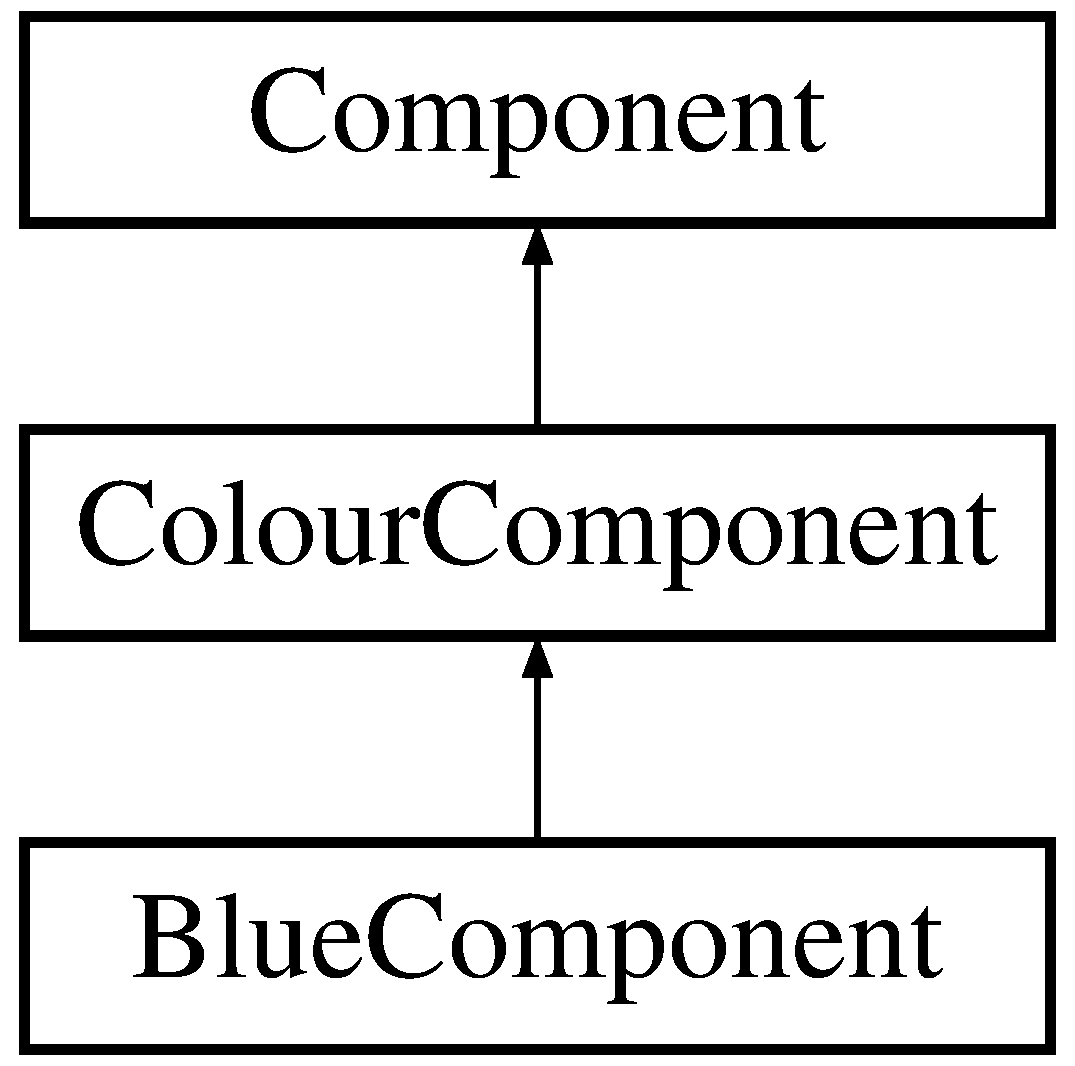
\includegraphics[height=3.000000cm]{class_blue_component}
\end{center}
\end{figure}
\subsection*{Additional Inherited Members}


The documentation for this class was generated from the following file\+:\begin{DoxyCompactItemize}
\item 
Game\+Engine/include/\mbox{\hyperlink{_colour_component_8h}{Colour\+Component.\+h}}\end{DoxyCompactItemize}

\hypertarget{class_camera}{}\section{Camera Class Reference}
\label{class_camera}\index{Camera@{Camera}}


{\ttfamily \#include $<$Camera.\+h$>$}

\subsection*{Public Member Functions}
\begin{DoxyCompactItemize}
\item 
\mbox{\hyperlink{class_camera_a01f94c3543f56ede7af49dc778f19331}{Camera}} ()
\item 
\mbox{\hyperlink{class_camera_acee2a1b3d56b0f141a3c6ee82735ed39}{Camera}} (const glm\+::vec3 \&pos)
\item 
\mbox{\hyperlink{class_camera_a9e5dda23dca2ae363424f7a9025f55c9}{Camera}} (const glm\+::vec3 \&pos, const glm\+::quat \&orient)
\item 
void \mbox{\hyperlink{class_camera_aec0442093303b9568a159f8c87f8b7d8}{look\+At}} (const glm\+::vec3 \&target)
\item 
const glm\+::vec3 \& \mbox{\hyperlink{class_camera_a26f5c28317ec7add2a21ddbdc8e463fb}{position}} () const
\item 
const glm\+::quat \& \mbox{\hyperlink{class_camera_a872dd113215278493380d19716c63644}{orientation}} () const
\item 
glm\+::mat4 \mbox{\hyperlink{class_camera_a2f90e661a78172675ca06ea69667b531}{get\+View\+Matrix}} () const
\item 
void \mbox{\hyperlink{class_camera_aa00429d00bae4984467f9c5d1a3bd158}{translate}} (const glm\+::vec3 \&v)
\item 
void \mbox{\hyperlink{class_camera_ac9e53556c53beee69c77a97e2a1c1068}{translate}} (float x, float y, float z)
\item 
void \mbox{\hyperlink{class_camera_a0e6180b5a8da63a999db3de1802c8f4c}{rotate}} (float angle, const glm\+::vec3 \&axis)
\item 
void \mbox{\hyperlink{class_camera_a4a45040f06f24a53af7f17bbcc610f22}{rotate}} (float angle, float x, float y, float z)
\item 
void \mbox{\hyperlink{class_camera_ab4eab94754431725c572d528a07a35cc}{yaw}} (float angle)
\item 
void \mbox{\hyperlink{class_camera_a49e00b90b94853e4485a6bdf063796de}{pitch}} (float angle)
\item 
void \mbox{\hyperlink{class_camera_a72be99f88b1cc21122178109d3441818}{roll}} (float angle)
\item 
void \mbox{\hyperlink{class_camera_ade53ee61895c2143da3cec03d08ef3eb}{set\+F\+OV}} (float fov)
\item 
const float \mbox{\hyperlink{class_camera_ab16a5e8f683ee2d598578a2d9836a24a}{get\+F\+OV}} () const
\end{DoxyCompactItemize}
\subsection*{Public Attributes}
\begin{DoxyCompactItemize}
\item 
glm\+::vec3 \mbox{\hyperlink{class_camera_aa4d06d49524248f81823444fa2544da0}{m\+\_\+position}}
\item 
glm\+::quat \mbox{\hyperlink{class_camera_ac035d6cb4b4bae255d6d12f51137357e}{m\+\_\+orientation}}
\item 
float \mbox{\hyperlink{class_camera_aa404a4e057fa16fb82ce8668d7a661b6}{m\+\_\+fov}}
\end{DoxyCompactItemize}


\subsection{Detailed Description}
class \mbox{\hyperlink{class_the}{The}} camera will be used to display all of the items in the scene. 

\subsection{Constructor \& Destructor Documentation}
\mbox{\Hypertarget{class_camera_a01f94c3543f56ede7af49dc778f19331}\label{class_camera_a01f94c3543f56ede7af49dc778f19331}} 
\index{Camera@{Camera}!Camera@{Camera}}
\index{Camera@{Camera}!Camera@{Camera}}
\subsubsection{\texorpdfstring{Camera()}{Camera()}\hspace{0.1cm}{\footnotesize\ttfamily [1/3]}}
{\footnotesize\ttfamily Camera\+::\+Camera (\begin{DoxyParamCaption}{ }\end{DoxyParamCaption})\hspace{0.3cm}{\ttfamily [inline]}}

Constructor \mbox{\Hypertarget{class_camera_acee2a1b3d56b0f141a3c6ee82735ed39}\label{class_camera_acee2a1b3d56b0f141a3c6ee82735ed39}} 
\index{Camera@{Camera}!Camera@{Camera}}
\index{Camera@{Camera}!Camera@{Camera}}
\subsubsection{\texorpdfstring{Camera()}{Camera()}\hspace{0.1cm}{\footnotesize\ttfamily [2/3]}}
{\footnotesize\ttfamily Camera\+::\+Camera (\begin{DoxyParamCaption}\item[{const glm\+::vec3 \&}]{pos }\end{DoxyParamCaption})\hspace{0.3cm}{\ttfamily [inline]}}

Constructor Param One \+: \mbox{\hyperlink{class_the}{The}} starting position for the camera. \mbox{\Hypertarget{class_camera_a9e5dda23dca2ae363424f7a9025f55c9}\label{class_camera_a9e5dda23dca2ae363424f7a9025f55c9}} 
\index{Camera@{Camera}!Camera@{Camera}}
\index{Camera@{Camera}!Camera@{Camera}}
\subsubsection{\texorpdfstring{Camera()}{Camera()}\hspace{0.1cm}{\footnotesize\ttfamily [3/3]}}
{\footnotesize\ttfamily Camera\+::\+Camera (\begin{DoxyParamCaption}\item[{const glm\+::vec3 \&}]{pos,  }\item[{const glm\+::quat \&}]{orient }\end{DoxyParamCaption})\hspace{0.3cm}{\ttfamily [inline]}}

Constructor Param One \+: \mbox{\hyperlink{class_the}{The}} starting position for the camera. Param Two \+: \mbox{\hyperlink{class_the}{The}} orientation for the starting camera. 

\subsection{Member Function Documentation}
\mbox{\Hypertarget{class_camera_ab16a5e8f683ee2d598578a2d9836a24a}\label{class_camera_ab16a5e8f683ee2d598578a2d9836a24a}} 
\index{Camera@{Camera}!get\+F\+OV@{get\+F\+OV}}
\index{get\+F\+OV@{get\+F\+OV}!Camera@{Camera}}
\subsubsection{\texorpdfstring{get\+F\+O\+V()}{getFOV()}}
{\footnotesize\ttfamily const float Camera\+::get\+F\+OV (\begin{DoxyParamCaption}{ }\end{DoxyParamCaption}) const\hspace{0.3cm}{\ttfamily [inline]}}

Get\+F\+OV \+: \mbox{\hyperlink{class_this}{This}} will be used to get the current field of view. \mbox{\Hypertarget{class_camera_a2f90e661a78172675ca06ea69667b531}\label{class_camera_a2f90e661a78172675ca06ea69667b531}} 
\index{Camera@{Camera}!get\+View\+Matrix@{get\+View\+Matrix}}
\index{get\+View\+Matrix@{get\+View\+Matrix}!Camera@{Camera}}
\subsubsection{\texorpdfstring{get\+View\+Matrix()}{getViewMatrix()}}
{\footnotesize\ttfamily glm\+::mat4 Camera\+::get\+View\+Matrix (\begin{DoxyParamCaption}{ }\end{DoxyParamCaption}) const\hspace{0.3cm}{\ttfamily [inline]}}

Get\+View\+Matrix \+: \mbox{\hyperlink{class_this}{This}} will be used to transform vertices from world space to view space. \mbox{\Hypertarget{class_camera_aec0442093303b9568a159f8c87f8b7d8}\label{class_camera_aec0442093303b9568a159f8c87f8b7d8}} 
\index{Camera@{Camera}!look\+At@{look\+At}}
\index{look\+At@{look\+At}!Camera@{Camera}}
\subsubsection{\texorpdfstring{look\+At()}{lookAt()}}
{\footnotesize\ttfamily void Camera\+::look\+At (\begin{DoxyParamCaption}\item[{const glm\+::vec3 \&}]{target }\end{DoxyParamCaption})\hspace{0.3cm}{\ttfamily [inline]}}

Look\+At \+: \mbox{\hyperlink{class_this}{This}} will be used to point the camera at a specific target. Param One \+: \mbox{\hyperlink{class_the}{The}} vector3 for the target you wish to look at. \mbox{\Hypertarget{class_camera_a872dd113215278493380d19716c63644}\label{class_camera_a872dd113215278493380d19716c63644}} 
\index{Camera@{Camera}!orientation@{orientation}}
\index{orientation@{orientation}!Camera@{Camera}}
\subsubsection{\texorpdfstring{orientation()}{orientation()}}
{\footnotesize\ttfamily const glm\+::quat\& Camera\+::orientation (\begin{DoxyParamCaption}{ }\end{DoxyParamCaption}) const\hspace{0.3cm}{\ttfamily [inline]}}

Orientation \+: \mbox{\hyperlink{class_this}{This}} will return the current orientation of the camera. \mbox{\Hypertarget{class_camera_a49e00b90b94853e4485a6bdf063796de}\label{class_camera_a49e00b90b94853e4485a6bdf063796de}} 
\index{Camera@{Camera}!pitch@{pitch}}
\index{pitch@{pitch}!Camera@{Camera}}
\subsubsection{\texorpdfstring{pitch()}{pitch()}}
{\footnotesize\ttfamily void Camera\+::pitch (\begin{DoxyParamCaption}\item[{float}]{angle }\end{DoxyParamCaption})\hspace{0.3cm}{\ttfamily [inline]}}

Pitch \+: \mbox{\hyperlink{class_this}{This}} will rotate the camera by the angle around the Y-\/\+Axis. Param One \+: \mbox{\hyperlink{class_the}{The}} angle of which to rotate by. \mbox{\Hypertarget{class_camera_a26f5c28317ec7add2a21ddbdc8e463fb}\label{class_camera_a26f5c28317ec7add2a21ddbdc8e463fb}} 
\index{Camera@{Camera}!position@{position}}
\index{position@{position}!Camera@{Camera}}
\subsubsection{\texorpdfstring{position()}{position()}}
{\footnotesize\ttfamily const glm\+::vec3\& Camera\+::position (\begin{DoxyParamCaption}{ }\end{DoxyParamCaption}) const\hspace{0.3cm}{\ttfamily [inline]}}

Position \+: \mbox{\hyperlink{class_this}{This}} will return the current position of the camera. \mbox{\Hypertarget{class_camera_a72be99f88b1cc21122178109d3441818}\label{class_camera_a72be99f88b1cc21122178109d3441818}} 
\index{Camera@{Camera}!roll@{roll}}
\index{roll@{roll}!Camera@{Camera}}
\subsubsection{\texorpdfstring{roll()}{roll()}}
{\footnotesize\ttfamily void Camera\+::roll (\begin{DoxyParamCaption}\item[{float}]{angle }\end{DoxyParamCaption})\hspace{0.3cm}{\ttfamily [inline]}}

Roll \+: \mbox{\hyperlink{class_this}{This}} will rotate the camera by the angle around the X-\/\+Axis. Param One \+: \mbox{\hyperlink{class_the}{The}} angle of which to rotate by. \mbox{\Hypertarget{class_camera_a0e6180b5a8da63a999db3de1802c8f4c}\label{class_camera_a0e6180b5a8da63a999db3de1802c8f4c}} 
\index{Camera@{Camera}!rotate@{rotate}}
\index{rotate@{rotate}!Camera@{Camera}}
\subsubsection{\texorpdfstring{rotate()}{rotate()}\hspace{0.1cm}{\footnotesize\ttfamily [1/2]}}
{\footnotesize\ttfamily void Camera\+::rotate (\begin{DoxyParamCaption}\item[{float}]{angle,  }\item[{const glm\+::vec3 \&}]{axis }\end{DoxyParamCaption})\hspace{0.3cm}{\ttfamily [inline]}}

Rotate \+: \mbox{\hyperlink{class_this}{This}} will rotate the camera by a specific angle. ~\newline
Param One \+: \mbox{\hyperlink{class_the}{The}} angle in which to rotate by. Param Two \+: \mbox{\hyperlink{class_the}{The}} axis to rotate the camrea around. \mbox{\Hypertarget{class_camera_a4a45040f06f24a53af7f17bbcc610f22}\label{class_camera_a4a45040f06f24a53af7f17bbcc610f22}} 
\index{Camera@{Camera}!rotate@{rotate}}
\index{rotate@{rotate}!Camera@{Camera}}
\subsubsection{\texorpdfstring{rotate()}{rotate()}\hspace{0.1cm}{\footnotesize\ttfamily [2/2]}}
{\footnotesize\ttfamily void Camera\+::rotate (\begin{DoxyParamCaption}\item[{float}]{angle,  }\item[{float}]{x,  }\item[{float}]{y,  }\item[{float}]{z }\end{DoxyParamCaption})\hspace{0.3cm}{\ttfamily [inline]}}

Rotate \+: \mbox{\hyperlink{class_this}{This}} will rotate the camera by a specific angle. Param One \+: \mbox{\hyperlink{class_the}{The}} angle in which to rotate by. Param Two \+: \mbox{\hyperlink{class_the}{The}} new X value for the rotation\textquotesingle{}s axis. Param Three \+: \mbox{\hyperlink{class_the}{The}} new Y value for the rotation\textquotesingle{}s axis. Param Four \+: \mbox{\hyperlink{class_the}{The}} new Z value for the rotation\textquotesingle{}s axis. \mbox{\Hypertarget{class_camera_ade53ee61895c2143da3cec03d08ef3eb}\label{class_camera_ade53ee61895c2143da3cec03d08ef3eb}} 
\index{Camera@{Camera}!set\+F\+OV@{set\+F\+OV}}
\index{set\+F\+OV@{set\+F\+OV}!Camera@{Camera}}
\subsubsection{\texorpdfstring{set\+F\+O\+V()}{setFOV()}}
{\footnotesize\ttfamily void Camera\+::set\+F\+OV (\begin{DoxyParamCaption}\item[{float}]{fov }\end{DoxyParamCaption})\hspace{0.3cm}{\ttfamily [inline]}}

Set\+F\+OV \+: \mbox{\hyperlink{class_this}{This}} will set a new value for the camera\textquotesingle{}s field of view. Param One \+: \mbox{\hyperlink{class_the}{The}} new field of view for the camera. \mbox{\Hypertarget{class_camera_aa00429d00bae4984467f9c5d1a3bd158}\label{class_camera_aa00429d00bae4984467f9c5d1a3bd158}} 
\index{Camera@{Camera}!translate@{translate}}
\index{translate@{translate}!Camera@{Camera}}
\subsubsection{\texorpdfstring{translate()}{translate()}\hspace{0.1cm}{\footnotesize\ttfamily [1/2]}}
{\footnotesize\ttfamily void Camera\+::translate (\begin{DoxyParamCaption}\item[{const glm\+::vec3 \&}]{v }\end{DoxyParamCaption})\hspace{0.3cm}{\ttfamily [inline]}}

Translate \+: \mbox{\hyperlink{class_this}{This}} will move the camera in the game space. Param One \+: A combination of X, Y and Z values for the new position. \mbox{\Hypertarget{class_camera_ac9e53556c53beee69c77a97e2a1c1068}\label{class_camera_ac9e53556c53beee69c77a97e2a1c1068}} 
\index{Camera@{Camera}!translate@{translate}}
\index{translate@{translate}!Camera@{Camera}}
\subsubsection{\texorpdfstring{translate()}{translate()}\hspace{0.1cm}{\footnotesize\ttfamily [2/2]}}
{\footnotesize\ttfamily void Camera\+::translate (\begin{DoxyParamCaption}\item[{float}]{x,  }\item[{float}]{y,  }\item[{float}]{z }\end{DoxyParamCaption})\hspace{0.3cm}{\ttfamily [inline]}}

Translate \+: \mbox{\hyperlink{class_this}{This}} will move the camera in the game space. Param One \+: \mbox{\hyperlink{class_the}{The}} new X value for the camera. Param Two \+: \mbox{\hyperlink{class_the}{The}} new Y value for the camera. Param Three \+: \mbox{\hyperlink{class_the}{The}} new Z value for the camera. \mbox{\Hypertarget{class_camera_ab4eab94754431725c572d528a07a35cc}\label{class_camera_ab4eab94754431725c572d528a07a35cc}} 
\index{Camera@{Camera}!yaw@{yaw}}
\index{yaw@{yaw}!Camera@{Camera}}
\subsubsection{\texorpdfstring{yaw()}{yaw()}}
{\footnotesize\ttfamily void Camera\+::yaw (\begin{DoxyParamCaption}\item[{float}]{angle }\end{DoxyParamCaption})\hspace{0.3cm}{\ttfamily [inline]}}

Yaw \+: \mbox{\hyperlink{class_this}{This}} will rotate the camera by the angle around the Z-\/\+Axis. Param One \+: \mbox{\hyperlink{class_the}{The}} angle of which to rotate by. 

\subsection{Member Data Documentation}
\mbox{\Hypertarget{class_camera_aa404a4e057fa16fb82ce8668d7a661b6}\label{class_camera_aa404a4e057fa16fb82ce8668d7a661b6}} 
\index{Camera@{Camera}!m\+\_\+fov@{m\+\_\+fov}}
\index{m\+\_\+fov@{m\+\_\+fov}!Camera@{Camera}}
\subsubsection{\texorpdfstring{m\+\_\+fov}{m\_fov}}
{\footnotesize\ttfamily float Camera\+::m\+\_\+fov}

\mbox{\Hypertarget{class_camera_ac035d6cb4b4bae255d6d12f51137357e}\label{class_camera_ac035d6cb4b4bae255d6d12f51137357e}} 
\index{Camera@{Camera}!m\+\_\+orientation@{m\+\_\+orientation}}
\index{m\+\_\+orientation@{m\+\_\+orientation}!Camera@{Camera}}
\subsubsection{\texorpdfstring{m\+\_\+orientation}{m\_orientation}}
{\footnotesize\ttfamily glm\+::quat Camera\+::m\+\_\+orientation}

\mbox{\Hypertarget{class_camera_aa4d06d49524248f81823444fa2544da0}\label{class_camera_aa4d06d49524248f81823444fa2544da0}} 
\index{Camera@{Camera}!m\+\_\+position@{m\+\_\+position}}
\index{m\+\_\+position@{m\+\_\+position}!Camera@{Camera}}
\subsubsection{\texorpdfstring{m\+\_\+position}{m\_position}}
{\footnotesize\ttfamily glm\+::vec3 Camera\+::m\+\_\+position}



The documentation for this class was generated from the following file\+:\begin{DoxyCompactItemize}
\item 
Game\+Engine/include/\mbox{\hyperlink{_camera_8h}{Camera.\+h}}\end{DoxyCompactItemize}

\hypertarget{class_camera_component}{}\section{Camera\+Component Class Reference}
\label{class_camera_component}\index{Camera\+Component@{Camera\+Component}}


{\ttfamily \#include $<$Camera\+Component.\+h$>$}

Inheritance diagram for Camera\+Component\+:\begin{figure}[H]
\begin{center}
\leavevmode
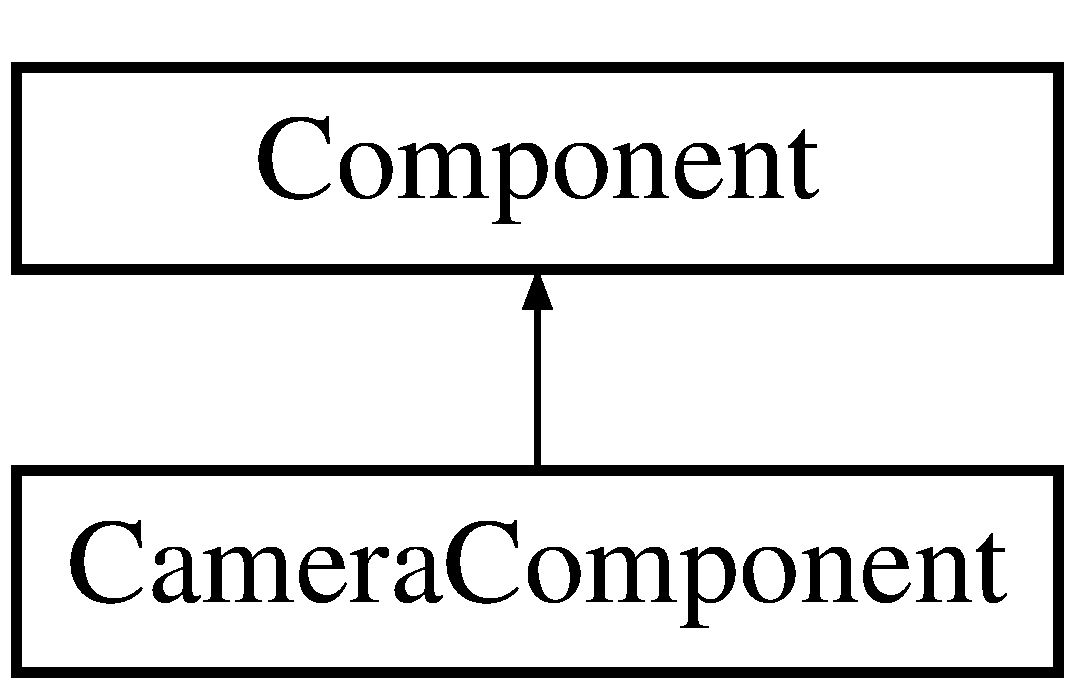
\includegraphics[height=2.000000cm]{class_camera_component}
\end{center}
\end{figure}
\subsection*{Public Member Functions}
\begin{DoxyCompactItemize}
\item 
\mbox{\hyperlink{class_camera_component_a54997069f98c746e4d6df9e2ce8b5416}{Camera\+Component}} (\mbox{\hyperlink{class_camera}{Camera}} $\ast$connect\+Camera, \mbox{\hyperlink{class_game_object}{Game\+Object}} $\ast$connect\+Object)
\item 
\mbox{\hyperlink{class_camera_component_a638e0e8bf55a52b735f8ab08eb0ad631}{Camera\+Component}} (\mbox{\hyperlink{class_camera}{Camera}} $\ast$connect\+Camera, \mbox{\hyperlink{class_game_object}{Game\+Object}} $\ast$connect\+Object, glm\+::vec3 offset)
\item 
\mbox{\hyperlink{class_camera_component_a05759ae68f3830c8b79314640ad1471c}{Camera\+Component}} (\mbox{\hyperlink{class_camera}{Camera}} $\ast$connect\+Camera, \mbox{\hyperlink{class_game_object}{Game\+Object}} $\ast$connect\+Object, \mbox{\hyperlink{_camera_component_8h_ab07ecb557631c59d8b7ec9c3db110dd5}{camera\+Type}} selection)
\item 
\mbox{\hyperlink{class_camera_component_aab0e46dcfc4a845c7373fe1142d4c981}{Camera\+Component}} (\mbox{\hyperlink{class_camera}{Camera}} $\ast$connect\+Camera, \mbox{\hyperlink{class_game_object}{Game\+Object}} $\ast$connect\+Object, glm\+::vec3 offset, \mbox{\hyperlink{_camera_component_8h_ab07ecb557631c59d8b7ec9c3db110dd5}{camera\+Type}} selection)
\item 
\mbox{\hyperlink{class_camera_component_a977e080c45152719c5e6335cfb0698fc}{$\sim$\+Camera\+Component}} ()
\item 
\mbox{\hyperlink{class_camera}{Camera}} \& \mbox{\hyperlink{class_camera_component_a1fbb5ea1f011ec8ea75688566c8bb545}{m\+\_\+\+Get\+Camera}} ()
\item 
void \mbox{\hyperlink{class_camera_component_a4db1be92619451a81d54269e13232a1f}{m\+\_\+\+Set\+Camera\+Offset}} (glm\+::vec3 new\+Camera\+Offset)
\item 
void \mbox{\hyperlink{class_camera_component_aee0c00e1dbb83fd953b718e278c90603}{m\+\_\+\+Set\+Camera\+Type}} (\mbox{\hyperlink{_camera_component_8h_ab07ecb557631c59d8b7ec9c3db110dd5}{camera\+Type}} new\+Type)
\item 
void \mbox{\hyperlink{class_camera_component_aa0391037fd478ea1a602835ea64091ba}{On\+Update}} (float dt) override
\item 
void \mbox{\hyperlink{class_camera_component_a1cd7e6036568be5bf45d249d8f96a596}{On\+Message}} (const std\+::string m) override
\end{DoxyCompactItemize}
\subsection*{Public Attributes}
\begin{DoxyCompactItemize}
\item 
\mbox{\hyperlink{_camera_component_8h_ab07ecb557631c59d8b7ec9c3db110dd5}{camera\+Type}} \mbox{\hyperlink{class_camera_component_ac2c53e574361e9069c32baa344e90eae}{m\+\_\+\+Camera\+Type}}
\end{DoxyCompactItemize}


\subsection{Constructor \& Destructor Documentation}
\mbox{\Hypertarget{class_camera_component_a54997069f98c746e4d6df9e2ce8b5416}\label{class_camera_component_a54997069f98c746e4d6df9e2ce8b5416}} 
\index{Camera\+Component@{Camera\+Component}!Camera\+Component@{Camera\+Component}}
\index{Camera\+Component@{Camera\+Component}!Camera\+Component@{Camera\+Component}}
\subsubsection{\texorpdfstring{Camera\+Component()}{CameraComponent()}\hspace{0.1cm}{\footnotesize\ttfamily [1/4]}}
{\footnotesize\ttfamily Camera\+Component\+::\+Camera\+Component (\begin{DoxyParamCaption}\item[{\mbox{\hyperlink{class_camera}{Camera}} $\ast$}]{connect\+Camera,  }\item[{\mbox{\hyperlink{class_game_object}{Game\+Object}} $\ast$}]{connect\+Object }\end{DoxyParamCaption})\hspace{0.3cm}{\ttfamily [inline]}}

Constructor Param One \+: \mbox{\hyperlink{class_the}{The}} camera object connected to this object. Param Two \+: \mbox{\hyperlink{class_the}{The}} game object this component is connected to. \mbox{\Hypertarget{class_camera_component_a638e0e8bf55a52b735f8ab08eb0ad631}\label{class_camera_component_a638e0e8bf55a52b735f8ab08eb0ad631}} 
\index{Camera\+Component@{Camera\+Component}!Camera\+Component@{Camera\+Component}}
\index{Camera\+Component@{Camera\+Component}!Camera\+Component@{Camera\+Component}}
\subsubsection{\texorpdfstring{Camera\+Component()}{CameraComponent()}\hspace{0.1cm}{\footnotesize\ttfamily [2/4]}}
{\footnotesize\ttfamily Camera\+Component\+::\+Camera\+Component (\begin{DoxyParamCaption}\item[{\mbox{\hyperlink{class_camera}{Camera}} $\ast$}]{connect\+Camera,  }\item[{\mbox{\hyperlink{class_game_object}{Game\+Object}} $\ast$}]{connect\+Object,  }\item[{glm\+::vec3}]{offset }\end{DoxyParamCaption})\hspace{0.3cm}{\ttfamily [inline]}}

Constructor Param One \+: \mbox{\hyperlink{class_the}{The}} camera object connected to this object. Param Two \+: \mbox{\hyperlink{class_the}{The}} game object this component is connected to. Param Three \+: \mbox{\hyperlink{class_the}{The}} offset of the camera from the game object. \mbox{\Hypertarget{class_camera_component_a05759ae68f3830c8b79314640ad1471c}\label{class_camera_component_a05759ae68f3830c8b79314640ad1471c}} 
\index{Camera\+Component@{Camera\+Component}!Camera\+Component@{Camera\+Component}}
\index{Camera\+Component@{Camera\+Component}!Camera\+Component@{Camera\+Component}}
\subsubsection{\texorpdfstring{Camera\+Component()}{CameraComponent()}\hspace{0.1cm}{\footnotesize\ttfamily [3/4]}}
{\footnotesize\ttfamily Camera\+Component\+::\+Camera\+Component (\begin{DoxyParamCaption}\item[{\mbox{\hyperlink{class_camera}{Camera}} $\ast$}]{connect\+Camera,  }\item[{\mbox{\hyperlink{class_game_object}{Game\+Object}} $\ast$}]{connect\+Object,  }\item[{\mbox{\hyperlink{_camera_component_8h_ab07ecb557631c59d8b7ec9c3db110dd5}{camera\+Type}}}]{selection }\end{DoxyParamCaption})\hspace{0.3cm}{\ttfamily [inline]}}

Constructor Param One \+: \mbox{\hyperlink{class_the}{The}} camera object connected to this object. Param Two \+: \mbox{\hyperlink{class_the}{The}} game object this component is connected to. Param Three \+: \mbox{\hyperlink{class_the}{The}} type for this camera. \mbox{\Hypertarget{class_camera_component_aab0e46dcfc4a845c7373fe1142d4c981}\label{class_camera_component_aab0e46dcfc4a845c7373fe1142d4c981}} 
\index{Camera\+Component@{Camera\+Component}!Camera\+Component@{Camera\+Component}}
\index{Camera\+Component@{Camera\+Component}!Camera\+Component@{Camera\+Component}}
\subsubsection{\texorpdfstring{Camera\+Component()}{CameraComponent()}\hspace{0.1cm}{\footnotesize\ttfamily [4/4]}}
{\footnotesize\ttfamily Camera\+Component\+::\+Camera\+Component (\begin{DoxyParamCaption}\item[{\mbox{\hyperlink{class_camera}{Camera}} $\ast$}]{connect\+Camera,  }\item[{\mbox{\hyperlink{class_game_object}{Game\+Object}} $\ast$}]{connect\+Object,  }\item[{glm\+::vec3}]{offset,  }\item[{\mbox{\hyperlink{_camera_component_8h_ab07ecb557631c59d8b7ec9c3db110dd5}{camera\+Type}}}]{selection }\end{DoxyParamCaption})\hspace{0.3cm}{\ttfamily [inline]}}

Constructor Param One \+: \mbox{\hyperlink{class_the}{The}} camera object connected to this object. Param Two \+: \mbox{\hyperlink{class_the}{The}} game object this component is connected to. Param Three \+: \mbox{\hyperlink{class_the}{The}} offset of the camera from the game object. Param Four \+: \mbox{\hyperlink{class_the}{The}} type for this camera. \mbox{\Hypertarget{class_camera_component_a977e080c45152719c5e6335cfb0698fc}\label{class_camera_component_a977e080c45152719c5e6335cfb0698fc}} 
\index{Camera\+Component@{Camera\+Component}!````~Camera\+Component@{$\sim$\+Camera\+Component}}
\index{````~Camera\+Component@{$\sim$\+Camera\+Component}!Camera\+Component@{Camera\+Component}}
\subsubsection{\texorpdfstring{$\sim$\+Camera\+Component()}{~CameraComponent()}}
{\footnotesize\ttfamily Camera\+Component\+::$\sim$\+Camera\+Component (\begin{DoxyParamCaption}{ }\end{DoxyParamCaption})\hspace{0.3cm}{\ttfamily [inline]}}

Deconstructor 

\subsection{Member Function Documentation}
\mbox{\Hypertarget{class_camera_component_a1fbb5ea1f011ec8ea75688566c8bb545}\label{class_camera_component_a1fbb5ea1f011ec8ea75688566c8bb545}} 
\index{Camera\+Component@{Camera\+Component}!m\+\_\+\+Get\+Camera@{m\+\_\+\+Get\+Camera}}
\index{m\+\_\+\+Get\+Camera@{m\+\_\+\+Get\+Camera}!Camera\+Component@{Camera\+Component}}
\subsubsection{\texorpdfstring{m\+\_\+\+Get\+Camera()}{m\_GetCamera()}}
{\footnotesize\ttfamily \mbox{\hyperlink{class_camera}{Camera}}\& Camera\+Component\+::m\+\_\+\+Get\+Camera (\begin{DoxyParamCaption}{ }\end{DoxyParamCaption})\hspace{0.3cm}{\ttfamily [inline]}}

Get\+Camera \+: \mbox{\hyperlink{class_this}{This}} will return the connected game object. \mbox{\Hypertarget{class_camera_component_a4db1be92619451a81d54269e13232a1f}\label{class_camera_component_a4db1be92619451a81d54269e13232a1f}} 
\index{Camera\+Component@{Camera\+Component}!m\+\_\+\+Set\+Camera\+Offset@{m\+\_\+\+Set\+Camera\+Offset}}
\index{m\+\_\+\+Set\+Camera\+Offset@{m\+\_\+\+Set\+Camera\+Offset}!Camera\+Component@{Camera\+Component}}
\subsubsection{\texorpdfstring{m\+\_\+\+Set\+Camera\+Offset()}{m\_SetCameraOffset()}}
{\footnotesize\ttfamily void Camera\+Component\+::m\+\_\+\+Set\+Camera\+Offset (\begin{DoxyParamCaption}\item[{glm\+::vec3}]{new\+Camera\+Offset }\end{DoxyParamCaption})\hspace{0.3cm}{\ttfamily [inline]}}

Set\+Camera\+Offset Param One \+: \mbox{\hyperlink{class_the}{The}} vector (X, Y, Z) to offset the camera by. \mbox{\Hypertarget{class_camera_component_aee0c00e1dbb83fd953b718e278c90603}\label{class_camera_component_aee0c00e1dbb83fd953b718e278c90603}} 
\index{Camera\+Component@{Camera\+Component}!m\+\_\+\+Set\+Camera\+Type@{m\+\_\+\+Set\+Camera\+Type}}
\index{m\+\_\+\+Set\+Camera\+Type@{m\+\_\+\+Set\+Camera\+Type}!Camera\+Component@{Camera\+Component}}
\subsubsection{\texorpdfstring{m\+\_\+\+Set\+Camera\+Type()}{m\_SetCameraType()}}
{\footnotesize\ttfamily void Camera\+Component\+::m\+\_\+\+Set\+Camera\+Type (\begin{DoxyParamCaption}\item[{\mbox{\hyperlink{_camera_component_8h_ab07ecb557631c59d8b7ec9c3db110dd5}{camera\+Type}}}]{new\+Type }\end{DoxyParamCaption})\hspace{0.3cm}{\ttfamily [inline]}}

Set\+Camera\+Type \+: \mbox{\hyperlink{class_this}{This}} will be used to set the type for the camera. Param One \+: \mbox{\hyperlink{class_the}{The}} new type for the camera. \mbox{\Hypertarget{class_camera_component_a1cd7e6036568be5bf45d249d8f96a596}\label{class_camera_component_a1cd7e6036568be5bf45d249d8f96a596}} 
\index{Camera\+Component@{Camera\+Component}!On\+Message@{On\+Message}}
\index{On\+Message@{On\+Message}!Camera\+Component@{Camera\+Component}}
\subsubsection{\texorpdfstring{On\+Message()}{OnMessage()}}
{\footnotesize\ttfamily void Camera\+Component\+::\+On\+Message (\begin{DoxyParamCaption}\item[{const std\+::string}]{m }\end{DoxyParamCaption})\hspace{0.3cm}{\ttfamily [inline]}, {\ttfamily [override]}, {\ttfamily [virtual]}}

On\+Message \+: \mbox{\hyperlink{class_this}{This}} will be use to react to a key press if required. 

Implements \mbox{\hyperlink{class_component_a1a880fe5e212cd7ef8241e220660417d}{Component}}.

\mbox{\Hypertarget{class_camera_component_aa0391037fd478ea1a602835ea64091ba}\label{class_camera_component_aa0391037fd478ea1a602835ea64091ba}} 
\index{Camera\+Component@{Camera\+Component}!On\+Update@{On\+Update}}
\index{On\+Update@{On\+Update}!Camera\+Component@{Camera\+Component}}
\subsubsection{\texorpdfstring{On\+Update()}{OnUpdate()}}
{\footnotesize\ttfamily void Camera\+Component\+::\+On\+Update (\begin{DoxyParamCaption}\item[{float}]{dt }\end{DoxyParamCaption})\hspace{0.3cm}{\ttfamily [inline]}, {\ttfamily [override]}, {\ttfamily [virtual]}}

On\+Update \+: \mbox{\hyperlink{class_this}{This}} will be used to call any update functions for this component. 

Implements \mbox{\hyperlink{class_component_ab71d7f4b6d8792287a9b0c9e045acbe0}{Component}}.



\subsection{Member Data Documentation}
\mbox{\Hypertarget{class_camera_component_ac2c53e574361e9069c32baa344e90eae}\label{class_camera_component_ac2c53e574361e9069c32baa344e90eae}} 
\index{Camera\+Component@{Camera\+Component}!m\+\_\+\+Camera\+Type@{m\+\_\+\+Camera\+Type}}
\index{m\+\_\+\+Camera\+Type@{m\+\_\+\+Camera\+Type}!Camera\+Component@{Camera\+Component}}
\subsubsection{\texorpdfstring{m\+\_\+\+Camera\+Type}{m\_CameraType}}
{\footnotesize\ttfamily \mbox{\hyperlink{_camera_component_8h_ab07ecb557631c59d8b7ec9c3db110dd5}{camera\+Type}} Camera\+Component\+::m\+\_\+\+Camera\+Type}



The documentation for this class was generated from the following file\+:\begin{DoxyCompactItemize}
\item 
Game\+Engine/include/\mbox{\hyperlink{_camera_component_8h}{Camera\+Component.\+h}}\end{DoxyCompactItemize}

\hypertarget{class_colour_component}{}\section{Colour\+Component Class Reference}
\label{class_colour_component}\index{Colour\+Component@{Colour\+Component}}


{\ttfamily \#include $<$Colour\+Component.\+h$>$}

Inheritance diagram for Colour\+Component\+:\begin{figure}[H]
\begin{center}
\leavevmode
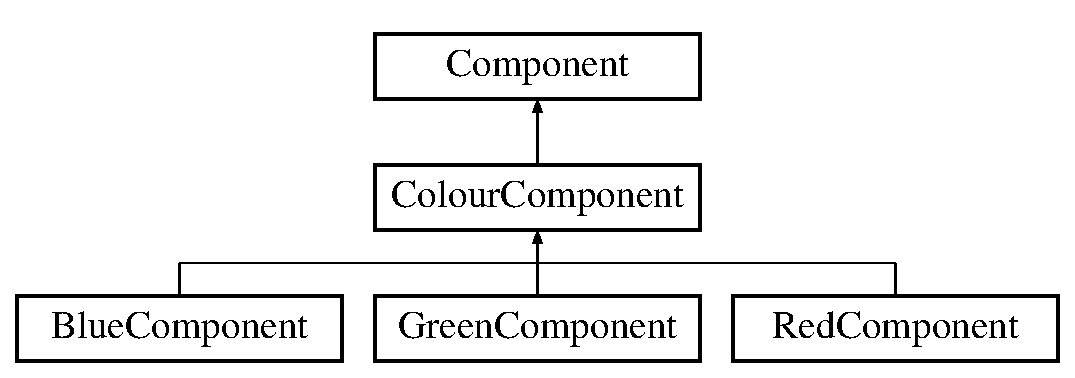
\includegraphics[height=3.000000cm]{class_colour_component}
\end{center}
\end{figure}
\subsection*{Public Member Functions}
\begin{DoxyCompactItemize}
\item 
\mbox{\hyperlink{class_colour_component_aea6cf99fa40f6ed6d670e89fab944b1c}{Colour\+Component}} ()
\item 
void \mbox{\hyperlink{class_colour_component_ae45e91aebb680031bb1328c7c189ea15}{On\+Update}} (float dt) override
\item 
void \mbox{\hyperlink{class_colour_component_a40b859f0c124ddbe92ff1e53bdb398a0}{On\+Message}} (const std\+::string m) override
\end{DoxyCompactItemize}
\subsection*{Public Attributes}
\begin{DoxyCompactItemize}
\item 
float \mbox{\hyperlink{class_colour_component_a58d3b68b7fdbf8acc74c043a05371216}{m\+\_\+colour\+Value}}
\end{DoxyCompactItemize}


\subsection{Constructor \& Destructor Documentation}
\mbox{\Hypertarget{class_colour_component_aea6cf99fa40f6ed6d670e89fab944b1c}\label{class_colour_component_aea6cf99fa40f6ed6d670e89fab944b1c}} 
\index{Colour\+Component@{Colour\+Component}!Colour\+Component@{Colour\+Component}}
\index{Colour\+Component@{Colour\+Component}!Colour\+Component@{Colour\+Component}}
\subsubsection{\texorpdfstring{Colour\+Component()}{ColourComponent()}}
{\footnotesize\ttfamily Colour\+Component\+::\+Colour\+Component (\begin{DoxyParamCaption}{ }\end{DoxyParamCaption})\hspace{0.3cm}{\ttfamily [inline]}}



\subsection{Member Function Documentation}
\mbox{\Hypertarget{class_colour_component_a40b859f0c124ddbe92ff1e53bdb398a0}\label{class_colour_component_a40b859f0c124ddbe92ff1e53bdb398a0}} 
\index{Colour\+Component@{Colour\+Component}!On\+Message@{On\+Message}}
\index{On\+Message@{On\+Message}!Colour\+Component@{Colour\+Component}}
\subsubsection{\texorpdfstring{On\+Message()}{OnMessage()}}
{\footnotesize\ttfamily void Colour\+Component\+::\+On\+Message (\begin{DoxyParamCaption}\item[{const std\+::string}]{m }\end{DoxyParamCaption})\hspace{0.3cm}{\ttfamily [inline]}, {\ttfamily [override]}, {\ttfamily [virtual]}}

On\+Message \+: \mbox{\hyperlink{class_this}{This}} will be use to react to a key press if required. 

Implements \mbox{\hyperlink{class_component_a1a880fe5e212cd7ef8241e220660417d}{Component}}.

\mbox{\Hypertarget{class_colour_component_ae45e91aebb680031bb1328c7c189ea15}\label{class_colour_component_ae45e91aebb680031bb1328c7c189ea15}} 
\index{Colour\+Component@{Colour\+Component}!On\+Update@{On\+Update}}
\index{On\+Update@{On\+Update}!Colour\+Component@{Colour\+Component}}
\subsubsection{\texorpdfstring{On\+Update()}{OnUpdate()}}
{\footnotesize\ttfamily void Colour\+Component\+::\+On\+Update (\begin{DoxyParamCaption}\item[{float}]{dt }\end{DoxyParamCaption})\hspace{0.3cm}{\ttfamily [inline]}, {\ttfamily [override]}, {\ttfamily [virtual]}}

On\+Update \+: \mbox{\hyperlink{class_this}{This}} will be used to call any update functions for this component. 

Implements \mbox{\hyperlink{class_component_ab71d7f4b6d8792287a9b0c9e045acbe0}{Component}}.



\subsection{Member Data Documentation}
\mbox{\Hypertarget{class_colour_component_a58d3b68b7fdbf8acc74c043a05371216}\label{class_colour_component_a58d3b68b7fdbf8acc74c043a05371216}} 
\index{Colour\+Component@{Colour\+Component}!m\+\_\+colour\+Value@{m\+\_\+colour\+Value}}
\index{m\+\_\+colour\+Value@{m\+\_\+colour\+Value}!Colour\+Component@{Colour\+Component}}
\subsubsection{\texorpdfstring{m\+\_\+colour\+Value}{m\_colourValue}}
{\footnotesize\ttfamily float Colour\+Component\+::m\+\_\+colour\+Value}



The documentation for this class was generated from the following file\+:\begin{DoxyCompactItemize}
\item 
Game\+Engine/include/\mbox{\hyperlink{_colour_component_8h}{Colour\+Component.\+h}}\end{DoxyCompactItemize}

\hypertarget{class_component}{}\section{Component Class Reference}
\label{class_component}\index{Component@{Component}}


{\ttfamily \#include $<$Component.\+h$>$}

Inheritance diagram for Component\+:\begin{figure}[H]
\begin{center}
\leavevmode
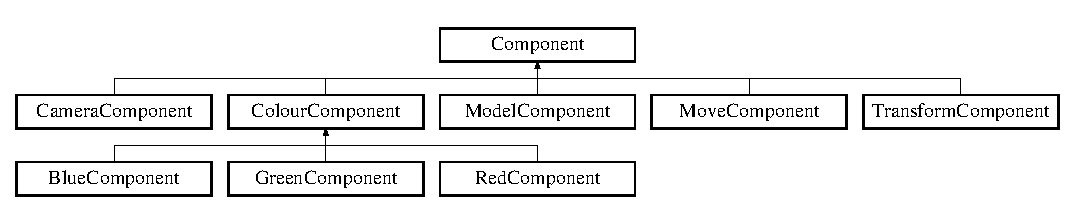
\includegraphics[height=2.400000cm]{class_component}
\end{center}
\end{figure}
\subsection*{Public Member Functions}
\begin{DoxyCompactItemize}
\item 
virtual void \mbox{\hyperlink{class_component_ab71d7f4b6d8792287a9b0c9e045acbe0}{On\+Update}} (float dt)=0
\item 
virtual void \mbox{\hyperlink{class_component_a1a880fe5e212cd7ef8241e220660417d}{On\+Message}} (const std\+::string m)=0
\end{DoxyCompactItemize}


\subsection{Member Function Documentation}
\mbox{\Hypertarget{class_component_a1a880fe5e212cd7ef8241e220660417d}\label{class_component_a1a880fe5e212cd7ef8241e220660417d}} 
\index{Component@{Component}!On\+Message@{On\+Message}}
\index{On\+Message@{On\+Message}!Component@{Component}}
\subsubsection{\texorpdfstring{On\+Message()}{OnMessage()}}
{\footnotesize\ttfamily virtual void Component\+::\+On\+Message (\begin{DoxyParamCaption}\item[{const std\+::string}]{m }\end{DoxyParamCaption})\hspace{0.3cm}{\ttfamily [pure virtual]}}

On\+Message \+: \mbox{\hyperlink{class_this}{This}} will be use to react to a key press if required. 

Implemented in \mbox{\hyperlink{class_camera_component_a1cd7e6036568be5bf45d249d8f96a596}{Camera\+Component}}, \mbox{\hyperlink{class_move_component_a27146b88beda6223ed9f4a82c47a917a}{Move\+Component}}, \mbox{\hyperlink{class_transform_component_ac250c4b7e47e639d0f8693d04c9b5051}{Transform\+Component}}, \mbox{\hyperlink{class_model_component_a48d6170e857f323839039ce54e9418e1}{Model\+Component}}, and \mbox{\hyperlink{class_colour_component_a40b859f0c124ddbe92ff1e53bdb398a0}{Colour\+Component}}.

\mbox{\Hypertarget{class_component_ab71d7f4b6d8792287a9b0c9e045acbe0}\label{class_component_ab71d7f4b6d8792287a9b0c9e045acbe0}} 
\index{Component@{Component}!On\+Update@{On\+Update}}
\index{On\+Update@{On\+Update}!Component@{Component}}
\subsubsection{\texorpdfstring{On\+Update()}{OnUpdate()}}
{\footnotesize\ttfamily virtual void Component\+::\+On\+Update (\begin{DoxyParamCaption}\item[{float}]{dt }\end{DoxyParamCaption})\hspace{0.3cm}{\ttfamily [pure virtual]}}

On\+Update \+: \mbox{\hyperlink{class_this}{This}} will be used to call any update functions for this component. 

Implemented in \mbox{\hyperlink{class_camera_component_aa0391037fd478ea1a602835ea64091ba}{Camera\+Component}}, \mbox{\hyperlink{class_transform_component_ab763f5af77fcb5eee0e725c219901fa3}{Transform\+Component}}, \mbox{\hyperlink{class_move_component_aac8549ecd0670b2b8830d43019d58ea4}{Move\+Component}}, \mbox{\hyperlink{class_model_component_a5def59776319943854fb5da3dc515051}{Model\+Component}}, and \mbox{\hyperlink{class_colour_component_ae45e91aebb680031bb1328c7c189ea15}{Colour\+Component}}.



The documentation for this class was generated from the following file\+:\begin{DoxyCompactItemize}
\item 
Game\+Engine/include/\mbox{\hyperlink{_component_8h}{Component.\+h}}\end{DoxyCompactItemize}

\hypertarget{class_game}{}\section{Game Class Reference}
\label{class_game}\index{Game@{Game}}


{\ttfamily \#include $<$Game.\+h$>$}

\subsection*{Public Member Functions}
\begin{DoxyCompactItemize}
\item 
\mbox{\hyperlink{class_game_ad59df6562a58a614fda24622d3715b65}{Game}} ()
\item 
\mbox{\hyperlink{class_game_ae3d112ca6e0e55150d2fdbc704474530}{$\sim$\+Game}} ()
\item 
void \mbox{\hyperlink{class_game_af7a9000e9370aa423ee3b5dda9620d54}{m\+\_\+\+Update}} ()
\item 
void \mbox{\hyperlink{class_game_a273123d60e201675b10125e5fd6924c0}{m\+\_\+\+Update\+Rotation}} (float x\+Angle, float y\+Angle)
\item 
void \mbox{\hyperlink{class_game_a7150c86176921b18dd884498085ea699}{m\+\_\+\+Render}} ()
\end{DoxyCompactItemize}
\subsection*{Public Attributes}
\begin{DoxyCompactItemize}
\item 
\mbox{\hyperlink{class_i_engine_core}{I\+Engine\+Core}} $\ast$ \mbox{\hyperlink{class_game_ad01d32edc479a3edc79e5a3d7b4281d2}{m\+\_\+engine\+Interface\+Ptr}}
\item 
\mbox{\hyperlink{struct_input_handler}{Input\+Handler}} $\ast$ \mbox{\hyperlink{class_game_a001f55f492c3fbafe8cf27eb04df293c}{m\+\_\+input\+Handler}}
\item 
float \mbox{\hyperlink{class_game_a8c30d8841546c309f40a8e128d1e9207}{m\+\_\+dt}} = 0
\item 
double \mbox{\hyperlink{class_game_a64c09b759d06281923ae87570620795b}{m\+\_\+\+Current\+Time}}
\item 
double \mbox{\hyperlink{class_game_a6b2f92aca705413c653acde07745a97e}{m\+\_\+\+Last\+Time}}
\end{DoxyCompactItemize}


\subsection{Constructor \& Destructor Documentation}
\mbox{\Hypertarget{class_game_ad59df6562a58a614fda24622d3715b65}\label{class_game_ad59df6562a58a614fda24622d3715b65}} 
\index{Game@{Game}!Game@{Game}}
\index{Game@{Game}!Game@{Game}}
\subsubsection{\texorpdfstring{Game()}{Game()}}
{\footnotesize\ttfamily Game\+::\+Game (\begin{DoxyParamCaption}{ }\end{DoxyParamCaption})}

Constructor \mbox{\Hypertarget{class_game_ae3d112ca6e0e55150d2fdbc704474530}\label{class_game_ae3d112ca6e0e55150d2fdbc704474530}} 
\index{Game@{Game}!````~Game@{$\sim$\+Game}}
\index{````~Game@{$\sim$\+Game}!Game@{Game}}
\subsubsection{\texorpdfstring{$\sim$\+Game()}{~Game()}}
{\footnotesize\ttfamily Game\+::$\sim$\+Game (\begin{DoxyParamCaption}{ }\end{DoxyParamCaption})}

Deconstructor 

\subsection{Member Function Documentation}
\mbox{\Hypertarget{class_game_a7150c86176921b18dd884498085ea699}\label{class_game_a7150c86176921b18dd884498085ea699}} 
\index{Game@{Game}!m\+\_\+\+Render@{m\+\_\+\+Render}}
\index{m\+\_\+\+Render@{m\+\_\+\+Render}!Game@{Game}}
\subsubsection{\texorpdfstring{m\+\_\+\+Render()}{m\_Render()}}
{\footnotesize\ttfamily void Game\+::m\+\_\+\+Render (\begin{DoxyParamCaption}{ }\end{DoxyParamCaption})}

Render \+: Will draw all items at the end of the frame. \mbox{\Hypertarget{class_game_af7a9000e9370aa423ee3b5dda9620d54}\label{class_game_af7a9000e9370aa423ee3b5dda9620d54}} 
\index{Game@{Game}!m\+\_\+\+Update@{m\+\_\+\+Update}}
\index{m\+\_\+\+Update@{m\+\_\+\+Update}!Game@{Game}}
\subsubsection{\texorpdfstring{m\+\_\+\+Update()}{m\_Update()}}
{\footnotesize\ttfamily void Game\+::m\+\_\+\+Update (\begin{DoxyParamCaption}{ }\end{DoxyParamCaption})}

Update \+: Called once every frame. \mbox{\Hypertarget{class_game_a273123d60e201675b10125e5fd6924c0}\label{class_game_a273123d60e201675b10125e5fd6924c0}} 
\index{Game@{Game}!m\+\_\+\+Update\+Rotation@{m\+\_\+\+Update\+Rotation}}
\index{m\+\_\+\+Update\+Rotation@{m\+\_\+\+Update\+Rotation}!Game@{Game}}
\subsubsection{\texorpdfstring{m\+\_\+\+Update\+Rotation()}{m\_UpdateRotation()}}
{\footnotesize\ttfamily void Game\+::m\+\_\+\+Update\+Rotation (\begin{DoxyParamCaption}\item[{float}]{x\+Angle,  }\item[{float}]{y\+Angle }\end{DoxyParamCaption})}

Update Rotation \+: \mbox{\hyperlink{class_this}{This}} will be used to update the rotation of the main game objets. Param One \+: \mbox{\hyperlink{class_the}{The}} direction of the mouse on the X axis. Param Two \+: \mbox{\hyperlink{class_the}{The}} direction of the mouse on the Y axis. 

\subsection{Member Data Documentation}
\mbox{\Hypertarget{class_game_a64c09b759d06281923ae87570620795b}\label{class_game_a64c09b759d06281923ae87570620795b}} 
\index{Game@{Game}!m\+\_\+\+Current\+Time@{m\+\_\+\+Current\+Time}}
\index{m\+\_\+\+Current\+Time@{m\+\_\+\+Current\+Time}!Game@{Game}}
\subsubsection{\texorpdfstring{m\+\_\+\+Current\+Time}{m\_CurrentTime}}
{\footnotesize\ttfamily double Game\+::m\+\_\+\+Current\+Time}

\mbox{\Hypertarget{class_game_a8c30d8841546c309f40a8e128d1e9207}\label{class_game_a8c30d8841546c309f40a8e128d1e9207}} 
\index{Game@{Game}!m\+\_\+dt@{m\+\_\+dt}}
\index{m\+\_\+dt@{m\+\_\+dt}!Game@{Game}}
\subsubsection{\texorpdfstring{m\+\_\+dt}{m\_dt}}
{\footnotesize\ttfamily float Game\+::m\+\_\+dt = 0}

\mbox{\Hypertarget{class_game_ad01d32edc479a3edc79e5a3d7b4281d2}\label{class_game_ad01d32edc479a3edc79e5a3d7b4281d2}} 
\index{Game@{Game}!m\+\_\+engine\+Interface\+Ptr@{m\+\_\+engine\+Interface\+Ptr}}
\index{m\+\_\+engine\+Interface\+Ptr@{m\+\_\+engine\+Interface\+Ptr}!Game@{Game}}
\subsubsection{\texorpdfstring{m\+\_\+engine\+Interface\+Ptr}{m\_engineInterfacePtr}}
{\footnotesize\ttfamily \mbox{\hyperlink{class_i_engine_core}{I\+Engine\+Core}}$\ast$ Game\+::m\+\_\+engine\+Interface\+Ptr}

\mbox{\Hypertarget{class_game_a001f55f492c3fbafe8cf27eb04df293c}\label{class_game_a001f55f492c3fbafe8cf27eb04df293c}} 
\index{Game@{Game}!m\+\_\+input\+Handler@{m\+\_\+input\+Handler}}
\index{m\+\_\+input\+Handler@{m\+\_\+input\+Handler}!Game@{Game}}
\subsubsection{\texorpdfstring{m\+\_\+input\+Handler}{m\_inputHandler}}
{\footnotesize\ttfamily \mbox{\hyperlink{struct_input_handler}{Input\+Handler}}$\ast$ Game\+::m\+\_\+input\+Handler}

\mbox{\Hypertarget{class_game_a6b2f92aca705413c653acde07745a97e}\label{class_game_a6b2f92aca705413c653acde07745a97e}} 
\index{Game@{Game}!m\+\_\+\+Last\+Time@{m\+\_\+\+Last\+Time}}
\index{m\+\_\+\+Last\+Time@{m\+\_\+\+Last\+Time}!Game@{Game}}
\subsubsection{\texorpdfstring{m\+\_\+\+Last\+Time}{m\_LastTime}}
{\footnotesize\ttfamily double Game\+::m\+\_\+\+Last\+Time}



The documentation for this class was generated from the following file\+:\begin{DoxyCompactItemize}
\item 
Game\+Engine/include/\mbox{\hyperlink{_game_8h}{Game.\+h}}\end{DoxyCompactItemize}

\hypertarget{class_game_manager}{}\section{Game\+Manager Class Reference}
\label{class_game_manager}\index{Game\+Manager@{Game\+Manager}}


{\ttfamily \#include $<$Game\+Manager.\+h$>$}

\subsection*{Public Member Functions}
\begin{DoxyCompactItemize}
\item 
\mbox{\hyperlink{class_game_manager_aa0e2424dc1a39d380e5b6605b179bf05}{Game\+Manager}} ()
\item 
\mbox{\hyperlink{class_game_manager_aaae63e38e358379c1fe507c5197a8435}{$\sim$\+Game\+Manager}} ()
\item 
std\+::vector$<$ \mbox{\hyperlink{class_game_object}{Game\+Object}} $\ast$ $>$ \mbox{\hyperlink{class_game_manager_a6b5f37f418867bd5207c6cf126113f4a}{m\+\_\+\+Get\+Game\+Objects}} ()
\item 
\mbox{\hyperlink{class_game_object}{Game\+Object}} $\ast$ \mbox{\hyperlink{class_game_manager_a979b7881772a956be7cab1d05f00044e}{m\+\_\+\+Get\+Game\+Object}} (int identifier)
\item 
\mbox{\hyperlink{class_game_object}{Game\+Object}} $\ast$ \mbox{\hyperlink{class_game_manager_ae80a0230548e9d9d5622c814b29ce55c}{m\+\_\+\+Get\+Game\+Object}} (std\+::string identifier)
\item 
\mbox{\hyperlink{class_game_object}{Game\+Object}} $\ast$ \mbox{\hyperlink{class_game_manager_a8d4801d6a53e94e2b6bea50fe8767140}{m\+\_\+\+Get\+Player\+Object}} ()
\item 
\mbox{\hyperlink{class_camera}{Camera}} $\ast$ \mbox{\hyperlink{class_game_manager_a70317e94178313c28a101430c3aeaa2a}{m\+\_\+\+Get\+Camera}} ()
\item 
void \mbox{\hyperlink{class_game_manager_ab81eadbd42345b53241d33f584ca5ac5}{m\+\_\+\+Update}} (float dt)
\item 
void \mbox{\hyperlink{class_game_manager_a53dfb2a166bbe26b9f5191973d40938e}{Rotate\+With\+Mouse}} (float moveX, float moveY)
\item 
void \mbox{\hyperlink{class_game_manager_a883605b361a964bf45c91ff6fe935b5c}{m\+\_\+\+On\+Message}} (std\+::string m)
\end{DoxyCompactItemize}


\subsection{Constructor \& Destructor Documentation}
\mbox{\Hypertarget{class_game_manager_aa0e2424dc1a39d380e5b6605b179bf05}\label{class_game_manager_aa0e2424dc1a39d380e5b6605b179bf05}} 
\index{Game\+Manager@{Game\+Manager}!Game\+Manager@{Game\+Manager}}
\index{Game\+Manager@{Game\+Manager}!Game\+Manager@{Game\+Manager}}
\subsubsection{\texorpdfstring{Game\+Manager()}{GameManager()}}
{\footnotesize\ttfamily Game\+Manager\+::\+Game\+Manager (\begin{DoxyParamCaption}{ }\end{DoxyParamCaption})\hspace{0.3cm}{\ttfamily [inline]}}

Constructor \mbox{\Hypertarget{class_game_manager_aaae63e38e358379c1fe507c5197a8435}\label{class_game_manager_aaae63e38e358379c1fe507c5197a8435}} 
\index{Game\+Manager@{Game\+Manager}!````~Game\+Manager@{$\sim$\+Game\+Manager}}
\index{````~Game\+Manager@{$\sim$\+Game\+Manager}!Game\+Manager@{Game\+Manager}}
\subsubsection{\texorpdfstring{$\sim$\+Game\+Manager()}{~GameManager()}}
{\footnotesize\ttfamily Game\+Manager\+::$\sim$\+Game\+Manager (\begin{DoxyParamCaption}{ }\end{DoxyParamCaption})\hspace{0.3cm}{\ttfamily [inline]}}

Deconstructor 

\subsection{Member Function Documentation}
\mbox{\Hypertarget{class_game_manager_a70317e94178313c28a101430c3aeaa2a}\label{class_game_manager_a70317e94178313c28a101430c3aeaa2a}} 
\index{Game\+Manager@{Game\+Manager}!m\+\_\+\+Get\+Camera@{m\+\_\+\+Get\+Camera}}
\index{m\+\_\+\+Get\+Camera@{m\+\_\+\+Get\+Camera}!Game\+Manager@{Game\+Manager}}
\subsubsection{\texorpdfstring{m\+\_\+\+Get\+Camera()}{m\_GetCamera()}}
{\footnotesize\ttfamily \mbox{\hyperlink{class_camera}{Camera}}$\ast$ Game\+Manager\+::m\+\_\+\+Get\+Camera (\begin{DoxyParamCaption}{ }\end{DoxyParamCaption})\hspace{0.3cm}{\ttfamily [inline]}}

Get\+Camera \+: \mbox{\hyperlink{class_this}{This}} will look for a camera object within the vector and return the attached camera. \mbox{\Hypertarget{class_game_manager_a979b7881772a956be7cab1d05f00044e}\label{class_game_manager_a979b7881772a956be7cab1d05f00044e}} 
\index{Game\+Manager@{Game\+Manager}!m\+\_\+\+Get\+Game\+Object@{m\+\_\+\+Get\+Game\+Object}}
\index{m\+\_\+\+Get\+Game\+Object@{m\+\_\+\+Get\+Game\+Object}!Game\+Manager@{Game\+Manager}}
\subsubsection{\texorpdfstring{m\+\_\+\+Get\+Game\+Object()}{m\_GetGameObject()}\hspace{0.1cm}{\footnotesize\ttfamily [1/2]}}
{\footnotesize\ttfamily \mbox{\hyperlink{class_game_object}{Game\+Object}}$\ast$ Game\+Manager\+::m\+\_\+\+Get\+Game\+Object (\begin{DoxyParamCaption}\item[{int}]{identifier }\end{DoxyParamCaption})\hspace{0.3cm}{\ttfamily [inline]}}

Get\+Game\+Object \+: \mbox{\hyperlink{class_this}{This}} will be used to get a specific game object. ~\newline
Param One \+: \mbox{\hyperlink{class_the}{The}} position within the vector for the object. \mbox{\Hypertarget{class_game_manager_ae80a0230548e9d9d5622c814b29ce55c}\label{class_game_manager_ae80a0230548e9d9d5622c814b29ce55c}} 
\index{Game\+Manager@{Game\+Manager}!m\+\_\+\+Get\+Game\+Object@{m\+\_\+\+Get\+Game\+Object}}
\index{m\+\_\+\+Get\+Game\+Object@{m\+\_\+\+Get\+Game\+Object}!Game\+Manager@{Game\+Manager}}
\subsubsection{\texorpdfstring{m\+\_\+\+Get\+Game\+Object()}{m\_GetGameObject()}\hspace{0.1cm}{\footnotesize\ttfamily [2/2]}}
{\footnotesize\ttfamily \mbox{\hyperlink{class_game_object}{Game\+Object}}$\ast$ Game\+Manager\+::m\+\_\+\+Get\+Game\+Object (\begin{DoxyParamCaption}\item[{std\+::string}]{identifier }\end{DoxyParamCaption})\hspace{0.3cm}{\ttfamily [inline]}}

Get\+Game\+Object \+: \mbox{\hyperlink{class_this}{This}} will be used to get a specific game object. Param One \+: \mbox{\hyperlink{class_the}{The}} name givdn to a specific game object. \mbox{\Hypertarget{class_game_manager_a6b5f37f418867bd5207c6cf126113f4a}\label{class_game_manager_a6b5f37f418867bd5207c6cf126113f4a}} 
\index{Game\+Manager@{Game\+Manager}!m\+\_\+\+Get\+Game\+Objects@{m\+\_\+\+Get\+Game\+Objects}}
\index{m\+\_\+\+Get\+Game\+Objects@{m\+\_\+\+Get\+Game\+Objects}!Game\+Manager@{Game\+Manager}}
\subsubsection{\texorpdfstring{m\+\_\+\+Get\+Game\+Objects()}{m\_GetGameObjects()}}
{\footnotesize\ttfamily std\+::vector$<$\mbox{\hyperlink{class_game_object}{Game\+Object}}$\ast$$>$ Game\+Manager\+::m\+\_\+\+Get\+Game\+Objects (\begin{DoxyParamCaption}{ }\end{DoxyParamCaption})\hspace{0.3cm}{\ttfamily [inline]}}

Get\+Game\+Objects \+: \mbox{\hyperlink{class_this}{This}} will be used to get the vector of game objects. \mbox{\Hypertarget{class_game_manager_a8d4801d6a53e94e2b6bea50fe8767140}\label{class_game_manager_a8d4801d6a53e94e2b6bea50fe8767140}} 
\index{Game\+Manager@{Game\+Manager}!m\+\_\+\+Get\+Player\+Object@{m\+\_\+\+Get\+Player\+Object}}
\index{m\+\_\+\+Get\+Player\+Object@{m\+\_\+\+Get\+Player\+Object}!Game\+Manager@{Game\+Manager}}
\subsubsection{\texorpdfstring{m\+\_\+\+Get\+Player\+Object()}{m\_GetPlayerObject()}}
{\footnotesize\ttfamily \mbox{\hyperlink{class_game_object}{Game\+Object}}$\ast$ Game\+Manager\+::m\+\_\+\+Get\+Player\+Object (\begin{DoxyParamCaption}{ }\end{DoxyParamCaption})\hspace{0.3cm}{\ttfamily [inline]}}

Get\+Player\+Object \+: \mbox{\hyperlink{class_this}{This}} will search the vector for an object with the tag Player, \mbox{\Hypertarget{class_game_manager_a883605b361a964bf45c91ff6fe935b5c}\label{class_game_manager_a883605b361a964bf45c91ff6fe935b5c}} 
\index{Game\+Manager@{Game\+Manager}!m\+\_\+\+On\+Message@{m\+\_\+\+On\+Message}}
\index{m\+\_\+\+On\+Message@{m\+\_\+\+On\+Message}!Game\+Manager@{Game\+Manager}}
\subsubsection{\texorpdfstring{m\+\_\+\+On\+Message()}{m\_OnMessage()}}
{\footnotesize\ttfamily void Game\+Manager\+::m\+\_\+\+On\+Message (\begin{DoxyParamCaption}\item[{std\+::string}]{m }\end{DoxyParamCaption})\hspace{0.3cm}{\ttfamily [inline]}}

On\+Message \+: \mbox{\hyperlink{class_this}{This}} will be use to pass messages to specific objects. \mbox{\Hypertarget{class_game_manager_ab81eadbd42345b53241d33f584ca5ac5}\label{class_game_manager_ab81eadbd42345b53241d33f584ca5ac5}} 
\index{Game\+Manager@{Game\+Manager}!m\+\_\+\+Update@{m\+\_\+\+Update}}
\index{m\+\_\+\+Update@{m\+\_\+\+Update}!Game\+Manager@{Game\+Manager}}
\subsubsection{\texorpdfstring{m\+\_\+\+Update()}{m\_Update()}}
{\footnotesize\ttfamily void Game\+Manager\+::m\+\_\+\+Update (\begin{DoxyParamCaption}\item[{float}]{dt }\end{DoxyParamCaption})\hspace{0.3cm}{\ttfamily [inline]}}

Update \+: \mbox{\hyperlink{class_this}{This}} will be used to update all of the game objects. Param One \+: \mbox{\hyperlink{class_the}{The}} change in time from last frame. \mbox{\Hypertarget{class_game_manager_a53dfb2a166bbe26b9f5191973d40938e}\label{class_game_manager_a53dfb2a166bbe26b9f5191973d40938e}} 
\index{Game\+Manager@{Game\+Manager}!Rotate\+With\+Mouse@{Rotate\+With\+Mouse}}
\index{Rotate\+With\+Mouse@{Rotate\+With\+Mouse}!Game\+Manager@{Game\+Manager}}
\subsubsection{\texorpdfstring{Rotate\+With\+Mouse()}{RotateWithMouse()}}
{\footnotesize\ttfamily void Game\+Manager\+::\+Rotate\+With\+Mouse (\begin{DoxyParamCaption}\item[{float}]{moveX,  }\item[{float}]{moveY }\end{DoxyParamCaption})\hspace{0.3cm}{\ttfamily [inline]}}

Rotate\+With\+Mouse \+: \mbox{\hyperlink{class_used}{Used}} to update the rotation of key game objects. Param One \+: \mbox{\hyperlink{class_the}{The}} direction of the mouse in the X axis Param Two \+: \mbox{\hyperlink{class_the}{The}} direction of the mouse in the Y axis 

The documentation for this class was generated from the following file\+:\begin{DoxyCompactItemize}
\item 
Game\+Engine/include/\mbox{\hyperlink{_game_manager_8h}{Game\+Manager.\+h}}\end{DoxyCompactItemize}

\hypertarget{class_game_object}{}\section{Game\+Object Class Reference}
\label{class_game_object}\index{Game\+Object@{Game\+Object}}


{\ttfamily \#include $<$Game\+Object.\+h$>$}

\subsection*{Public Member Functions}
\begin{DoxyCompactItemize}
\item 
void \mbox{\hyperlink{class_game_object_a3fcc5b3f446a2f8fe7c2943db2714750}{m\+\_\+\+Update}} (float dt)
\item 
{\footnotesize template$<$typename T $>$ }\\T $\ast$ \mbox{\hyperlink{class_game_object_a1c50376c7f24439359a3962f57dfd513}{get\+Component}} ()
\item 
{\footnotesize template$<$typename T $>$ }\\void \mbox{\hyperlink{class_game_object_aff400b6c6e3c6af0b42fe49adb786174}{add\+Component}} (T $\ast$comp)
\end{DoxyCompactItemize}
\subsection*{Public Attributes}
\begin{DoxyCompactItemize}
\item 
std\+::string \mbox{\hyperlink{class_game_object_a31bee32d6133a448517e33704be97047}{m\+\_\+id}} = \char`\"{}Null\char`\"{}
\end{DoxyCompactItemize}


\subsection{Member Function Documentation}
\mbox{\Hypertarget{class_game_object_aff400b6c6e3c6af0b42fe49adb786174}\label{class_game_object_aff400b6c6e3c6af0b42fe49adb786174}} 
\index{Game\+Object@{Game\+Object}!add\+Component@{add\+Component}}
\index{add\+Component@{add\+Component}!Game\+Object@{Game\+Object}}
\subsubsection{\texorpdfstring{add\+Component()}{addComponent()}}
{\footnotesize\ttfamily template$<$typename T $>$ \\
void Game\+Object\+::add\+Component (\begin{DoxyParamCaption}\item[{T $\ast$}]{comp }\end{DoxyParamCaption})\hspace{0.3cm}{\ttfamily [inline]}}

\mbox{\hyperlink{class_this}{This}} will be used to add a new component onto this game object; where type T is the component to add. \mbox{\Hypertarget{class_game_object_a1c50376c7f24439359a3962f57dfd513}\label{class_game_object_a1c50376c7f24439359a3962f57dfd513}} 
\index{Game\+Object@{Game\+Object}!get\+Component@{get\+Component}}
\index{get\+Component@{get\+Component}!Game\+Object@{Game\+Object}}
\subsubsection{\texorpdfstring{get\+Component()}{getComponent()}}
{\footnotesize\ttfamily template$<$typename T $>$ \\
T$\ast$ Game\+Object\+::get\+Component (\begin{DoxyParamCaption}{ }\end{DoxyParamCaption})\hspace{0.3cm}{\ttfamily [inline]}}

\mbox{\hyperlink{class_this}{This}} will be used to get another componet which may be attatched to the game object; where type T is the component to find. \mbox{\Hypertarget{class_game_object_a3fcc5b3f446a2f8fe7c2943db2714750}\label{class_game_object_a3fcc5b3f446a2f8fe7c2943db2714750}} 
\index{Game\+Object@{Game\+Object}!m\+\_\+\+Update@{m\+\_\+\+Update}}
\index{m\+\_\+\+Update@{m\+\_\+\+Update}!Game\+Object@{Game\+Object}}
\subsubsection{\texorpdfstring{m\+\_\+\+Update()}{m\_Update()}}
{\footnotesize\ttfamily void Game\+Object\+::m\+\_\+\+Update (\begin{DoxyParamCaption}\item[{float}]{dt }\end{DoxyParamCaption})\hspace{0.3cm}{\ttfamily [inline]}}

Update \+: \mbox{\hyperlink{class_this}{This}} will be used to call all of the update functions for all of the connected components. 

\subsection{Member Data Documentation}
\mbox{\Hypertarget{class_game_object_a31bee32d6133a448517e33704be97047}\label{class_game_object_a31bee32d6133a448517e33704be97047}} 
\index{Game\+Object@{Game\+Object}!m\+\_\+id@{m\+\_\+id}}
\index{m\+\_\+id@{m\+\_\+id}!Game\+Object@{Game\+Object}}
\subsubsection{\texorpdfstring{m\+\_\+id}{m\_id}}
{\footnotesize\ttfamily std\+::string Game\+Object\+::m\+\_\+id = \char`\"{}Null\char`\"{}}



The documentation for this class was generated from the following file\+:\begin{DoxyCompactItemize}
\item 
Game\+Engine/include/\mbox{\hyperlink{_game_object_8h}{Game\+Object.\+h}}\end{DoxyCompactItemize}

\hypertarget{class_g_l_f_w___engine_core}{}\section{G\+L\+F\+W\+\_\+\+Engine\+Core Class Reference}
\label{class_g_l_f_w___engine_core}\index{G\+L\+F\+W\+\_\+\+Engine\+Core@{G\+L\+F\+W\+\_\+\+Engine\+Core}}


{\ttfamily \#include $<$G\+L\+F\+W\+\_\+\+Engine\+Core.\+h$>$}

Inheritance diagram for G\+L\+F\+W\+\_\+\+Engine\+Core\+:\begin{figure}[H]
\begin{center}
\leavevmode
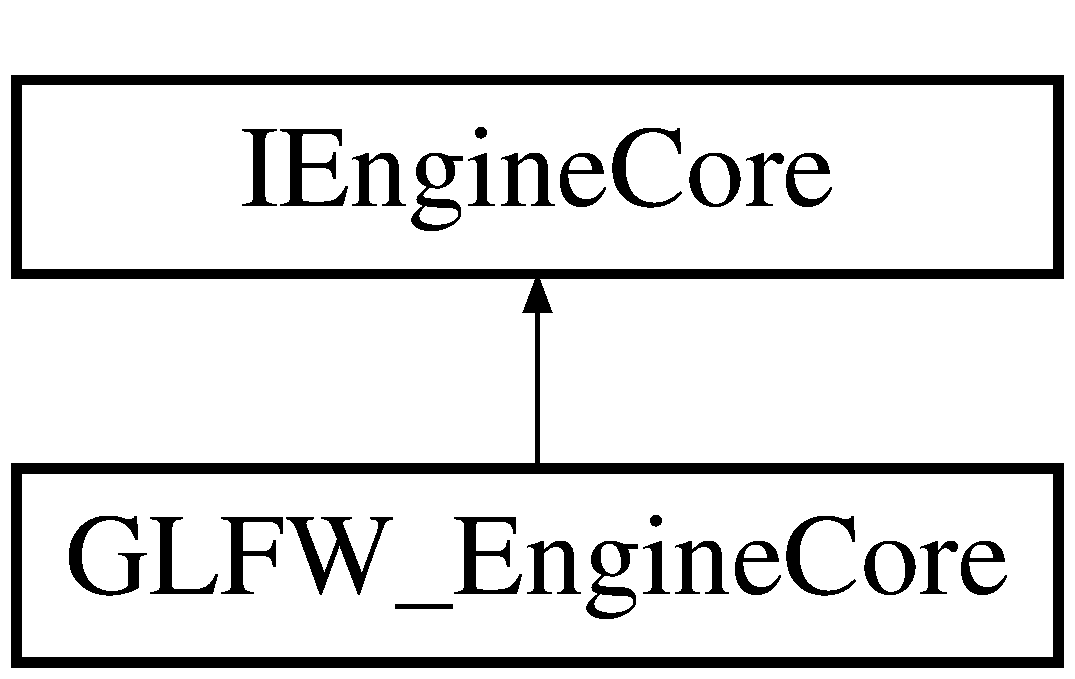
\includegraphics[height=2.000000cm]{class_g_l_f_w___engine_core}
\end{center}
\end{figure}
\subsection*{Public Member Functions}
\begin{DoxyCompactItemize}
\item 
\mbox{\hyperlink{class_g_l_f_w___engine_core_adf17916892982f1103140b22dc1b37be}{$\sim$\+G\+L\+F\+W\+\_\+\+Engine\+Core}} () override
\item 
bool \mbox{\hyperlink{class_g_l_f_w___engine_core_aa786131ec64e7ee6779c3ac1ee8507ce}{init\+Window}} (int width, int height, std\+::string window\+Name) override
\item 
bool \mbox{\hyperlink{class_g_l_f_w___engine_core_adf9266f1a9b5d97992691224f0f20c7b}{run\+Engine}} (\mbox{\hyperlink{class_game}{Game}} \&game) override
\item 
void \mbox{\hyperlink{class_g_l_f_w___engine_core_a6031a54b0978d6e0fd1be3f292c2059f}{render\+Coloured\+Background}} (float r, float g, float b) override
\item 
void \mbox{\hyperlink{class_g_l_f_w___engine_core_a2aba4fb8a635f96fc4057ba841670a29}{set\+Camera}} (const \mbox{\hyperlink{class_camera}{Camera}} $\ast$cam) override
\item 
void \mbox{\hyperlink{class_g_l_f_w___engine_core_a728d1f6ffd1e8526611ab0856db537c0}{draw\+Cube}} (const glm\+::mat4 \&model\+Matrix) override
\item 
void \mbox{\hyperlink{class_g_l_f_w___engine_core_a51f39fe1ceea2f8c47d7c8e89118139d}{draw\+Model}} (\mbox{\hyperlink{class_model}{Model}} $\ast$model, glm\+::mat4 \&model\+Matrix) override
\end{DoxyCompactItemize}


\subsection{Constructor \& Destructor Documentation}
\mbox{\Hypertarget{class_g_l_f_w___engine_core_adf17916892982f1103140b22dc1b37be}\label{class_g_l_f_w___engine_core_adf17916892982f1103140b22dc1b37be}} 
\index{G\+L\+F\+W\+\_\+\+Engine\+Core@{G\+L\+F\+W\+\_\+\+Engine\+Core}!````~G\+L\+F\+W\+\_\+\+Engine\+Core@{$\sim$\+G\+L\+F\+W\+\_\+\+Engine\+Core}}
\index{````~G\+L\+F\+W\+\_\+\+Engine\+Core@{$\sim$\+G\+L\+F\+W\+\_\+\+Engine\+Core}!G\+L\+F\+W\+\_\+\+Engine\+Core@{G\+L\+F\+W\+\_\+\+Engine\+Core}}
\subsubsection{\texorpdfstring{$\sim$\+G\+L\+F\+W\+\_\+\+Engine\+Core()}{~GLFW\_EngineCore()}}
{\footnotesize\ttfamily G\+L\+F\+W\+\_\+\+Engine\+Core\+::$\sim$\+G\+L\+F\+W\+\_\+\+Engine\+Core (\begin{DoxyParamCaption}{ }\end{DoxyParamCaption})\hspace{0.3cm}{\ttfamily [override]}}

Constructor 

\subsection{Member Function Documentation}
\mbox{\Hypertarget{class_g_l_f_w___engine_core_a728d1f6ffd1e8526611ab0856db537c0}\label{class_g_l_f_w___engine_core_a728d1f6ffd1e8526611ab0856db537c0}} 
\index{G\+L\+F\+W\+\_\+\+Engine\+Core@{G\+L\+F\+W\+\_\+\+Engine\+Core}!draw\+Cube@{draw\+Cube}}
\index{draw\+Cube@{draw\+Cube}!G\+L\+F\+W\+\_\+\+Engine\+Core@{G\+L\+F\+W\+\_\+\+Engine\+Core}}
\subsubsection{\texorpdfstring{draw\+Cube()}{drawCube()}}
{\footnotesize\ttfamily void G\+L\+F\+W\+\_\+\+Engine\+Core\+::draw\+Cube (\begin{DoxyParamCaption}\item[{const glm\+::mat4 \&}]{model\+Matrix }\end{DoxyParamCaption})\hspace{0.3cm}{\ttfamily [override]}, {\ttfamily [virtual]}}

Draw\+Cube \+: \mbox{\hyperlink{class_this}{This}} will draw all of the objects in a given scene as a cube. Param One \+: \mbox{\hyperlink{class_the}{The}} model matrix of the object which should be drawn, (position, scale, ext.). 

Implements \mbox{\hyperlink{class_i_engine_core_af24745492d6a7c8bd410a6849fbaf854}{I\+Engine\+Core}}.

\mbox{\Hypertarget{class_g_l_f_w___engine_core_a51f39fe1ceea2f8c47d7c8e89118139d}\label{class_g_l_f_w___engine_core_a51f39fe1ceea2f8c47d7c8e89118139d}} 
\index{G\+L\+F\+W\+\_\+\+Engine\+Core@{G\+L\+F\+W\+\_\+\+Engine\+Core}!draw\+Model@{draw\+Model}}
\index{draw\+Model@{draw\+Model}!G\+L\+F\+W\+\_\+\+Engine\+Core@{G\+L\+F\+W\+\_\+\+Engine\+Core}}
\subsubsection{\texorpdfstring{draw\+Model()}{drawModel()}}
{\footnotesize\ttfamily void G\+L\+F\+W\+\_\+\+Engine\+Core\+::draw\+Model (\begin{DoxyParamCaption}\item[{\mbox{\hyperlink{class_model}{Model}} $\ast$}]{model,  }\item[{glm\+::mat4 \&}]{model\+Matrix }\end{DoxyParamCaption})\hspace{0.3cm}{\ttfamily [override]}, {\ttfamily [virtual]}}

Draw\+Model \+: \mbox{\hyperlink{class_this}{This}} will be used to draw the models into a scene. Param One \+: \mbox{\hyperlink{class_the}{The}} model which should be drawn. Param Two \+: \mbox{\hyperlink{class_the}{The}} model matrix for that model, (position, scale, ext.). 

Implements \mbox{\hyperlink{class_i_engine_core_a454b3f14b3a567852d891c7543edfef7}{I\+Engine\+Core}}.

\mbox{\Hypertarget{class_g_l_f_w___engine_core_aa786131ec64e7ee6779c3ac1ee8507ce}\label{class_g_l_f_w___engine_core_aa786131ec64e7ee6779c3ac1ee8507ce}} 
\index{G\+L\+F\+W\+\_\+\+Engine\+Core@{G\+L\+F\+W\+\_\+\+Engine\+Core}!init\+Window@{init\+Window}}
\index{init\+Window@{init\+Window}!G\+L\+F\+W\+\_\+\+Engine\+Core@{G\+L\+F\+W\+\_\+\+Engine\+Core}}
\subsubsection{\texorpdfstring{init\+Window()}{initWindow()}}
{\footnotesize\ttfamily bool G\+L\+F\+W\+\_\+\+Engine\+Core\+::init\+Window (\begin{DoxyParamCaption}\item[{int}]{width,  }\item[{int}]{height,  }\item[{std\+::string}]{window\+Name }\end{DoxyParamCaption})\hspace{0.3cm}{\ttfamily [override]}, {\ttfamily [virtual]}}

Init\+Window \+: \mbox{\hyperlink{class_this}{This}} will be used to create a window for the game. Param One \+: \mbox{\hyperlink{class_the}{The}} Width of the game window. Param Two \+: \mbox{\hyperlink{class_the}{The}} Height of the game window. Param Three \+: \mbox{\hyperlink{class_the}{The}} Name of the game window. 

Implements \mbox{\hyperlink{class_i_engine_core_a27123704f8f24eefd9cb47aa9986cbf3}{I\+Engine\+Core}}.

\mbox{\Hypertarget{class_g_l_f_w___engine_core_a6031a54b0978d6e0fd1be3f292c2059f}\label{class_g_l_f_w___engine_core_a6031a54b0978d6e0fd1be3f292c2059f}} 
\index{G\+L\+F\+W\+\_\+\+Engine\+Core@{G\+L\+F\+W\+\_\+\+Engine\+Core}!render\+Coloured\+Background@{render\+Coloured\+Background}}
\index{render\+Coloured\+Background@{render\+Coloured\+Background}!G\+L\+F\+W\+\_\+\+Engine\+Core@{G\+L\+F\+W\+\_\+\+Engine\+Core}}
\subsubsection{\texorpdfstring{render\+Coloured\+Background()}{renderColouredBackground()}}
{\footnotesize\ttfamily void G\+L\+F\+W\+\_\+\+Engine\+Core\+::render\+Coloured\+Background (\begin{DoxyParamCaption}\item[{float}]{r,  }\item[{float}]{g,  }\item[{float}]{b }\end{DoxyParamCaption})\hspace{0.3cm}{\ttfamily [override]}, {\ttfamily [virtual]}}

Render\+Coloured\+Background \+: \mbox{\hyperlink{class_this}{This}} will be used to display a colourd background within the game. Param One \+: \mbox{\hyperlink{class_the}{The}} Red value. Param Two \+: \mbox{\hyperlink{class_the}{The}} Green value. Param Three \+: \mbox{\hyperlink{class_the}{The}} Blue value. 

Implements \mbox{\hyperlink{class_i_engine_core_a8f8e0778f04c50b680cdde167cb38e2f}{I\+Engine\+Core}}.

\mbox{\Hypertarget{class_g_l_f_w___engine_core_adf9266f1a9b5d97992691224f0f20c7b}\label{class_g_l_f_w___engine_core_adf9266f1a9b5d97992691224f0f20c7b}} 
\index{G\+L\+F\+W\+\_\+\+Engine\+Core@{G\+L\+F\+W\+\_\+\+Engine\+Core}!run\+Engine@{run\+Engine}}
\index{run\+Engine@{run\+Engine}!G\+L\+F\+W\+\_\+\+Engine\+Core@{G\+L\+F\+W\+\_\+\+Engine\+Core}}
\subsubsection{\texorpdfstring{run\+Engine()}{runEngine()}}
{\footnotesize\ttfamily bool G\+L\+F\+W\+\_\+\+Engine\+Core\+::run\+Engine (\begin{DoxyParamCaption}\item[{\mbox{\hyperlink{class_game}{Game}} \&}]{game }\end{DoxyParamCaption})\hspace{0.3cm}{\ttfamily [override]}, {\ttfamily [virtual]}}

Run\+Engine \+: \mbox{\hyperlink{class_this}{This}} will be used to operate the game loop with the engine core. Param One \+: \mbox{\hyperlink{class_the}{The}} game loop to run. 

Implements \mbox{\hyperlink{class_i_engine_core_ad03940f571ec20ba7427feeca44ace21}{I\+Engine\+Core}}.

\mbox{\Hypertarget{class_g_l_f_w___engine_core_a2aba4fb8a635f96fc4057ba841670a29}\label{class_g_l_f_w___engine_core_a2aba4fb8a635f96fc4057ba841670a29}} 
\index{G\+L\+F\+W\+\_\+\+Engine\+Core@{G\+L\+F\+W\+\_\+\+Engine\+Core}!set\+Camera@{set\+Camera}}
\index{set\+Camera@{set\+Camera}!G\+L\+F\+W\+\_\+\+Engine\+Core@{G\+L\+F\+W\+\_\+\+Engine\+Core}}
\subsubsection{\texorpdfstring{set\+Camera()}{setCamera()}}
{\footnotesize\ttfamily void G\+L\+F\+W\+\_\+\+Engine\+Core\+::set\+Camera (\begin{DoxyParamCaption}\item[{const \mbox{\hyperlink{class_camera}{Camera}} $\ast$}]{cam }\end{DoxyParamCaption})\hspace{0.3cm}{\ttfamily [override]}, {\ttfamily [virtual]}}

Set\+Camera \+: \mbox{\hyperlink{class_this}{This}} will be used to set the camera which will be used to display the scene. Param One \+: \mbox{\hyperlink{class_the}{The}} camera which will be used for the game engine. 

Implements \mbox{\hyperlink{class_i_engine_core_ab2f643ce25708c87b20eecdcbb18b9ac}{I\+Engine\+Core}}.



The documentation for this class was generated from the following file\+:\begin{DoxyCompactItemize}
\item 
Game\+Engine/include/\mbox{\hyperlink{_g_l_f_w___engine_core_8h}{G\+L\+F\+W\+\_\+\+Engine\+Core.\+h}}\end{DoxyCompactItemize}

\hypertarget{class_green_component}{}\section{Green\+Component Class Reference}
\label{class_green_component}\index{Green\+Component@{Green\+Component}}


{\ttfamily \#include $<$Colour\+Component.\+h$>$}

Inheritance diagram for Green\+Component\+:\begin{figure}[H]
\begin{center}
\leavevmode
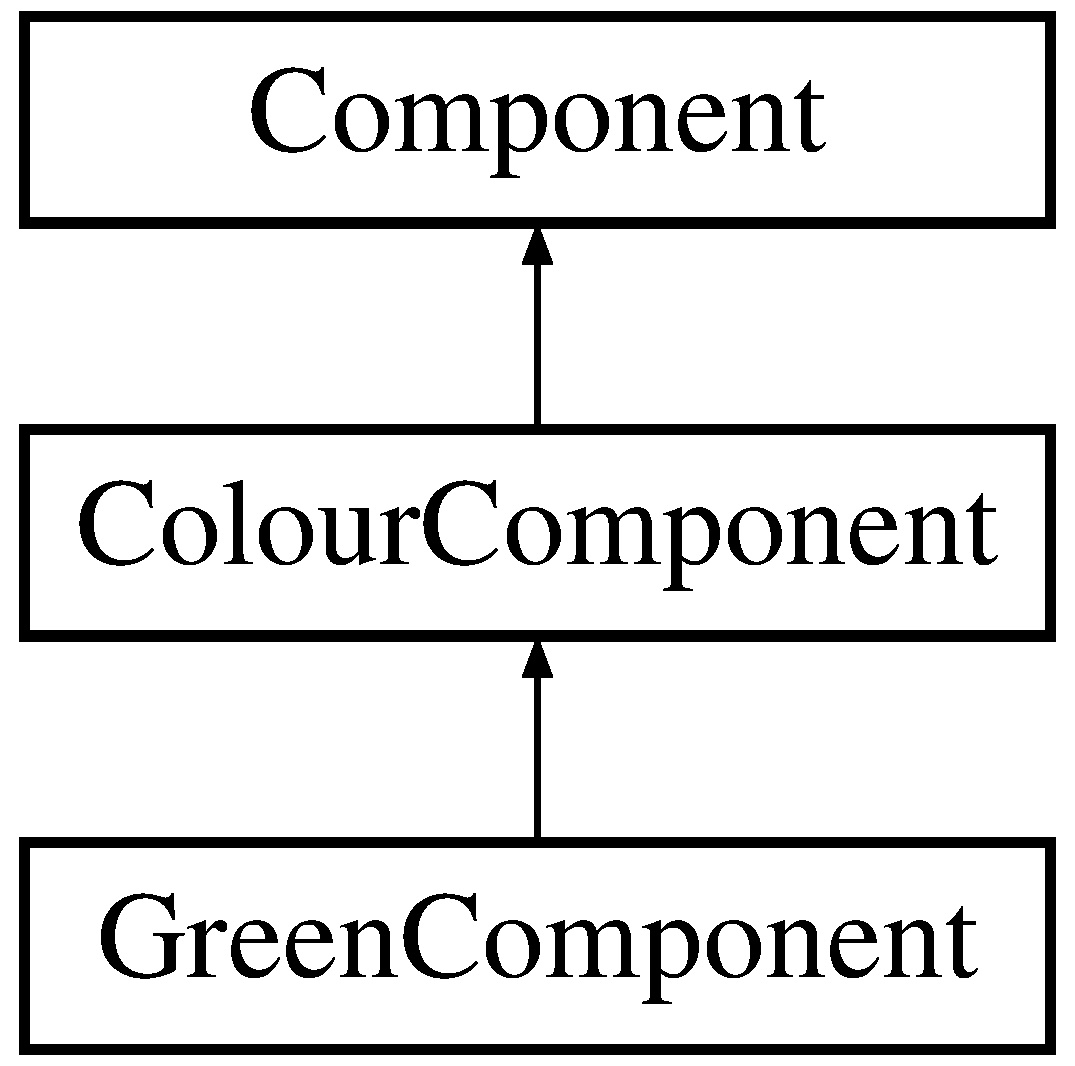
\includegraphics[height=3.000000cm]{class_green_component}
\end{center}
\end{figure}
\subsection*{Additional Inherited Members}


The documentation for this class was generated from the following file\+:\begin{DoxyCompactItemize}
\item 
Game\+Engine/include/\mbox{\hyperlink{_colour_component_8h}{Colour\+Component.\+h}}\end{DoxyCompactItemize}

\hypertarget{class_handles}{}\section{Handles Class Reference}
\label{class_handles}\index{Handles@{Handles}}


\subsection{Detailed Description}
the inputs within the game. 

The documentation for this class was generated from the following file\+:\begin{DoxyCompactItemize}
\item 
Game\+Engine/include/\mbox{\hyperlink{_input_handler_8h}{Input\+Handler.\+h}}\end{DoxyCompactItemize}

\hypertarget{class_i_engine_core}{}\section{I\+Engine\+Core Class Reference}
\label{class_i_engine_core}\index{I\+Engine\+Core@{I\+Engine\+Core}}


{\ttfamily \#include $<$I\+Engine\+Core.\+h$>$}

Inheritance diagram for I\+Engine\+Core\+:\begin{figure}[H]
\begin{center}
\leavevmode
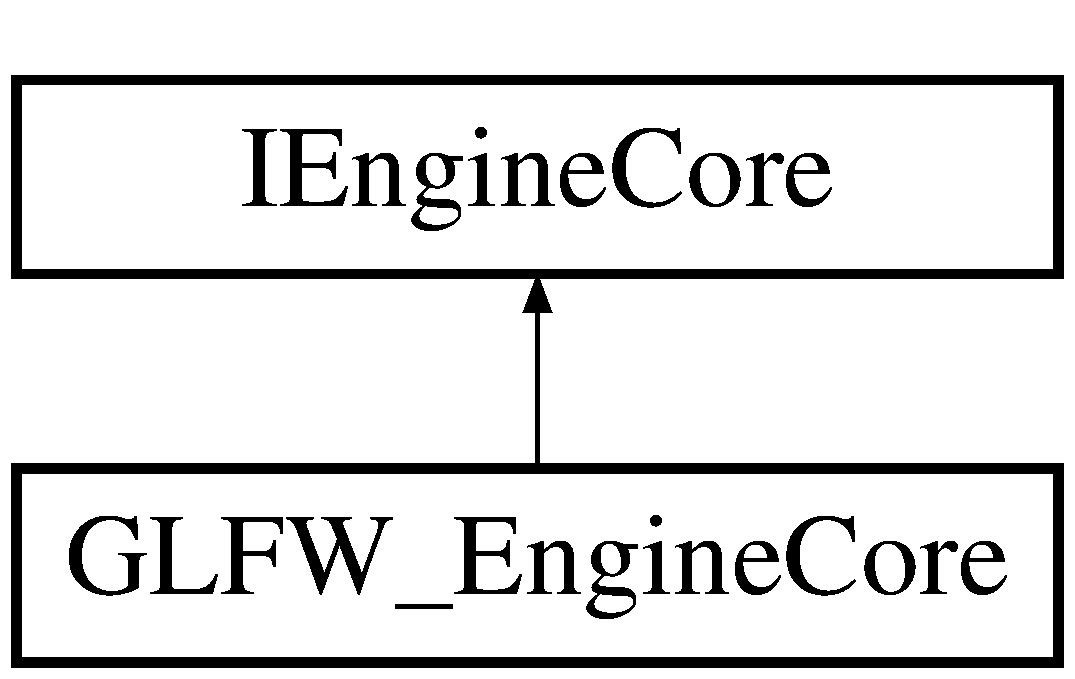
\includegraphics[height=2.000000cm]{class_i_engine_core}
\end{center}
\end{figure}
\subsection*{Public Member Functions}
\begin{DoxyCompactItemize}
\item 
virtual \mbox{\hyperlink{class_i_engine_core_a500720d444543140a1f4f1f80e03d87a}{$\sim$\+I\+Engine\+Core}} ()
\item 
virtual bool \mbox{\hyperlink{class_i_engine_core_a27123704f8f24eefd9cb47aa9986cbf3}{init\+Window}} (int width, int height, std\+::string window\+Name)=0
\item 
virtual bool \mbox{\hyperlink{class_i_engine_core_ad03940f571ec20ba7427feeca44ace21}{run\+Engine}} (\mbox{\hyperlink{class_game}{Game}} \&game)=0
\item 
virtual void \mbox{\hyperlink{class_i_engine_core_a8f8e0778f04c50b680cdde167cb38e2f}{render\+Coloured\+Background}} (float r, float g, float b)=0
\item 
virtual void \mbox{\hyperlink{class_i_engine_core_ab2f643ce25708c87b20eecdcbb18b9ac}{set\+Camera}} (const \mbox{\hyperlink{class_camera}{Camera}} $\ast$cam)=0
\item 
virtual void \mbox{\hyperlink{class_i_engine_core_af24745492d6a7c8bd410a6849fbaf854}{draw\+Cube}} (const glm\+::mat4 \&model\+Matrix)=0
\item 
virtual void \mbox{\hyperlink{class_i_engine_core_a454b3f14b3a567852d891c7543edfef7}{draw\+Model}} (\mbox{\hyperlink{class_model}{Model}} $\ast$model, glm\+::mat4 \&model\+Matrix)=0
\end{DoxyCompactItemize}


\subsection{Constructor \& Destructor Documentation}
\mbox{\Hypertarget{class_i_engine_core_a500720d444543140a1f4f1f80e03d87a}\label{class_i_engine_core_a500720d444543140a1f4f1f80e03d87a}} 
\index{I\+Engine\+Core@{I\+Engine\+Core}!````~I\+Engine\+Core@{$\sim$\+I\+Engine\+Core}}
\index{````~I\+Engine\+Core@{$\sim$\+I\+Engine\+Core}!I\+Engine\+Core@{I\+Engine\+Core}}
\subsubsection{\texorpdfstring{$\sim$\+I\+Engine\+Core()}{~IEngineCore()}}
{\footnotesize\ttfamily virtual I\+Engine\+Core\+::$\sim$\+I\+Engine\+Core (\begin{DoxyParamCaption}{ }\end{DoxyParamCaption})\hspace{0.3cm}{\ttfamily [inline]}, {\ttfamily [virtual]}}

Deconstructor 

\subsection{Member Function Documentation}
\mbox{\Hypertarget{class_i_engine_core_af24745492d6a7c8bd410a6849fbaf854}\label{class_i_engine_core_af24745492d6a7c8bd410a6849fbaf854}} 
\index{I\+Engine\+Core@{I\+Engine\+Core}!draw\+Cube@{draw\+Cube}}
\index{draw\+Cube@{draw\+Cube}!I\+Engine\+Core@{I\+Engine\+Core}}
\subsubsection{\texorpdfstring{draw\+Cube()}{drawCube()}}
{\footnotesize\ttfamily virtual void I\+Engine\+Core\+::draw\+Cube (\begin{DoxyParamCaption}\item[{const glm\+::mat4 \&}]{model\+Matrix }\end{DoxyParamCaption})\hspace{0.3cm}{\ttfamily [pure virtual]}}

Draw\+Cube \+: \mbox{\hyperlink{class_this}{This}} will draw all of the objects in a given scene as a cube. Param One \+: \mbox{\hyperlink{class_the}{The}} model matrix of the object which should be drawn, (position, scale, ext.). 

Implemented in \mbox{\hyperlink{class_g_l_f_w___engine_core_a728d1f6ffd1e8526611ab0856db537c0}{G\+L\+F\+W\+\_\+\+Engine\+Core}}.

\mbox{\Hypertarget{class_i_engine_core_a454b3f14b3a567852d891c7543edfef7}\label{class_i_engine_core_a454b3f14b3a567852d891c7543edfef7}} 
\index{I\+Engine\+Core@{I\+Engine\+Core}!draw\+Model@{draw\+Model}}
\index{draw\+Model@{draw\+Model}!I\+Engine\+Core@{I\+Engine\+Core}}
\subsubsection{\texorpdfstring{draw\+Model()}{drawModel()}}
{\footnotesize\ttfamily virtual void I\+Engine\+Core\+::draw\+Model (\begin{DoxyParamCaption}\item[{\mbox{\hyperlink{class_model}{Model}} $\ast$}]{model,  }\item[{glm\+::mat4 \&}]{model\+Matrix }\end{DoxyParamCaption})\hspace{0.3cm}{\ttfamily [pure virtual]}}

Draw\+Model \+: \mbox{\hyperlink{class_this}{This}} will be used to draw the models into a scene. Param One \+: \mbox{\hyperlink{class_the}{The}} model which should be drawn. Param Two \+: \mbox{\hyperlink{class_the}{The}} model matrix for that model, (position, scale, ext.). 

Implemented in \mbox{\hyperlink{class_g_l_f_w___engine_core_a51f39fe1ceea2f8c47d7c8e89118139d}{G\+L\+F\+W\+\_\+\+Engine\+Core}}.

\mbox{\Hypertarget{class_i_engine_core_a27123704f8f24eefd9cb47aa9986cbf3}\label{class_i_engine_core_a27123704f8f24eefd9cb47aa9986cbf3}} 
\index{I\+Engine\+Core@{I\+Engine\+Core}!init\+Window@{init\+Window}}
\index{init\+Window@{init\+Window}!I\+Engine\+Core@{I\+Engine\+Core}}
\subsubsection{\texorpdfstring{init\+Window()}{initWindow()}}
{\footnotesize\ttfamily virtual bool I\+Engine\+Core\+::init\+Window (\begin{DoxyParamCaption}\item[{int}]{width,  }\item[{int}]{height,  }\item[{std\+::string}]{window\+Name }\end{DoxyParamCaption})\hspace{0.3cm}{\ttfamily [pure virtual]}}

Init\+Window \+: \mbox{\hyperlink{class_this}{This}} will be used to crate the game window. Param One \+: \mbox{\hyperlink{class_the}{The}} width for the game window. Param Two \+: \mbox{\hyperlink{class_the}{The}} height for the game window. Param Three \+: \mbox{\hyperlink{class_the}{The}} name for the game window. 

Implemented in \mbox{\hyperlink{class_g_l_f_w___engine_core_aa786131ec64e7ee6779c3ac1ee8507ce}{G\+L\+F\+W\+\_\+\+Engine\+Core}}.

\mbox{\Hypertarget{class_i_engine_core_a8f8e0778f04c50b680cdde167cb38e2f}\label{class_i_engine_core_a8f8e0778f04c50b680cdde167cb38e2f}} 
\index{I\+Engine\+Core@{I\+Engine\+Core}!render\+Coloured\+Background@{render\+Coloured\+Background}}
\index{render\+Coloured\+Background@{render\+Coloured\+Background}!I\+Engine\+Core@{I\+Engine\+Core}}
\subsubsection{\texorpdfstring{render\+Coloured\+Background()}{renderColouredBackground()}}
{\footnotesize\ttfamily virtual void I\+Engine\+Core\+::render\+Coloured\+Background (\begin{DoxyParamCaption}\item[{float}]{r,  }\item[{float}]{g,  }\item[{float}]{b }\end{DoxyParamCaption})\hspace{0.3cm}{\ttfamily [pure virtual]}}

Render\+Coloured\+Background \+: \mbox{\hyperlink{class_this}{This}} will be used to display a colourd background within the game. Param One \+: \mbox{\hyperlink{class_the}{The}} Red value. Param Two \+: \mbox{\hyperlink{class_the}{The}} Green value. Param Three \+: \mbox{\hyperlink{class_the}{The}} Blue value. 

Implemented in \mbox{\hyperlink{class_g_l_f_w___engine_core_a6031a54b0978d6e0fd1be3f292c2059f}{G\+L\+F\+W\+\_\+\+Engine\+Core}}.

\mbox{\Hypertarget{class_i_engine_core_ad03940f571ec20ba7427feeca44ace21}\label{class_i_engine_core_ad03940f571ec20ba7427feeca44ace21}} 
\index{I\+Engine\+Core@{I\+Engine\+Core}!run\+Engine@{run\+Engine}}
\index{run\+Engine@{run\+Engine}!I\+Engine\+Core@{I\+Engine\+Core}}
\subsubsection{\texorpdfstring{run\+Engine()}{runEngine()}}
{\footnotesize\ttfamily virtual bool I\+Engine\+Core\+::run\+Engine (\begin{DoxyParamCaption}\item[{\mbox{\hyperlink{class_game}{Game}} \&}]{game }\end{DoxyParamCaption})\hspace{0.3cm}{\ttfamily [pure virtual]}}

Run\+Engine \+: \mbox{\hyperlink{class_this}{This}} will be used to run the main game loop. Param One \+: \mbox{\hyperlink{class_the}{The}} game to run. 

Implemented in \mbox{\hyperlink{class_g_l_f_w___engine_core_adf9266f1a9b5d97992691224f0f20c7b}{G\+L\+F\+W\+\_\+\+Engine\+Core}}.

\mbox{\Hypertarget{class_i_engine_core_ab2f643ce25708c87b20eecdcbb18b9ac}\label{class_i_engine_core_ab2f643ce25708c87b20eecdcbb18b9ac}} 
\index{I\+Engine\+Core@{I\+Engine\+Core}!set\+Camera@{set\+Camera}}
\index{set\+Camera@{set\+Camera}!I\+Engine\+Core@{I\+Engine\+Core}}
\subsubsection{\texorpdfstring{set\+Camera()}{setCamera()}}
{\footnotesize\ttfamily virtual void I\+Engine\+Core\+::set\+Camera (\begin{DoxyParamCaption}\item[{const \mbox{\hyperlink{class_camera}{Camera}} $\ast$}]{cam }\end{DoxyParamCaption})\hspace{0.3cm}{\ttfamily [pure virtual]}}

Set\+Camera \+: \mbox{\hyperlink{class_this}{This}} will be used to set the camera which will be used to display the scene. Param One \+: \mbox{\hyperlink{class_the}{The}} camera which will be used for the game engine. 

Implemented in \mbox{\hyperlink{class_g_l_f_w___engine_core_a2aba4fb8a635f96fc4057ba841670a29}{G\+L\+F\+W\+\_\+\+Engine\+Core}}.



The documentation for this class was generated from the following file\+:\begin{DoxyCompactItemize}
\item 
Game\+Engine/include/\mbox{\hyperlink{_i_engine_core_8h}{I\+Engine\+Core.\+h}}\end{DoxyCompactItemize}

\hypertarget{class_input_command}{}\section{Input\+Command Class Reference}
\label{class_input_command}\index{Input\+Command@{Input\+Command}}


{\ttfamily \#include $<$Input\+Handler.\+h$>$}

Inheritance diagram for Input\+Command\+:\begin{figure}[H]
\begin{center}
\leavevmode
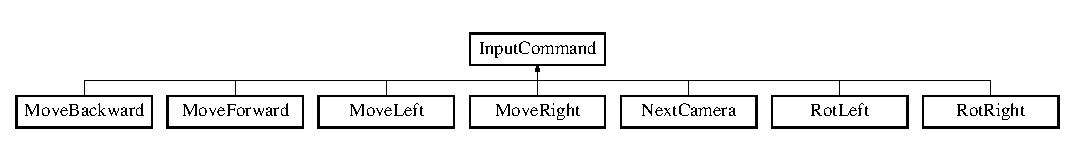
\includegraphics[height=1.481482cm]{class_input_command}
\end{center}
\end{figure}
\subsection*{Public Member Functions}
\begin{DoxyCompactItemize}
\item 
virtual \mbox{\hyperlink{class_input_command_a203385c2bfacb53d17ac5749ee274dc0}{$\sim$\+Input\+Command}} ()
\item 
virtual void \mbox{\hyperlink{class_input_command_a14fb500713d0813165f0c864d47553a0}{execute}} (\mbox{\hyperlink{class_game_object}{Game\+Object}} \&player\+Background)=0
\item 
virtual const char $\ast$ \mbox{\hyperlink{class_input_command_aa28e1877f850c588b5a2dff8d41eb627}{m\+\_\+\+Class\+Name}} ()=0
\end{DoxyCompactItemize}


\subsection{Constructor \& Destructor Documentation}
\mbox{\Hypertarget{class_input_command_a203385c2bfacb53d17ac5749ee274dc0}\label{class_input_command_a203385c2bfacb53d17ac5749ee274dc0}} 
\index{Input\+Command@{Input\+Command}!````~Input\+Command@{$\sim$\+Input\+Command}}
\index{````~Input\+Command@{$\sim$\+Input\+Command}!Input\+Command@{Input\+Command}}
\subsubsection{\texorpdfstring{$\sim$\+Input\+Command()}{~InputCommand()}}
{\footnotesize\ttfamily virtual Input\+Command\+::$\sim$\+Input\+Command (\begin{DoxyParamCaption}{ }\end{DoxyParamCaption})\hspace{0.3cm}{\ttfamily [inline]}, {\ttfamily [virtual]}}

Deconstructor 

\subsection{Member Function Documentation}
\mbox{\Hypertarget{class_input_command_a14fb500713d0813165f0c864d47553a0}\label{class_input_command_a14fb500713d0813165f0c864d47553a0}} 
\index{Input\+Command@{Input\+Command}!execute@{execute}}
\index{execute@{execute}!Input\+Command@{Input\+Command}}
\subsubsection{\texorpdfstring{execute()}{execute()}}
{\footnotesize\ttfamily virtual void Input\+Command\+::execute (\begin{DoxyParamCaption}\item[{\mbox{\hyperlink{class_game_object}{Game\+Object}} \&}]{player\+Background }\end{DoxyParamCaption})\hspace{0.3cm}{\ttfamily [pure virtual]}}

Execute \+: \mbox{\hyperlink{class_this}{This}} will be used to run code from a key press. \mbox{\Hypertarget{class_input_command_aa28e1877f850c588b5a2dff8d41eb627}\label{class_input_command_aa28e1877f850c588b5a2dff8d41eb627}} 
\index{Input\+Command@{Input\+Command}!m\+\_\+\+Class\+Name@{m\+\_\+\+Class\+Name}}
\index{m\+\_\+\+Class\+Name@{m\+\_\+\+Class\+Name}!Input\+Command@{Input\+Command}}
\subsubsection{\texorpdfstring{m\+\_\+\+Class\+Name()}{m\_ClassName()}}
{\footnotesize\ttfamily virtual const char$\ast$ Input\+Command\+::m\+\_\+\+Class\+Name (\begin{DoxyParamCaption}{ }\end{DoxyParamCaption})\hspace{0.3cm}{\ttfamily [pure virtual]}}

Class\+Name \+: \mbox{\hyperlink{class_this}{This}} will be used to help load and output this action. 

The documentation for this class was generated from the following file\+:\begin{DoxyCompactItemize}
\item 
Game\+Engine/include/\mbox{\hyperlink{_input_handler_8h}{Input\+Handler.\+h}}\end{DoxyCompactItemize}

\hypertarget{struct_input_handler}{}\section{Input\+Handler Struct Reference}
\label{struct_input_handler}\index{Input\+Handler@{Input\+Handler}}


{\ttfamily \#include $<$Input\+Handler.\+h$>$}

\subsection*{Public Member Functions}
\begin{DoxyCompactItemize}
\item 
\mbox{\hyperlink{struct_input_handler_a951e34a63d07195f594b1469a1e0b859}{Input\+Handler}} (\mbox{\hyperlink{class_game_manager}{Game\+Manager}} $\ast$game\+Manager)
\item 
\mbox{\hyperlink{struct_input_handler_ac1f7efb54b34d433d6ffba62627452b6}{$\sim$\+Input\+Handler}} ()
\item 
void \mbox{\hyperlink{struct_input_handler_ae8150d9263151be0d480a382f2c16b02}{m\+\_\+\+Load\+Config}} ()
\item 
void \mbox{\hyperlink{struct_input_handler_aa133e6d963446578ab282095ca5df05a}{m\+\_\+\+Output\+Config}} ()
\item 
virtual const char $\ast$ \mbox{\hyperlink{struct_input_handler_a4e77e8e4824b8287ae3a5d1af732677f}{m\+\_\+\+Class\+Name}} ()
\item 
void \mbox{\hyperlink{struct_input_handler_a250b665d3a9bc35bd8d6b544266e4faf}{handle\+Inputs}} (const std\+::vector$<$ bool $>$ \&key\+Buffer)
\end{DoxyCompactItemize}
\subsection*{Public Attributes}
\begin{DoxyCompactItemize}
\item 
\mbox{\hyperlink{class_game_object}{Game\+Object}} $\ast$ \mbox{\hyperlink{struct_input_handler_a02162590271ed44ae87ce77e89023026}{m\+\_\+player\+Cube}}
\item 
\mbox{\hyperlink{class_game_manager}{Game\+Manager}} $\ast$ \mbox{\hyperlink{struct_input_handler_ae2a439c9a0559ac885a1322d83cfce4b}{m\+\_\+\+Game\+Manager}}
\item 
std\+::map$<$ int, \mbox{\hyperlink{class_input_command}{Input\+Command}} $\ast$ $>$ \mbox{\hyperlink{struct_input_handler_abe853597d11b94e0668c8db6638a0548}{m\+\_\+control\+Mapping}}
\end{DoxyCompactItemize}


\subsection{Constructor \& Destructor Documentation}
\mbox{\Hypertarget{struct_input_handler_a951e34a63d07195f594b1469a1e0b859}\label{struct_input_handler_a951e34a63d07195f594b1469a1e0b859}} 
\index{Input\+Handler@{Input\+Handler}!Input\+Handler@{Input\+Handler}}
\index{Input\+Handler@{Input\+Handler}!Input\+Handler@{Input\+Handler}}
\subsubsection{\texorpdfstring{Input\+Handler()}{InputHandler()}}
{\footnotesize\ttfamily Input\+Handler\+::\+Input\+Handler (\begin{DoxyParamCaption}\item[{\mbox{\hyperlink{class_game_manager}{Game\+Manager}} $\ast$}]{game\+Manager }\end{DoxyParamCaption})\hspace{0.3cm}{\ttfamily [inline]}}

Constructor Param One \+: A pointer to the player object. \mbox{\Hypertarget{struct_input_handler_ac1f7efb54b34d433d6ffba62627452b6}\label{struct_input_handler_ac1f7efb54b34d433d6ffba62627452b6}} 
\index{Input\+Handler@{Input\+Handler}!````~Input\+Handler@{$\sim$\+Input\+Handler}}
\index{````~Input\+Handler@{$\sim$\+Input\+Handler}!Input\+Handler@{Input\+Handler}}
\subsubsection{\texorpdfstring{$\sim$\+Input\+Handler()}{~InputHandler()}}
{\footnotesize\ttfamily Input\+Handler\+::$\sim$\+Input\+Handler (\begin{DoxyParamCaption}{ }\end{DoxyParamCaption})\hspace{0.3cm}{\ttfamily [inline]}}

Deconstructor 

\subsection{Member Function Documentation}
\mbox{\Hypertarget{struct_input_handler_a250b665d3a9bc35bd8d6b544266e4faf}\label{struct_input_handler_a250b665d3a9bc35bd8d6b544266e4faf}} 
\index{Input\+Handler@{Input\+Handler}!handle\+Inputs@{handle\+Inputs}}
\index{handle\+Inputs@{handle\+Inputs}!Input\+Handler@{Input\+Handler}}
\subsubsection{\texorpdfstring{handle\+Inputs()}{handleInputs()}}
{\footnotesize\ttfamily void Input\+Handler\+::handle\+Inputs (\begin{DoxyParamCaption}\item[{const std\+::vector$<$ bool $>$ \&}]{key\+Buffer }\end{DoxyParamCaption})\hspace{0.3cm}{\ttfamily [inline]}}

Handle\+Inputs \+: \mbox{\hyperlink{class_this}{This}} will use a list of keys pressed this frame and activate thir related functions. Param One \+: A vector of keys pressed. \mbox{\Hypertarget{struct_input_handler_a4e77e8e4824b8287ae3a5d1af732677f}\label{struct_input_handler_a4e77e8e4824b8287ae3a5d1af732677f}} 
\index{Input\+Handler@{Input\+Handler}!m\+\_\+\+Class\+Name@{m\+\_\+\+Class\+Name}}
\index{m\+\_\+\+Class\+Name@{m\+\_\+\+Class\+Name}!Input\+Handler@{Input\+Handler}}
\subsubsection{\texorpdfstring{m\+\_\+\+Class\+Name()}{m\_ClassName()}}
{\footnotesize\ttfamily virtual const char$\ast$ Input\+Handler\+::m\+\_\+\+Class\+Name (\begin{DoxyParamCaption}{ }\end{DoxyParamCaption})\hspace{0.3cm}{\ttfamily [inline]}, {\ttfamily [virtual]}}

Class\+Name \+: \mbox{\hyperlink{class_this}{This}} will beused to get the name of the class, used for the reading/writing to the config file. \mbox{\Hypertarget{struct_input_handler_ae8150d9263151be0d480a382f2c16b02}\label{struct_input_handler_ae8150d9263151be0d480a382f2c16b02}} 
\index{Input\+Handler@{Input\+Handler}!m\+\_\+\+Load\+Config@{m\+\_\+\+Load\+Config}}
\index{m\+\_\+\+Load\+Config@{m\+\_\+\+Load\+Config}!Input\+Handler@{Input\+Handler}}
\subsubsection{\texorpdfstring{m\+\_\+\+Load\+Config()}{m\_LoadConfig()}}
{\footnotesize\ttfamily void Input\+Handler\+::m\+\_\+\+Load\+Config (\begin{DoxyParamCaption}{ }\end{DoxyParamCaption})\hspace{0.3cm}{\ttfamily [inline]}}

Load\+Config \+: \mbox{\hyperlink{class_this}{This}} will be used to read the config file for the game and adjust the key commands used. \mbox{\Hypertarget{struct_input_handler_aa133e6d963446578ab282095ca5df05a}\label{struct_input_handler_aa133e6d963446578ab282095ca5df05a}} 
\index{Input\+Handler@{Input\+Handler}!m\+\_\+\+Output\+Config@{m\+\_\+\+Output\+Config}}
\index{m\+\_\+\+Output\+Config@{m\+\_\+\+Output\+Config}!Input\+Handler@{Input\+Handler}}
\subsubsection{\texorpdfstring{m\+\_\+\+Output\+Config()}{m\_OutputConfig()}}
{\footnotesize\ttfamily void Input\+Handler\+::m\+\_\+\+Output\+Config (\begin{DoxyParamCaption}{ }\end{DoxyParamCaption})\hspace{0.3cm}{\ttfamily [inline]}}

Output\+Config \+: \mbox{\hyperlink{class_this}{This}} will write the current key commands for the engine to a config file within assets. 

\subsection{Member Data Documentation}
\mbox{\Hypertarget{struct_input_handler_abe853597d11b94e0668c8db6638a0548}\label{struct_input_handler_abe853597d11b94e0668c8db6638a0548}} 
\index{Input\+Handler@{Input\+Handler}!m\+\_\+control\+Mapping@{m\+\_\+control\+Mapping}}
\index{m\+\_\+control\+Mapping@{m\+\_\+control\+Mapping}!Input\+Handler@{Input\+Handler}}
\subsubsection{\texorpdfstring{m\+\_\+control\+Mapping}{m\_controlMapping}}
{\footnotesize\ttfamily std\+::map$<$int, \mbox{\hyperlink{class_input_command}{Input\+Command}}$\ast$$>$ Input\+Handler\+::m\+\_\+control\+Mapping}

\mbox{\Hypertarget{struct_input_handler_ae2a439c9a0559ac885a1322d83cfce4b}\label{struct_input_handler_ae2a439c9a0559ac885a1322d83cfce4b}} 
\index{Input\+Handler@{Input\+Handler}!m\+\_\+\+Game\+Manager@{m\+\_\+\+Game\+Manager}}
\index{m\+\_\+\+Game\+Manager@{m\+\_\+\+Game\+Manager}!Input\+Handler@{Input\+Handler}}
\subsubsection{\texorpdfstring{m\+\_\+\+Game\+Manager}{m\_GameManager}}
{\footnotesize\ttfamily \mbox{\hyperlink{class_game_manager}{Game\+Manager}}$\ast$ Input\+Handler\+::m\+\_\+\+Game\+Manager}

\mbox{\Hypertarget{struct_input_handler_a02162590271ed44ae87ce77e89023026}\label{struct_input_handler_a02162590271ed44ae87ce77e89023026}} 
\index{Input\+Handler@{Input\+Handler}!m\+\_\+player\+Cube@{m\+\_\+player\+Cube}}
\index{m\+\_\+player\+Cube@{m\+\_\+player\+Cube}!Input\+Handler@{Input\+Handler}}
\subsubsection{\texorpdfstring{m\+\_\+player\+Cube}{m\_playerCube}}
{\footnotesize\ttfamily \mbox{\hyperlink{class_game_object}{Game\+Object}}$\ast$ Input\+Handler\+::m\+\_\+player\+Cube}



The documentation for this struct was generated from the following file\+:\begin{DoxyCompactItemize}
\item 
Game\+Engine/include/\mbox{\hyperlink{_input_handler_8h}{Input\+Handler.\+h}}\end{DoxyCompactItemize}

\hypertarget{class_mesh}{}\section{Mesh Class Reference}
\label{class_mesh}\index{Mesh@{Mesh}}


{\ttfamily \#include $<$Mesh.\+h$>$}

\subsection*{Public Member Functions}
\begin{DoxyCompactItemize}
\item 
\mbox{\hyperlink{class_mesh_a2d6c71adb66e5f270cee7a60c4e23018}{Mesh}} (vector$<$ \mbox{\hyperlink{struct_vertex}{Vertex}} $>$ \mbox{\hyperlink{class_mesh_abe5c05c224e47ba1e8b6393759798a9b}{vertices}}, vector$<$ unsigned int $>$ \mbox{\hyperlink{class_mesh_a464d9a1d7e7a4f67321dffc1e8b44b7d}{indices}}, vector$<$ \mbox{\hyperlink{struct_texture}{Texture}} $>$ \mbox{\hyperlink{class_mesh_a09bf4e8307bf7717c56501ca6293c6c0}{textures}})
\item 
void \mbox{\hyperlink{class_mesh_a9a6ec018bec776cb7b31fb8433c8a7e7}{render}} (const unsigned int shader\+Program)
\end{DoxyCompactItemize}
\subsection*{Public Attributes}
\begin{DoxyCompactItemize}
\item 
vector$<$ \mbox{\hyperlink{struct_vertex}{Vertex}} $>$ \mbox{\hyperlink{class_mesh_abe5c05c224e47ba1e8b6393759798a9b}{vertices}}
\item 
vector$<$ unsigned int $>$ \mbox{\hyperlink{class_mesh_a464d9a1d7e7a4f67321dffc1e8b44b7d}{indices}}
\item 
vector$<$ \mbox{\hyperlink{struct_texture}{Texture}} $>$ \mbox{\hyperlink{class_mesh_a09bf4e8307bf7717c56501ca6293c6c0}{textures}}
\item 
unsigned int \mbox{\hyperlink{class_mesh_a79afa055e485fb65b1a7aa5b8eda2940}{V\+AO}}
\end{DoxyCompactItemize}


\subsection{Constructor \& Destructor Documentation}
\mbox{\Hypertarget{class_mesh_a2d6c71adb66e5f270cee7a60c4e23018}\label{class_mesh_a2d6c71adb66e5f270cee7a60c4e23018}} 
\index{Mesh@{Mesh}!Mesh@{Mesh}}
\index{Mesh@{Mesh}!Mesh@{Mesh}}
\subsubsection{\texorpdfstring{Mesh()}{Mesh()}}
{\footnotesize\ttfamily Mesh\+::\+Mesh (\begin{DoxyParamCaption}\item[{vector$<$ \mbox{\hyperlink{struct_vertex}{Vertex}} $>$}]{vertices,  }\item[{vector$<$ unsigned int $>$}]{indices,  }\item[{vector$<$ \mbox{\hyperlink{struct_texture}{Texture}} $>$}]{textures }\end{DoxyParamCaption})}

Constructor Param One \+: A list of verices used by the model. Param Two \+: A list of indices used by the model. Param Three \+: \mbox{\hyperlink{class_the}{The}} list of textures for the model. 

\subsection{Member Function Documentation}
\mbox{\Hypertarget{class_mesh_a9a6ec018bec776cb7b31fb8433c8a7e7}\label{class_mesh_a9a6ec018bec776cb7b31fb8433c8a7e7}} 
\index{Mesh@{Mesh}!render@{render}}
\index{render@{render}!Mesh@{Mesh}}
\subsubsection{\texorpdfstring{render()}{render()}}
{\footnotesize\ttfamily void Mesh\+::render (\begin{DoxyParamCaption}\item[{const unsigned int}]{shader\+Program }\end{DoxyParamCaption})}

Render \+: Render the mesh with a given shader program Param One \+: \mbox{\hyperlink{class_the}{The}} current shader program being used. 

\subsection{Member Data Documentation}
\mbox{\Hypertarget{class_mesh_a464d9a1d7e7a4f67321dffc1e8b44b7d}\label{class_mesh_a464d9a1d7e7a4f67321dffc1e8b44b7d}} 
\index{Mesh@{Mesh}!indices@{indices}}
\index{indices@{indices}!Mesh@{Mesh}}
\subsubsection{\texorpdfstring{indices}{indices}}
{\footnotesize\ttfamily vector$<$unsigned int$>$ Mesh\+::indices}

\mbox{\Hypertarget{class_mesh_a09bf4e8307bf7717c56501ca6293c6c0}\label{class_mesh_a09bf4e8307bf7717c56501ca6293c6c0}} 
\index{Mesh@{Mesh}!textures@{textures}}
\index{textures@{textures}!Mesh@{Mesh}}
\subsubsection{\texorpdfstring{textures}{textures}}
{\footnotesize\ttfamily vector$<$\mbox{\hyperlink{struct_texture}{Texture}}$>$ Mesh\+::textures}

\mbox{\Hypertarget{class_mesh_a79afa055e485fb65b1a7aa5b8eda2940}\label{class_mesh_a79afa055e485fb65b1a7aa5b8eda2940}} 
\index{Mesh@{Mesh}!V\+AO@{V\+AO}}
\index{V\+AO@{V\+AO}!Mesh@{Mesh}}
\subsubsection{\texorpdfstring{V\+AO}{VAO}}
{\footnotesize\ttfamily unsigned int Mesh\+::\+V\+AO}

\mbox{\Hypertarget{class_mesh_abe5c05c224e47ba1e8b6393759798a9b}\label{class_mesh_abe5c05c224e47ba1e8b6393759798a9b}} 
\index{Mesh@{Mesh}!vertices@{vertices}}
\index{vertices@{vertices}!Mesh@{Mesh}}
\subsubsection{\texorpdfstring{vertices}{vertices}}
{\footnotesize\ttfamily vector$<$\mbox{\hyperlink{struct_vertex}{Vertex}}$>$ Mesh\+::vertices}



The documentation for this class was generated from the following file\+:\begin{DoxyCompactItemize}
\item 
Game\+Engine/include/\mbox{\hyperlink{_mesh_8h}{Mesh.\+h}}\end{DoxyCompactItemize}

\hypertarget{class_model}{}\section{Model Class Reference}
\label{class_model}\index{Model@{Model}}


{\ttfamily \#include $<$Model.\+h$>$}

\subsection*{Public Member Functions}
\begin{DoxyCompactItemize}
\item 
\mbox{\hyperlink{class_model_a4a90abd11a1c4e47f1b704e28e147dfb}{Model}} (string filepath)
\item 
void \mbox{\hyperlink{class_model_a0885da76930d0f3b919eaa10ae08e8ab}{render}} (const unsigned int shader\+Program)
\end{DoxyCompactItemize}
\subsection*{Static Public Member Functions}
\begin{DoxyCompactItemize}
\item 
static unsigned int \mbox{\hyperlink{class_model_a16c263d87f6368d21d5ab255468c2c90}{Texture\+From\+File}} (const char $\ast$filepath, const string \&directory, bool gamma=false)
\end{DoxyCompactItemize}


\subsection{Constructor \& Destructor Documentation}
\mbox{\Hypertarget{class_model_a4a90abd11a1c4e47f1b704e28e147dfb}\label{class_model_a4a90abd11a1c4e47f1b704e28e147dfb}} 
\index{Model@{Model}!Model@{Model}}
\index{Model@{Model}!Model@{Model}}
\subsubsection{\texorpdfstring{Model()}{Model()}}
{\footnotesize\ttfamily Model\+::\+Model (\begin{DoxyParamCaption}\item[{string}]{filepath }\end{DoxyParamCaption})}

Constructor Param One \+: \mbox{\hyperlink{class_the}{The}} file path to find the model. 

\subsection{Member Function Documentation}
\mbox{\Hypertarget{class_model_a0885da76930d0f3b919eaa10ae08e8ab}\label{class_model_a0885da76930d0f3b919eaa10ae08e8ab}} 
\index{Model@{Model}!render@{render}}
\index{render@{render}!Model@{Model}}
\subsubsection{\texorpdfstring{render()}{render()}}
{\footnotesize\ttfamily void Model\+::render (\begin{DoxyParamCaption}\item[{const unsigned int}]{shader\+Program }\end{DoxyParamCaption})}

Render \+: \mbox{\hyperlink{class_this}{This}} will be usesd to render the model in the scene. Param One \+: \mbox{\hyperlink{class_the}{The}} current shader program used by the game engine. \mbox{\Hypertarget{class_model_a16c263d87f6368d21d5ab255468c2c90}\label{class_model_a16c263d87f6368d21d5ab255468c2c90}} 
\index{Model@{Model}!Texture\+From\+File@{Texture\+From\+File}}
\index{Texture\+From\+File@{Texture\+From\+File}!Model@{Model}}
\subsubsection{\texorpdfstring{Texture\+From\+File()}{TextureFromFile()}}
{\footnotesize\ttfamily static unsigned int Model\+::\+Texture\+From\+File (\begin{DoxyParamCaption}\item[{const char $\ast$}]{filepath,  }\item[{const string \&}]{directory,  }\item[{bool}]{gamma = {\ttfamily false} }\end{DoxyParamCaption})\hspace{0.3cm}{\ttfamily [static]}}

Texture\+From\+File \+: \mbox{\hyperlink{class_this}{This}} will be used to load a model\textquotesingle{}s texture from a file. Param One \+: \mbox{\hyperlink{class_the}{The}} name of the file. Param Two \+: \mbox{\hyperlink{class_the}{The}} location where to find the file. Param Three \+: \mbox{\hyperlink{class_the}{The}} gamma in the texture. 

The documentation for this class was generated from the following file\+:\begin{DoxyCompactItemize}
\item 
Game\+Engine/include/\mbox{\hyperlink{_model_8h}{Model.\+h}}\end{DoxyCompactItemize}

\hypertarget{class_model_component}{}\section{Model\+Component Class Reference}
\label{class_model_component}\index{Model\+Component@{Model\+Component}}


{\ttfamily \#include $<$Model\+Component.\+h$>$}

Inheritance diagram for Model\+Component\+:\begin{figure}[H]
\begin{center}
\leavevmode
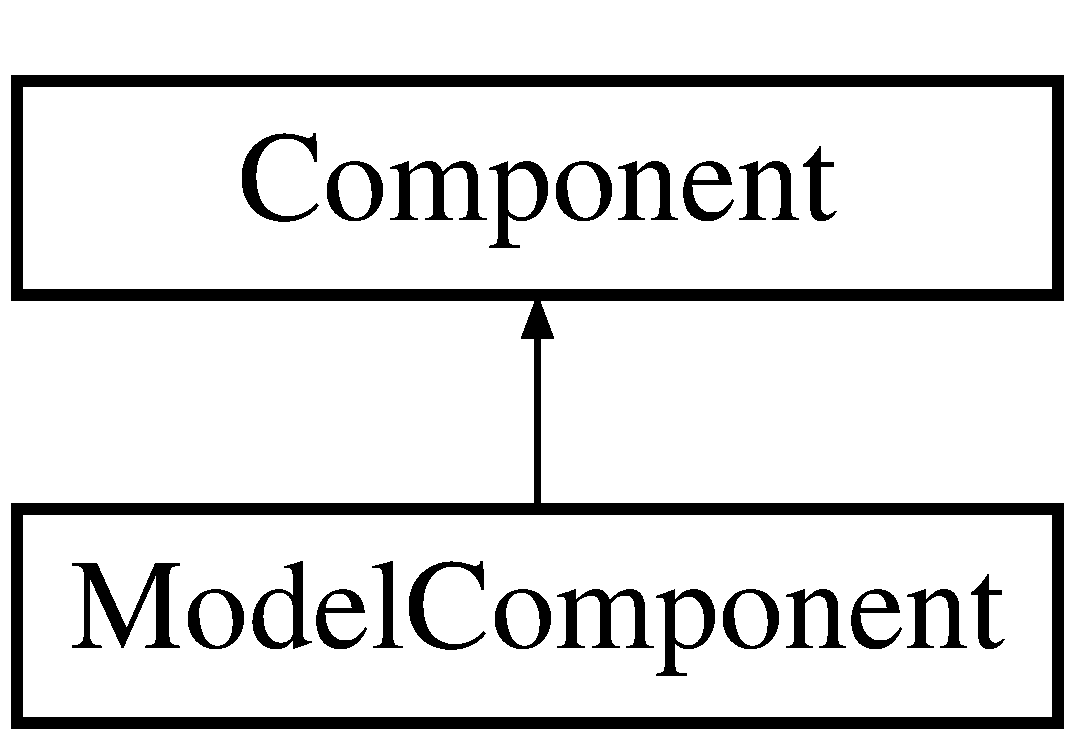
\includegraphics[height=2.000000cm]{class_model_component}
\end{center}
\end{figure}
\subsection*{Public Member Functions}
\begin{DoxyCompactItemize}
\item 
\mbox{\hyperlink{class_model_component_a17f51d0e24fedfc6e7dd3633046665e4}{Model\+Component}} (\mbox{\hyperlink{class_model}{Model}} $\ast$target\+Model)
\item 
\mbox{\hyperlink{class_model_component_a6d490d6a2fdf66ad13ed8adcc39ec611}{$\sim$\+Model\+Component}} ()
\item 
void \mbox{\hyperlink{class_model_component_a5def59776319943854fb5da3dc515051}{On\+Update}} (float dt) override
\item 
void \mbox{\hyperlink{class_model_component_a48d6170e857f323839039ce54e9418e1}{On\+Message}} (const std\+::string m) override
\end{DoxyCompactItemize}
\subsection*{Public Attributes}
\begin{DoxyCompactItemize}
\item 
\mbox{\hyperlink{class_model}{Model}} $\ast$ \mbox{\hyperlink{class_model_component_afff2101b1cdbf6a8339fa151bcc8b6e0}{m\+\_\+\+This\+Model}}
\end{DoxyCompactItemize}


\subsection{Constructor \& Destructor Documentation}
\mbox{\Hypertarget{class_model_component_a17f51d0e24fedfc6e7dd3633046665e4}\label{class_model_component_a17f51d0e24fedfc6e7dd3633046665e4}} 
\index{Model\+Component@{Model\+Component}!Model\+Component@{Model\+Component}}
\index{Model\+Component@{Model\+Component}!Model\+Component@{Model\+Component}}
\subsubsection{\texorpdfstring{Model\+Component()}{ModelComponent()}}
{\footnotesize\ttfamily Model\+Component\+::\+Model\+Component (\begin{DoxyParamCaption}\item[{\mbox{\hyperlink{class_model}{Model}} $\ast$}]{target\+Model }\end{DoxyParamCaption})\hspace{0.3cm}{\ttfamily [inline]}}

Constructor Param One \+: \mbox{\hyperlink{class_the}{The}} model the game object should display within the game. \mbox{\Hypertarget{class_model_component_a6d490d6a2fdf66ad13ed8adcc39ec611}\label{class_model_component_a6d490d6a2fdf66ad13ed8adcc39ec611}} 
\index{Model\+Component@{Model\+Component}!````~Model\+Component@{$\sim$\+Model\+Component}}
\index{````~Model\+Component@{$\sim$\+Model\+Component}!Model\+Component@{Model\+Component}}
\subsubsection{\texorpdfstring{$\sim$\+Model\+Component()}{~ModelComponent()}}
{\footnotesize\ttfamily Model\+Component\+::$\sim$\+Model\+Component (\begin{DoxyParamCaption}{ }\end{DoxyParamCaption})\hspace{0.3cm}{\ttfamily [inline]}}

Deconstructor 

\subsection{Member Function Documentation}
\mbox{\Hypertarget{class_model_component_a48d6170e857f323839039ce54e9418e1}\label{class_model_component_a48d6170e857f323839039ce54e9418e1}} 
\index{Model\+Component@{Model\+Component}!On\+Message@{On\+Message}}
\index{On\+Message@{On\+Message}!Model\+Component@{Model\+Component}}
\subsubsection{\texorpdfstring{On\+Message()}{OnMessage()}}
{\footnotesize\ttfamily void Model\+Component\+::\+On\+Message (\begin{DoxyParamCaption}\item[{const std\+::string}]{m }\end{DoxyParamCaption})\hspace{0.3cm}{\ttfamily [inline]}, {\ttfamily [override]}, {\ttfamily [virtual]}}

On\+Message \+: \mbox{\hyperlink{class_this}{This}} will be use to react to a key press if required. 

Implements \mbox{\hyperlink{class_component_a1a880fe5e212cd7ef8241e220660417d}{Component}}.

\mbox{\Hypertarget{class_model_component_a5def59776319943854fb5da3dc515051}\label{class_model_component_a5def59776319943854fb5da3dc515051}} 
\index{Model\+Component@{Model\+Component}!On\+Update@{On\+Update}}
\index{On\+Update@{On\+Update}!Model\+Component@{Model\+Component}}
\subsubsection{\texorpdfstring{On\+Update()}{OnUpdate()}}
{\footnotesize\ttfamily void Model\+Component\+::\+On\+Update (\begin{DoxyParamCaption}\item[{float}]{dt }\end{DoxyParamCaption})\hspace{0.3cm}{\ttfamily [inline]}, {\ttfamily [override]}, {\ttfamily [virtual]}}

On\+Update \+: \mbox{\hyperlink{class_this}{This}} will be used to call any update functions for this component. 

Implements \mbox{\hyperlink{class_component_ab71d7f4b6d8792287a9b0c9e045acbe0}{Component}}.



\subsection{Member Data Documentation}
\mbox{\Hypertarget{class_model_component_afff2101b1cdbf6a8339fa151bcc8b6e0}\label{class_model_component_afff2101b1cdbf6a8339fa151bcc8b6e0}} 
\index{Model\+Component@{Model\+Component}!m\+\_\+\+This\+Model@{m\+\_\+\+This\+Model}}
\index{m\+\_\+\+This\+Model@{m\+\_\+\+This\+Model}!Model\+Component@{Model\+Component}}
\subsubsection{\texorpdfstring{m\+\_\+\+This\+Model}{m\_ThisModel}}
{\footnotesize\ttfamily \mbox{\hyperlink{class_model}{Model}}$\ast$ Model\+Component\+::m\+\_\+\+This\+Model}



The documentation for this class was generated from the following file\+:\begin{DoxyCompactItemize}
\item 
Game\+Engine/include/\mbox{\hyperlink{_model_component_8h}{Model\+Component.\+h}}\end{DoxyCompactItemize}

\hypertarget{class_move_backward}{}\section{Move\+Backward Class Reference}
\label{class_move_backward}\index{Move\+Backward@{Move\+Backward}}


{\ttfamily \#include $<$Input\+Handler.\+h$>$}

Inheritance diagram for Move\+Backward\+:\begin{figure}[H]
\begin{center}
\leavevmode
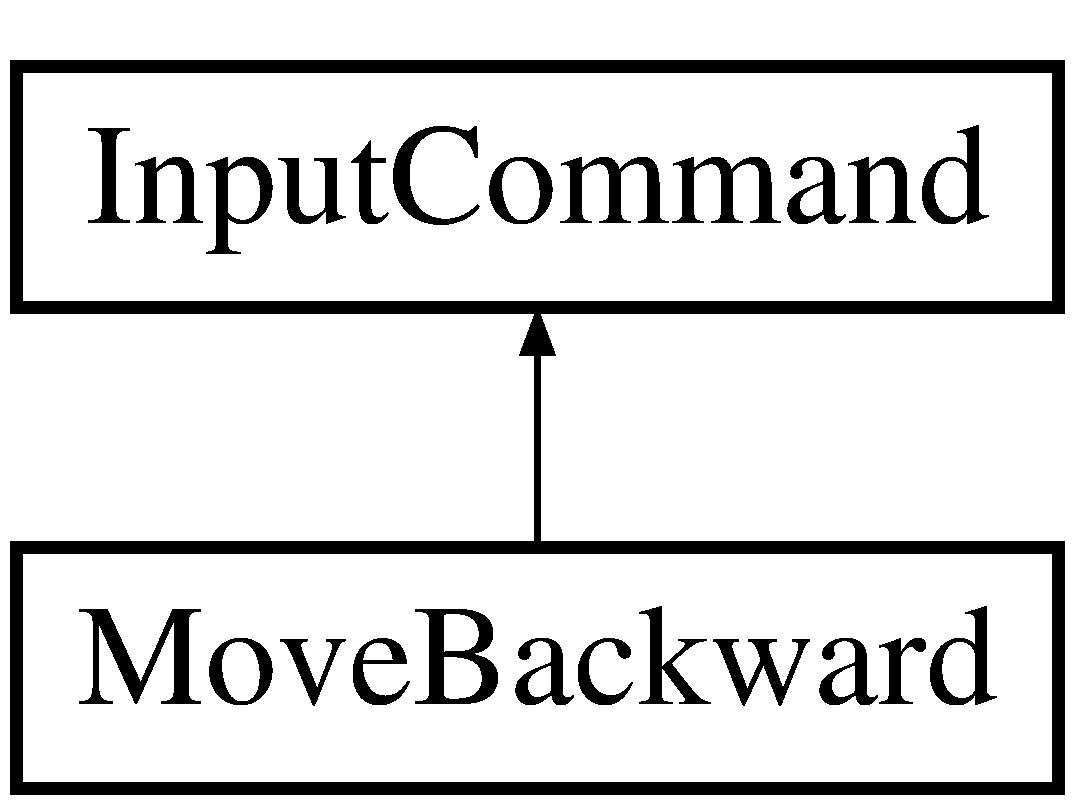
\includegraphics[height=2.000000cm]{class_move_backward}
\end{center}
\end{figure}
\subsection*{Additional Inherited Members}


The documentation for this class was generated from the following file\+:\begin{DoxyCompactItemize}
\item 
Game\+Engine/include/\mbox{\hyperlink{_input_handler_8h}{Input\+Handler.\+h}}\end{DoxyCompactItemize}

\hypertarget{class_move_component}{}\section{Move\+Component Class Reference}
\label{class_move_component}\index{Move\+Component@{Move\+Component}}


{\ttfamily \#include $<$Move\+Component.\+h$>$}

Inheritance diagram for Move\+Component\+:\begin{figure}[H]
\begin{center}
\leavevmode
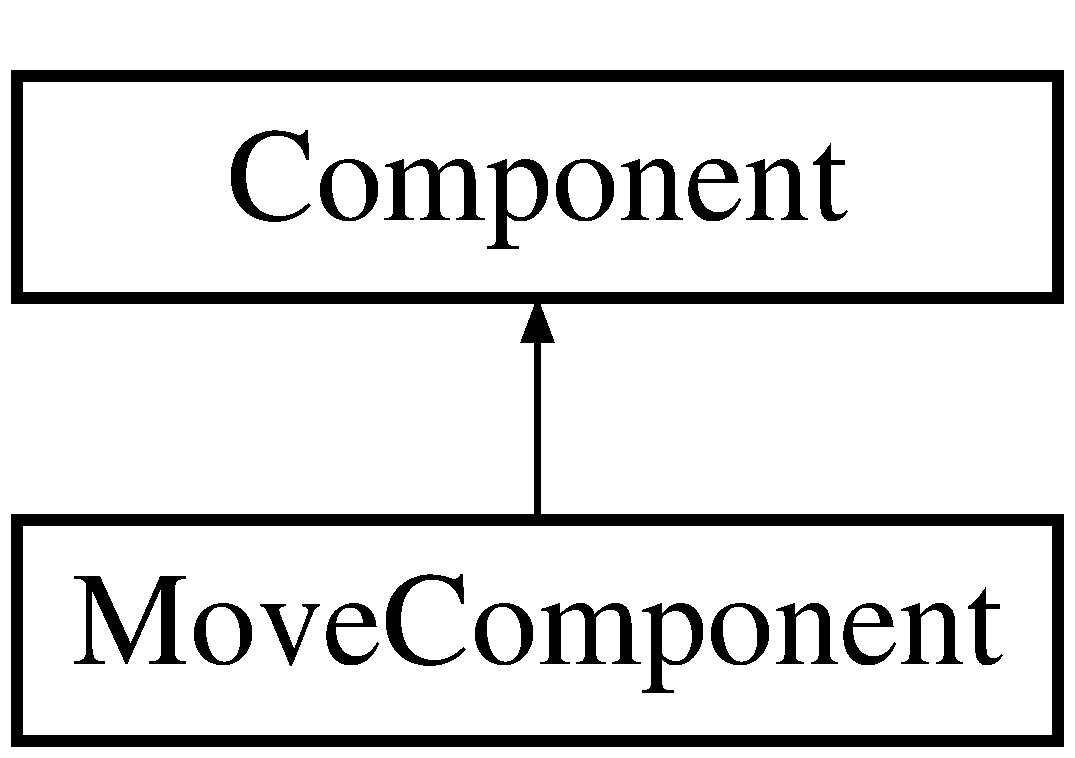
\includegraphics[height=2.000000cm]{class_move_component}
\end{center}
\end{figure}
\subsection*{Public Member Functions}
\begin{DoxyCompactItemize}
\item 
\mbox{\hyperlink{class_move_component_aee1693ed79d7d930e87ef35e40bbfcfa}{Move\+Component}} (\mbox{\hyperlink{class_game_object}{Game\+Object}} $\ast$movable\+Object)
\item 
\mbox{\hyperlink{class_move_component_a5e8430c851f1d83f2b8222c3c4ec097d}{$\sim$\+Move\+Component}} ()
\item 
void \mbox{\hyperlink{class_move_component_aac8549ecd0670b2b8830d43019d58ea4}{On\+Update}} (float dt) override
\item 
void \mbox{\hyperlink{class_move_component_a27146b88beda6223ed9f4a82c47a917a}{On\+Message}} (const std\+::string m) override
\end{DoxyCompactItemize}


\subsection{Constructor \& Destructor Documentation}
\mbox{\Hypertarget{class_move_component_aee1693ed79d7d930e87ef35e40bbfcfa}\label{class_move_component_aee1693ed79d7d930e87ef35e40bbfcfa}} 
\index{Move\+Component@{Move\+Component}!Move\+Component@{Move\+Component}}
\index{Move\+Component@{Move\+Component}!Move\+Component@{Move\+Component}}
\subsubsection{\texorpdfstring{Move\+Component()}{MoveComponent()}}
{\footnotesize\ttfamily Move\+Component\+::\+Move\+Component (\begin{DoxyParamCaption}\item[{\mbox{\hyperlink{class_game_object}{Game\+Object}} $\ast$}]{movable\+Object }\end{DoxyParamCaption})\hspace{0.3cm}{\ttfamily [inline]}}

Constructor Param One \+: \mbox{\hyperlink{class_this}{This}} is the object this component is connected to. \mbox{\Hypertarget{class_move_component_a5e8430c851f1d83f2b8222c3c4ec097d}\label{class_move_component_a5e8430c851f1d83f2b8222c3c4ec097d}} 
\index{Move\+Component@{Move\+Component}!````~Move\+Component@{$\sim$\+Move\+Component}}
\index{````~Move\+Component@{$\sim$\+Move\+Component}!Move\+Component@{Move\+Component}}
\subsubsection{\texorpdfstring{$\sim$\+Move\+Component()}{~MoveComponent()}}
{\footnotesize\ttfamily Move\+Component\+::$\sim$\+Move\+Component (\begin{DoxyParamCaption}{ }\end{DoxyParamCaption})\hspace{0.3cm}{\ttfamily [inline]}}

Deconstructor 

\subsection{Member Function Documentation}
\mbox{\Hypertarget{class_move_component_a27146b88beda6223ed9f4a82c47a917a}\label{class_move_component_a27146b88beda6223ed9f4a82c47a917a}} 
\index{Move\+Component@{Move\+Component}!On\+Message@{On\+Message}}
\index{On\+Message@{On\+Message}!Move\+Component@{Move\+Component}}
\subsubsection{\texorpdfstring{On\+Message()}{OnMessage()}}
{\footnotesize\ttfamily void Move\+Component\+::\+On\+Message (\begin{DoxyParamCaption}\item[{const std\+::string}]{m }\end{DoxyParamCaption})\hspace{0.3cm}{\ttfamily [inline]}, {\ttfamily [override]}, {\ttfamily [virtual]}}

On\+Message \+: \mbox{\hyperlink{class_this}{This}} will be use to react to a key press if required. 

Implements \mbox{\hyperlink{class_component_a1a880fe5e212cd7ef8241e220660417d}{Component}}.

\mbox{\Hypertarget{class_move_component_aac8549ecd0670b2b8830d43019d58ea4}\label{class_move_component_aac8549ecd0670b2b8830d43019d58ea4}} 
\index{Move\+Component@{Move\+Component}!On\+Update@{On\+Update}}
\index{On\+Update@{On\+Update}!Move\+Component@{Move\+Component}}
\subsubsection{\texorpdfstring{On\+Update()}{OnUpdate()}}
{\footnotesize\ttfamily void Move\+Component\+::\+On\+Update (\begin{DoxyParamCaption}\item[{float}]{dt }\end{DoxyParamCaption})\hspace{0.3cm}{\ttfamily [inline]}, {\ttfamily [override]}, {\ttfamily [virtual]}}

On\+Update \+: \mbox{\hyperlink{class_this}{This}} will be used to call any update functions for this component. 

Implements \mbox{\hyperlink{class_component_ab71d7f4b6d8792287a9b0c9e045acbe0}{Component}}.



The documentation for this class was generated from the following file\+:\begin{DoxyCompactItemize}
\item 
Game\+Engine/include/\mbox{\hyperlink{_move_component_8h}{Move\+Component.\+h}}\end{DoxyCompactItemize}

\hypertarget{class_move_forward}{}\section{Move\+Forward Class Reference}
\label{class_move_forward}\index{Move\+Forward@{Move\+Forward}}


{\ttfamily \#include $<$Input\+Handler.\+h$>$}

Inheritance diagram for Move\+Forward\+:\begin{figure}[H]
\begin{center}
\leavevmode
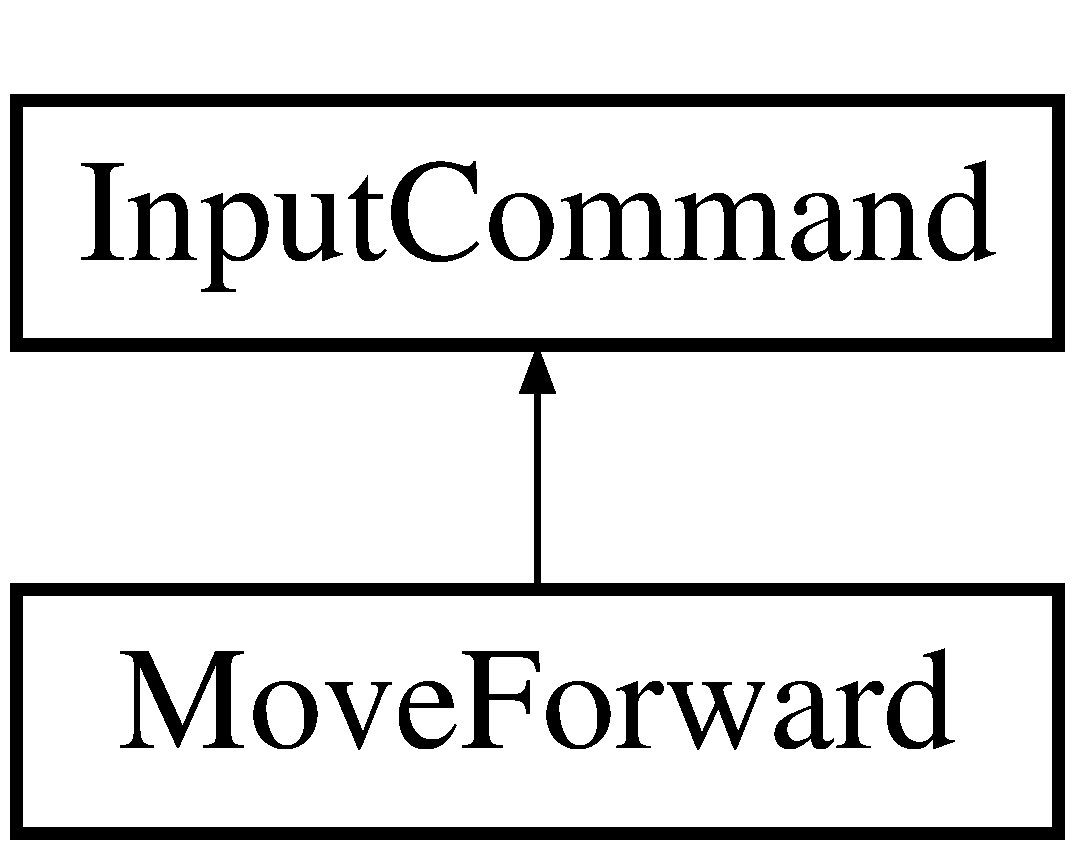
\includegraphics[height=2.000000cm]{class_move_forward}
\end{center}
\end{figure}
\subsection*{Additional Inherited Members}


The documentation for this class was generated from the following file\+:\begin{DoxyCompactItemize}
\item 
Game\+Engine/include/\mbox{\hyperlink{_input_handler_8h}{Input\+Handler.\+h}}\end{DoxyCompactItemize}

\hypertarget{class_move_left}{}\section{Move\+Left Class Reference}
\label{class_move_left}\index{Move\+Left@{Move\+Left}}


{\ttfamily \#include $<$Input\+Handler.\+h$>$}

Inheritance diagram for Move\+Left\+:\begin{figure}[H]
\begin{center}
\leavevmode
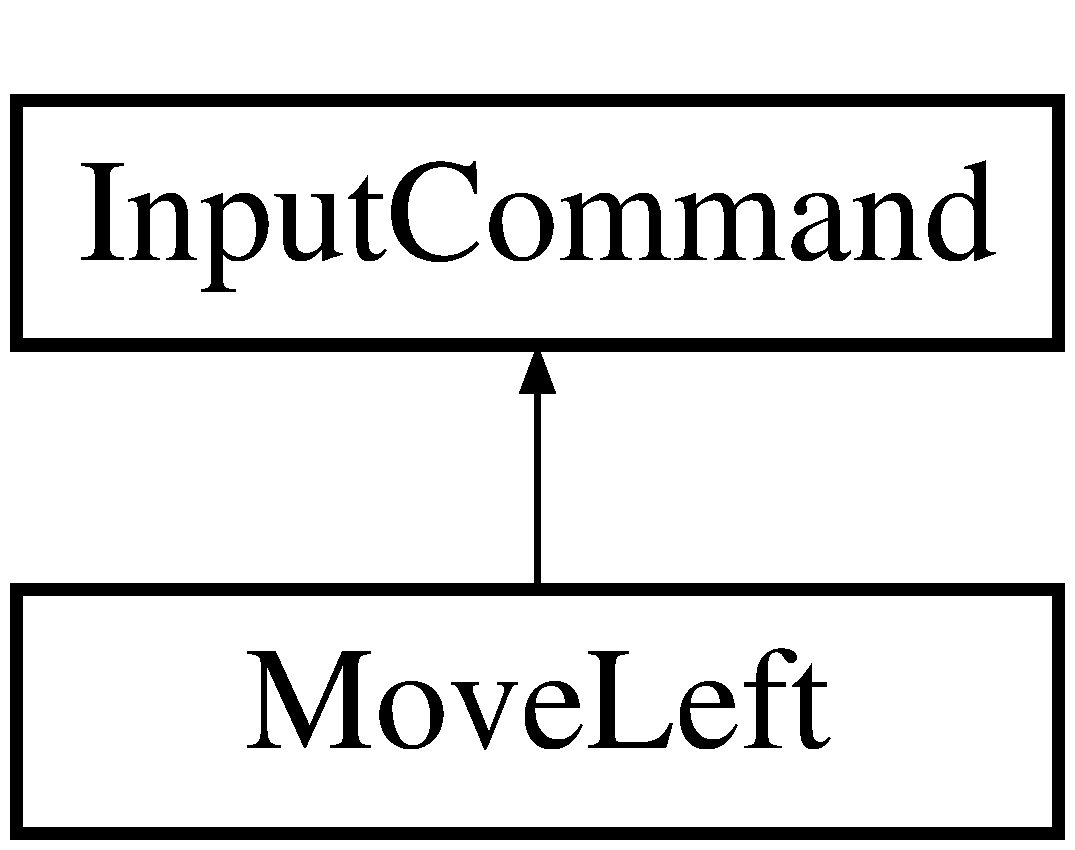
\includegraphics[height=2.000000cm]{class_move_left}
\end{center}
\end{figure}
\subsection*{Additional Inherited Members}


The documentation for this class was generated from the following file\+:\begin{DoxyCompactItemize}
\item 
Game\+Engine/include/\mbox{\hyperlink{_input_handler_8h}{Input\+Handler.\+h}}\end{DoxyCompactItemize}

\hypertarget{class_move_right}{}\section{Move\+Right Class Reference}
\label{class_move_right}\index{Move\+Right@{Move\+Right}}


{\ttfamily \#include $<$Input\+Handler.\+h$>$}

Inheritance diagram for Move\+Right\+:\begin{figure}[H]
\begin{center}
\leavevmode
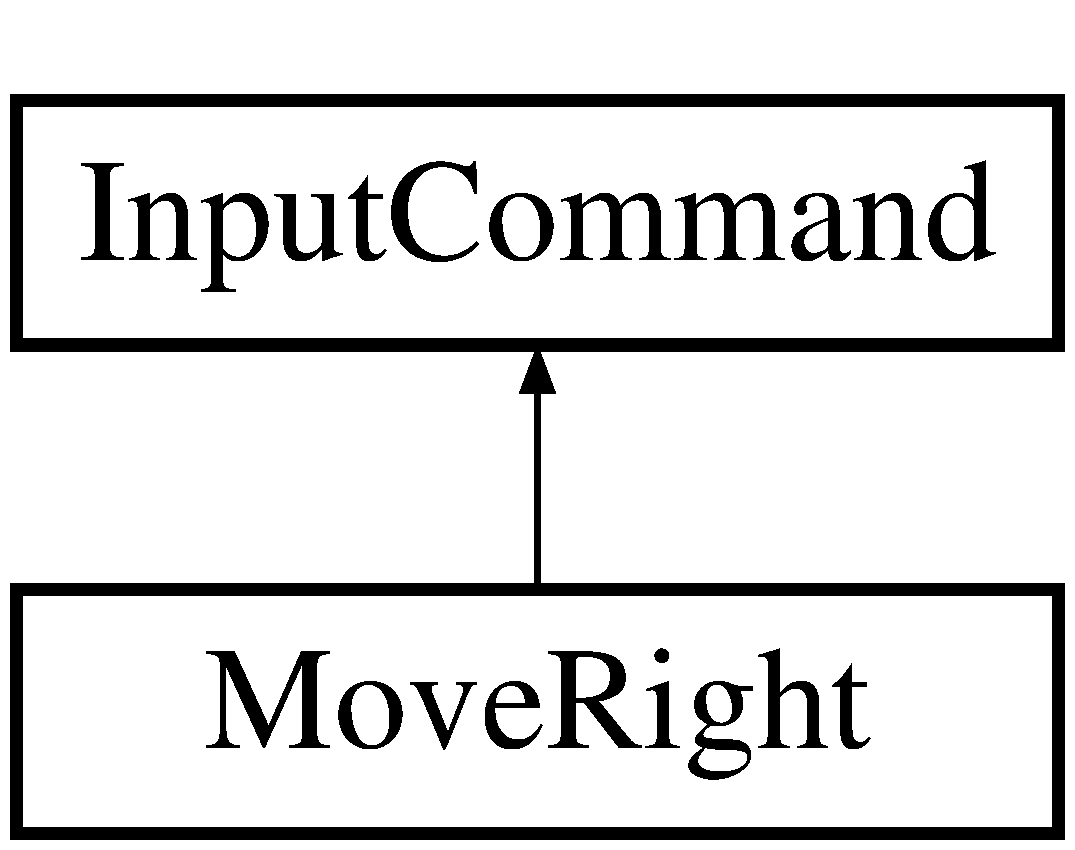
\includegraphics[height=2.000000cm]{class_move_right}
\end{center}
\end{figure}
\subsection*{Additional Inherited Members}


The documentation for this class was generated from the following file\+:\begin{DoxyCompactItemize}
\item 
Game\+Engine/include/\mbox{\hyperlink{_input_handler_8h}{Input\+Handler.\+h}}\end{DoxyCompactItemize}

\hypertarget{class_next_camera}{}\section{Next\+Camera Class Reference}
\label{class_next_camera}\index{Next\+Camera@{Next\+Camera}}


{\ttfamily \#include $<$Input\+Handler.\+h$>$}

Inheritance diagram for Next\+Camera\+:\begin{figure}[H]
\begin{center}
\leavevmode
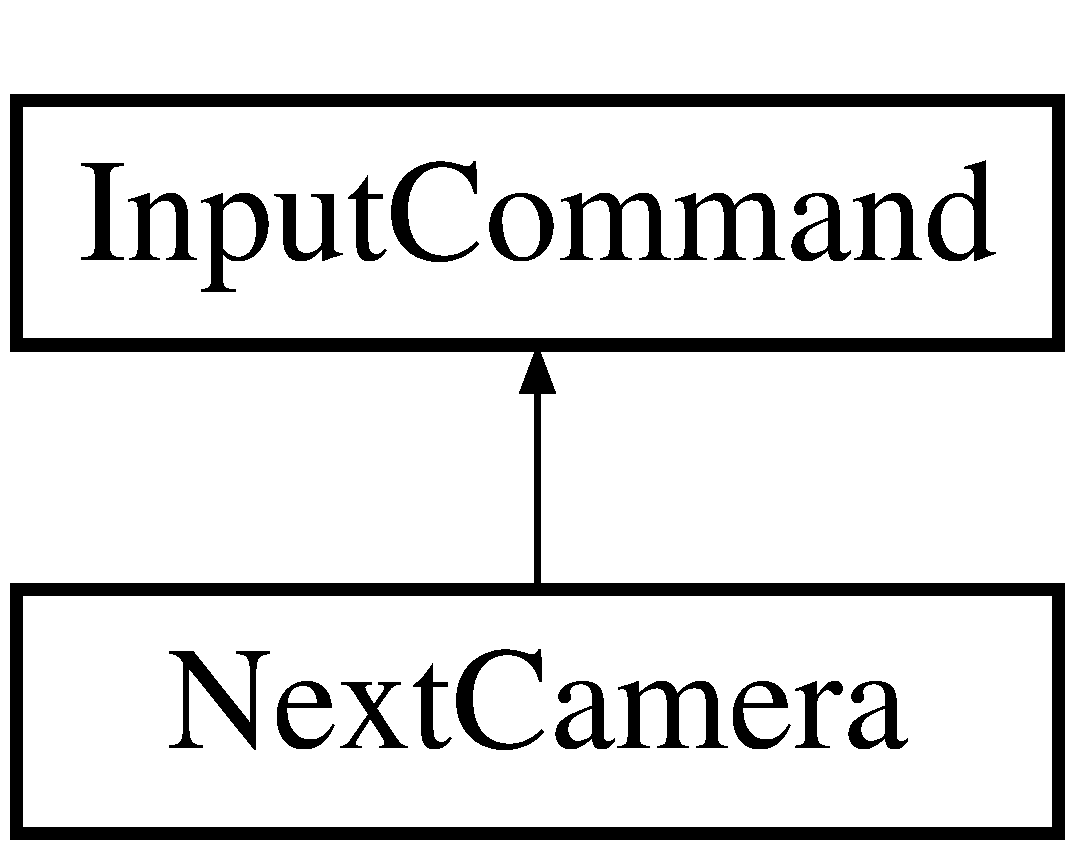
\includegraphics[height=2.000000cm]{class_next_camera}
\end{center}
\end{figure}
\subsection*{Additional Inherited Members}


The documentation for this class was generated from the following file\+:\begin{DoxyCompactItemize}
\item 
Game\+Engine/include/\mbox{\hyperlink{_input_handler_8h}{Input\+Handler.\+h}}\end{DoxyCompactItemize}

\hypertarget{class_red_component}{}\section{Red\+Component Class Reference}
\label{class_red_component}\index{Red\+Component@{Red\+Component}}


{\ttfamily \#include $<$Colour\+Component.\+h$>$}

Inheritance diagram for Red\+Component\+:\begin{figure}[H]
\begin{center}
\leavevmode
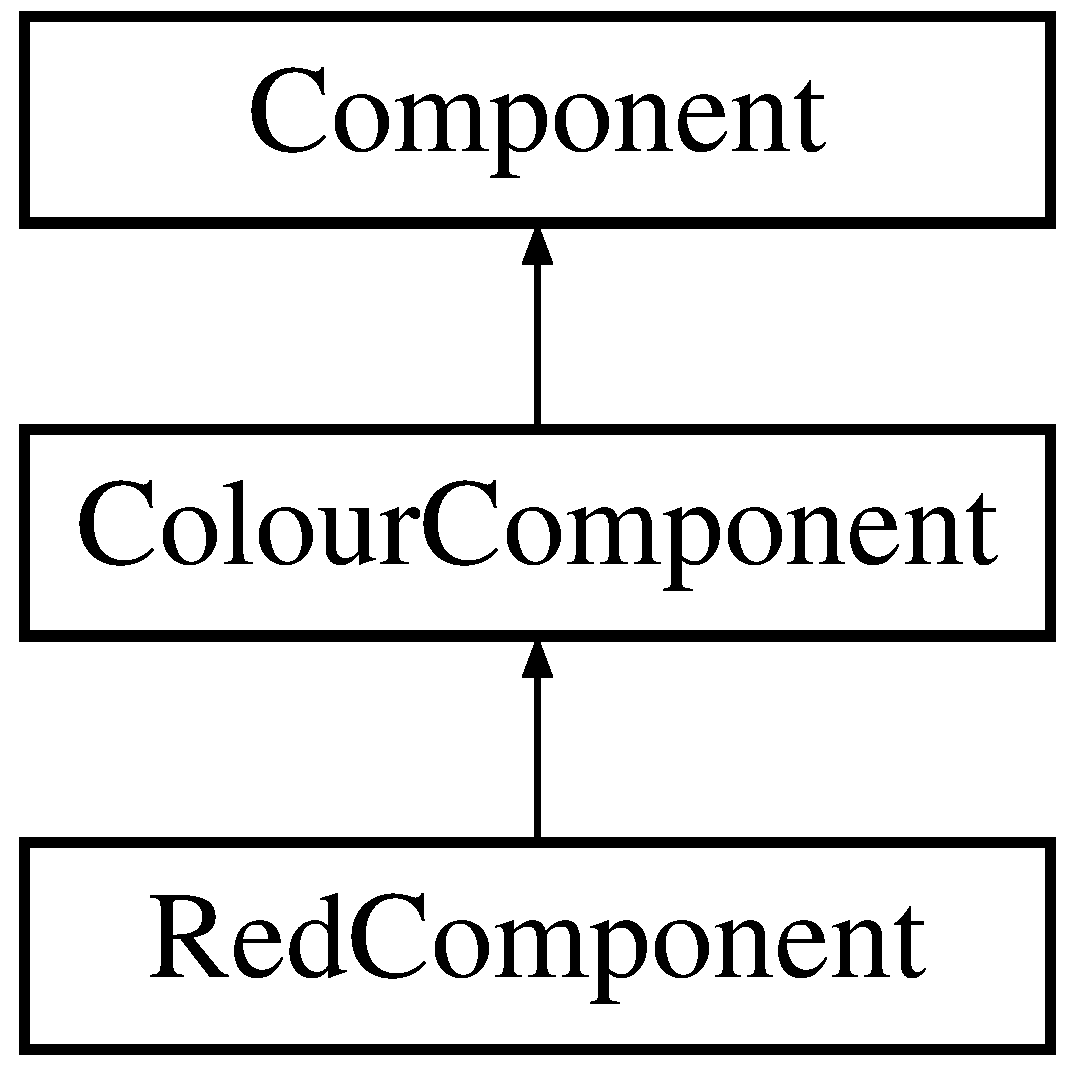
\includegraphics[height=3.000000cm]{class_red_component}
\end{center}
\end{figure}
\subsection*{Additional Inherited Members}


The documentation for this class was generated from the following file\+:\begin{DoxyCompactItemize}
\item 
Game\+Engine/include/\mbox{\hyperlink{_colour_component_8h}{Colour\+Component.\+h}}\end{DoxyCompactItemize}

\hypertarget{class_renderer}{}\section{Renderer Class Reference}
\label{class_renderer}\index{Renderer@{Renderer}}


{\ttfamily \#include $<$Renderer.\+h$>$}

\subsection*{Public Member Functions}
\begin{DoxyCompactItemize}
\item 
\mbox{\hyperlink{class_renderer_a7ebf46f54dab9905f79b80f7fddb76a6}{Renderer}} ()
\item 
\mbox{\hyperlink{class_renderer_afeee408862d5bd6255a6882d47e6d5cd}{$\sim$\+Renderer}} ()
\item 
void \mbox{\hyperlink{class_renderer_a5413bf99fb5a945ca2be17b83cbd43e5}{m\+\_\+\+Render}} (\mbox{\hyperlink{class_game_object}{Game\+Object}} $\ast$drawable, \mbox{\hyperlink{class_i_engine_core}{I\+Engine\+Core}} $\ast$core)
\item 
void \mbox{\hyperlink{class_renderer_a6852a562bd5a7ed130c16bb1d1eaebdc}{m\+\_\+\+Render}} (std\+::vector$<$ \mbox{\hyperlink{class_game_object}{Game\+Object}} $>$ \&drawable, \mbox{\hyperlink{class_i_engine_core}{I\+Engine\+Core}} $\ast$core)
\item 
void \mbox{\hyperlink{class_renderer_a2f7d175aafc8170e9082ea39abae1628}{m\+\_\+\+Render}} (std\+::vector$<$ \mbox{\hyperlink{class_game_object}{Game\+Object}} $\ast$$>$ drawable, \mbox{\hyperlink{class_i_engine_core}{I\+Engine\+Core}} $\ast$core)
\end{DoxyCompactItemize}


\subsection{Constructor \& Destructor Documentation}
\mbox{\Hypertarget{class_renderer_a7ebf46f54dab9905f79b80f7fddb76a6}\label{class_renderer_a7ebf46f54dab9905f79b80f7fddb76a6}} 
\index{Renderer@{Renderer}!Renderer@{Renderer}}
\index{Renderer@{Renderer}!Renderer@{Renderer}}
\subsubsection{\texorpdfstring{Renderer()}{Renderer()}}
{\footnotesize\ttfamily Renderer\+::\+Renderer (\begin{DoxyParamCaption}{ }\end{DoxyParamCaption})}

Constructor \mbox{\Hypertarget{class_renderer_afeee408862d5bd6255a6882d47e6d5cd}\label{class_renderer_afeee408862d5bd6255a6882d47e6d5cd}} 
\index{Renderer@{Renderer}!````~Renderer@{$\sim$\+Renderer}}
\index{````~Renderer@{$\sim$\+Renderer}!Renderer@{Renderer}}
\subsubsection{\texorpdfstring{$\sim$\+Renderer()}{~Renderer()}}
{\footnotesize\ttfamily Renderer\+::$\sim$\+Renderer (\begin{DoxyParamCaption}{ }\end{DoxyParamCaption})}

Deconstructor 

\subsection{Member Function Documentation}
\mbox{\Hypertarget{class_renderer_a5413bf99fb5a945ca2be17b83cbd43e5}\label{class_renderer_a5413bf99fb5a945ca2be17b83cbd43e5}} 
\index{Renderer@{Renderer}!m\+\_\+\+Render@{m\+\_\+\+Render}}
\index{m\+\_\+\+Render@{m\+\_\+\+Render}!Renderer@{Renderer}}
\subsubsection{\texorpdfstring{m\+\_\+\+Render()}{m\_Render()}\hspace{0.1cm}{\footnotesize\ttfamily [1/3]}}
{\footnotesize\ttfamily void Renderer\+::m\+\_\+\+Render (\begin{DoxyParamCaption}\item[{\mbox{\hyperlink{class_game_object}{Game\+Object}} $\ast$}]{drawable,  }\item[{\mbox{\hyperlink{class_i_engine_core}{I\+Engine\+Core}} $\ast$}]{core }\end{DoxyParamCaption})}

Render \+: \mbox{\hyperlink{class_this}{This}} will render the game object passed into it. Param One \+: \mbox{\hyperlink{class_the}{The}} game object to draw. Param Two \+: \mbox{\hyperlink{class_the}{The}} current engine core for the game. \mbox{\Hypertarget{class_renderer_a6852a562bd5a7ed130c16bb1d1eaebdc}\label{class_renderer_a6852a562bd5a7ed130c16bb1d1eaebdc}} 
\index{Renderer@{Renderer}!m\+\_\+\+Render@{m\+\_\+\+Render}}
\index{m\+\_\+\+Render@{m\+\_\+\+Render}!Renderer@{Renderer}}
\subsubsection{\texorpdfstring{m\+\_\+\+Render()}{m\_Render()}\hspace{0.1cm}{\footnotesize\ttfamily [2/3]}}
{\footnotesize\ttfamily void Renderer\+::m\+\_\+\+Render (\begin{DoxyParamCaption}\item[{std\+::vector$<$ \mbox{\hyperlink{class_game_object}{Game\+Object}} $>$ \&}]{drawable,  }\item[{\mbox{\hyperlink{class_i_engine_core}{I\+Engine\+Core}} $\ast$}]{core }\end{DoxyParamCaption})}

Render \+: \mbox{\hyperlink{class_this}{This}} will render the game object passed into it. Param One \+: A list of game objects to render. Param Two \+: \mbox{\hyperlink{class_the}{The}} current engine core for the game. \mbox{\Hypertarget{class_renderer_a2f7d175aafc8170e9082ea39abae1628}\label{class_renderer_a2f7d175aafc8170e9082ea39abae1628}} 
\index{Renderer@{Renderer}!m\+\_\+\+Render@{m\+\_\+\+Render}}
\index{m\+\_\+\+Render@{m\+\_\+\+Render}!Renderer@{Renderer}}
\subsubsection{\texorpdfstring{m\+\_\+\+Render()}{m\_Render()}\hspace{0.1cm}{\footnotesize\ttfamily [3/3]}}
{\footnotesize\ttfamily void Renderer\+::m\+\_\+\+Render (\begin{DoxyParamCaption}\item[{std\+::vector$<$ \mbox{\hyperlink{class_game_object}{Game\+Object}} $\ast$$>$}]{drawable,  }\item[{\mbox{\hyperlink{class_i_engine_core}{I\+Engine\+Core}} $\ast$}]{core }\end{DoxyParamCaption})}

Render \+: \mbox{\hyperlink{class_this}{This}} will render the game object passed into it. Param One \+: A list of game objects to render. Param Two \+: \mbox{\hyperlink{class_the}{The}} current engine core for the game. 

The documentation for this class was generated from the following file\+:\begin{DoxyCompactItemize}
\item 
Game\+Engine/include/\mbox{\hyperlink{_renderer_8h}{Renderer.\+h}}\end{DoxyCompactItemize}

\hypertarget{class_rot_left}{}\section{Rot\+Left Class Reference}
\label{class_rot_left}\index{Rot\+Left@{Rot\+Left}}


{\ttfamily \#include $<$Input\+Handler.\+h$>$}

Inheritance diagram for Rot\+Left\+:\begin{figure}[H]
\begin{center}
\leavevmode
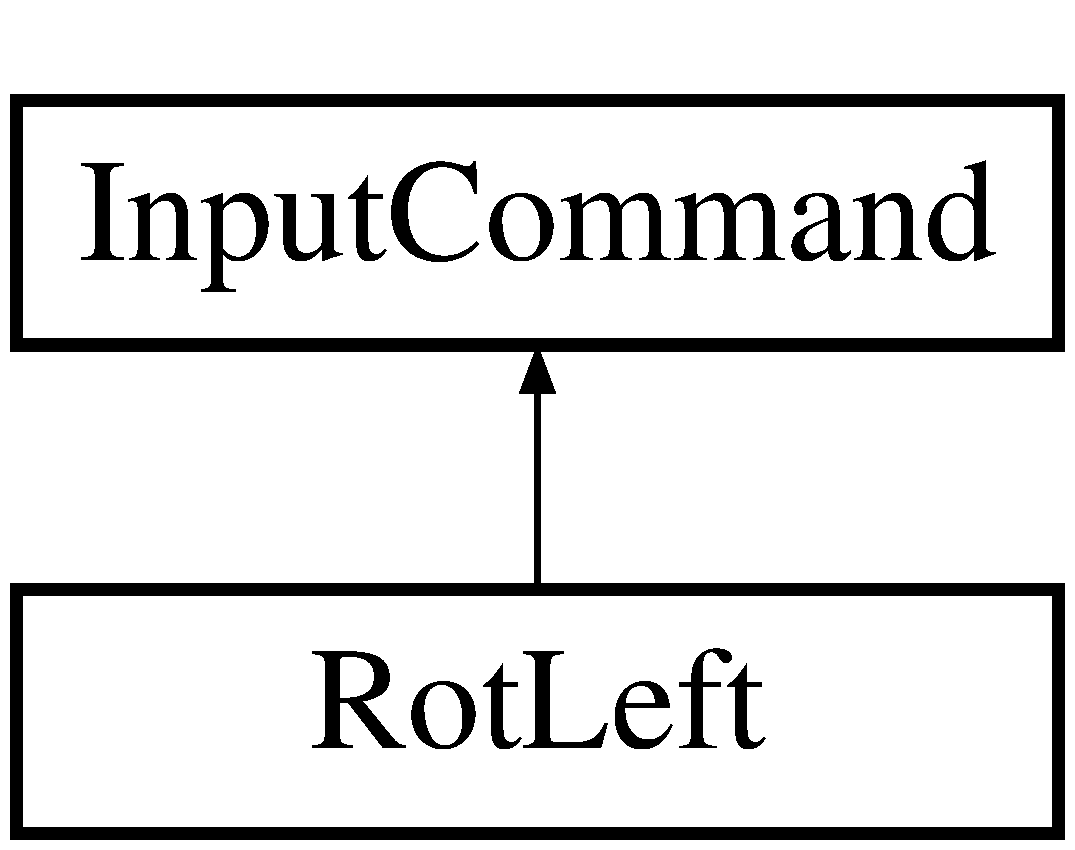
\includegraphics[height=2.000000cm]{class_rot_left}
\end{center}
\end{figure}
\subsection*{Additional Inherited Members}


The documentation for this class was generated from the following file\+:\begin{DoxyCompactItemize}
\item 
Game\+Engine/include/\mbox{\hyperlink{_input_handler_8h}{Input\+Handler.\+h}}\end{DoxyCompactItemize}

\hypertarget{class_rot_right}{}\section{Rot\+Right Class Reference}
\label{class_rot_right}\index{Rot\+Right@{Rot\+Right}}


{\ttfamily \#include $<$Input\+Handler.\+h$>$}

Inheritance diagram for Rot\+Right\+:\begin{figure}[H]
\begin{center}
\leavevmode
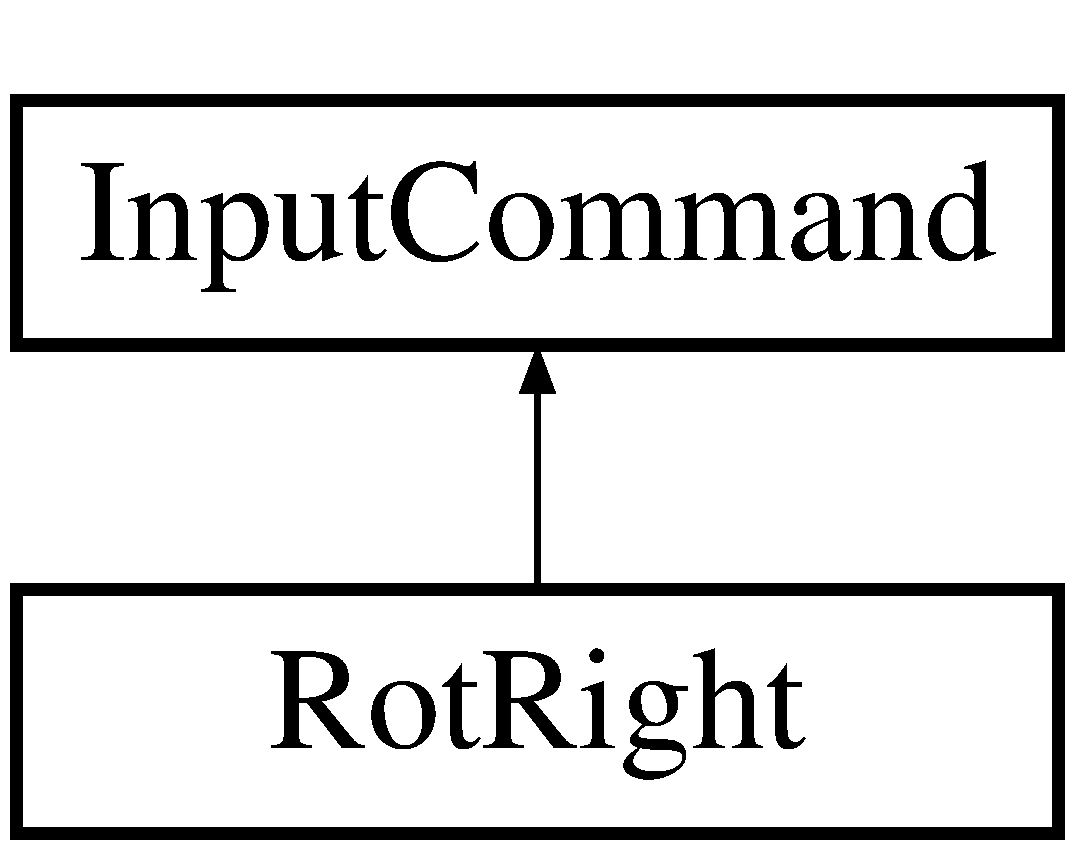
\includegraphics[height=2.000000cm]{class_rot_right}
\end{center}
\end{figure}
\subsection*{Additional Inherited Members}


The documentation for this class was generated from the following file\+:\begin{DoxyCompactItemize}
\item 
Game\+Engine/include/\mbox{\hyperlink{_input_handler_8h}{Input\+Handler.\+h}}\end{DoxyCompactItemize}

\hypertarget{class_scene}{}\section{Scene Class Reference}
\label{class_scene}\index{Scene@{Scene}}


{\ttfamily \#include $<$Scene.\+h$>$}

\subsection*{Public Member Functions}
\begin{DoxyCompactItemize}
\item 
\mbox{\hyperlink{class_scene_a2d8d697e4b432199f7c663e51ea1a62d}{Scene}} (std\+::string level\+File)
\item 
\mbox{\hyperlink{class_scene_a3b8cec2e32546713915f8c6303c951f1}{$\sim$\+Scene}} ()
\item 
void \mbox{\hyperlink{class_scene_a2d84a7dbabaf8b0dd135d754200cb126}{m\+\_\+\+Update}} ()
\item 
void \mbox{\hyperlink{class_scene_a09f503e90af9f19de0f461b827425ccb}{m\+\_\+\+Render}} (\mbox{\hyperlink{class_i_engine_core}{I\+Engine\+Core}} $\ast$engine\+Interface)
\item 
std\+::vector$<$ \mbox{\hyperlink{class_game_object}{Game\+Object}} $>$ \mbox{\hyperlink{class_scene_a183135dcbd5fa1c27da8246d9a185397}{m\+\_\+\+Get\+Game\+Objects}} ()
\item 
bool \mbox{\hyperlink{class_scene_ab44df8bc0f251a99a35b1c876cb02b46}{m\+\_\+\+Load\+Level\+Json}} (std\+::string level\+File)
\end{DoxyCompactItemize}


\subsection{Constructor \& Destructor Documentation}
\mbox{\Hypertarget{class_scene_a2d8d697e4b432199f7c663e51ea1a62d}\label{class_scene_a2d8d697e4b432199f7c663e51ea1a62d}} 
\index{Scene@{Scene}!Scene@{Scene}}
\index{Scene@{Scene}!Scene@{Scene}}
\subsubsection{\texorpdfstring{Scene()}{Scene()}}
{\footnotesize\ttfamily Scene\+::\+Scene (\begin{DoxyParamCaption}\item[{std\+::string}]{level\+File }\end{DoxyParamCaption})}

Constructor Param One \+: \mbox{\hyperlink{class_the}{The}} location for the level, to load. \mbox{\Hypertarget{class_scene_a3b8cec2e32546713915f8c6303c951f1}\label{class_scene_a3b8cec2e32546713915f8c6303c951f1}} 
\index{Scene@{Scene}!````~Scene@{$\sim$\+Scene}}
\index{````~Scene@{$\sim$\+Scene}!Scene@{Scene}}
\subsubsection{\texorpdfstring{$\sim$\+Scene()}{~Scene()}}
{\footnotesize\ttfamily Scene\+::$\sim$\+Scene (\begin{DoxyParamCaption}{ }\end{DoxyParamCaption})}

Deconstructor 

\subsection{Member Function Documentation}
\mbox{\Hypertarget{class_scene_a183135dcbd5fa1c27da8246d9a185397}\label{class_scene_a183135dcbd5fa1c27da8246d9a185397}} 
\index{Scene@{Scene}!m\+\_\+\+Get\+Game\+Objects@{m\+\_\+\+Get\+Game\+Objects}}
\index{m\+\_\+\+Get\+Game\+Objects@{m\+\_\+\+Get\+Game\+Objects}!Scene@{Scene}}
\subsubsection{\texorpdfstring{m\+\_\+\+Get\+Game\+Objects()}{m\_GetGameObjects()}}
{\footnotesize\ttfamily std\+::vector$<$\mbox{\hyperlink{class_game_object}{Game\+Object}}$>$ Scene\+::m\+\_\+\+Get\+Game\+Objects (\begin{DoxyParamCaption}{ }\end{DoxyParamCaption})}

Get\+Game\+Objects \+: \mbox{\hyperlink{class_used}{Used}} to get the list of game object currently in the scene. \mbox{\Hypertarget{class_scene_ab44df8bc0f251a99a35b1c876cb02b46}\label{class_scene_ab44df8bc0f251a99a35b1c876cb02b46}} 
\index{Scene@{Scene}!m\+\_\+\+Load\+Level\+Json@{m\+\_\+\+Load\+Level\+Json}}
\index{m\+\_\+\+Load\+Level\+Json@{m\+\_\+\+Load\+Level\+Json}!Scene@{Scene}}
\subsubsection{\texorpdfstring{m\+\_\+\+Load\+Level\+Json()}{m\_LoadLevelJson()}}
{\footnotesize\ttfamily bool Scene\+::m\+\_\+\+Load\+Level\+Json (\begin{DoxyParamCaption}\item[{std\+::string}]{level\+File }\end{DoxyParamCaption})}

Load\+Level\+Json \+: \mbox{\hyperlink{class_this}{This}} will load the game scene from a json file. \mbox{\Hypertarget{class_scene_a09f503e90af9f19de0f461b827425ccb}\label{class_scene_a09f503e90af9f19de0f461b827425ccb}} 
\index{Scene@{Scene}!m\+\_\+\+Render@{m\+\_\+\+Render}}
\index{m\+\_\+\+Render@{m\+\_\+\+Render}!Scene@{Scene}}
\subsubsection{\texorpdfstring{m\+\_\+\+Render()}{m\_Render()}}
{\footnotesize\ttfamily void Scene\+::m\+\_\+\+Render (\begin{DoxyParamCaption}\item[{\mbox{\hyperlink{class_i_engine_core}{I\+Engine\+Core}} $\ast$}]{engine\+Interface }\end{DoxyParamCaption})}

Render \+: \mbox{\hyperlink{class_used}{Used}} to render the current scene. Param One \+: \mbox{\hyperlink{class_the}{The}} current engine core being used. \mbox{\Hypertarget{class_scene_a2d84a7dbabaf8b0dd135d754200cb126}\label{class_scene_a2d84a7dbabaf8b0dd135d754200cb126}} 
\index{Scene@{Scene}!m\+\_\+\+Update@{m\+\_\+\+Update}}
\index{m\+\_\+\+Update@{m\+\_\+\+Update}!Scene@{Scene}}
\subsubsection{\texorpdfstring{m\+\_\+\+Update()}{m\_Update()}}
{\footnotesize\ttfamily void Scene\+::m\+\_\+\+Update (\begin{DoxyParamCaption}{ }\end{DoxyParamCaption})}

Update \+: \mbox{\hyperlink{class_used}{Used}} to update the current scene. 

The documentation for this class was generated from the following file\+:\begin{DoxyCompactItemize}
\item 
Game\+Engine/include/\mbox{\hyperlink{_scene_8h}{Scene.\+h}}\end{DoxyCompactItemize}

\hypertarget{structstbi__io__callbacks}{}\section{stbi\+\_\+io\+\_\+callbacks Struct Reference}
\label{structstbi__io__callbacks}\index{stbi\+\_\+io\+\_\+callbacks@{stbi\+\_\+io\+\_\+callbacks}}


{\ttfamily \#include $<$stb\+\_\+image.\+h$>$}

\subsection*{Public Attributes}
\begin{DoxyCompactItemize}
\item 
int($\ast$ \mbox{\hyperlink{structstbi__io__callbacks_a623e46b3a2a019611601409926283a88}{read}} )(void $\ast$user, char $\ast$data, int size)
\item 
void($\ast$ \mbox{\hyperlink{structstbi__io__callbacks_a257aac5480a90a6c4b8fbe86c1b01068}{skip}} )(void $\ast$user, int n)
\item 
int($\ast$ \mbox{\hyperlink{structstbi__io__callbacks_a319639db2f76e715eed7a7a974136832}{eof}} )(void $\ast$user)
\end{DoxyCompactItemize}


\subsection{Member Data Documentation}
\mbox{\Hypertarget{structstbi__io__callbacks_a319639db2f76e715eed7a7a974136832}\label{structstbi__io__callbacks_a319639db2f76e715eed7a7a974136832}} 
\index{stbi\+\_\+io\+\_\+callbacks@{stbi\+\_\+io\+\_\+callbacks}!eof@{eof}}
\index{eof@{eof}!stbi\+\_\+io\+\_\+callbacks@{stbi\+\_\+io\+\_\+callbacks}}
\subsubsection{\texorpdfstring{eof}{eof}}
{\footnotesize\ttfamily int($\ast$ stbi\+\_\+io\+\_\+callbacks\+::eof) (void $\ast$user)}

\mbox{\Hypertarget{structstbi__io__callbacks_a623e46b3a2a019611601409926283a88}\label{structstbi__io__callbacks_a623e46b3a2a019611601409926283a88}} 
\index{stbi\+\_\+io\+\_\+callbacks@{stbi\+\_\+io\+\_\+callbacks}!read@{read}}
\index{read@{read}!stbi\+\_\+io\+\_\+callbacks@{stbi\+\_\+io\+\_\+callbacks}}
\subsubsection{\texorpdfstring{read}{read}}
{\footnotesize\ttfamily int($\ast$ stbi\+\_\+io\+\_\+callbacks\+::read) (void $\ast$user, char $\ast$data, int size)}

\mbox{\Hypertarget{structstbi__io__callbacks_a257aac5480a90a6c4b8fbe86c1b01068}\label{structstbi__io__callbacks_a257aac5480a90a6c4b8fbe86c1b01068}} 
\index{stbi\+\_\+io\+\_\+callbacks@{stbi\+\_\+io\+\_\+callbacks}!skip@{skip}}
\index{skip@{skip}!stbi\+\_\+io\+\_\+callbacks@{stbi\+\_\+io\+\_\+callbacks}}
\subsubsection{\texorpdfstring{skip}{skip}}
{\footnotesize\ttfamily void($\ast$ stbi\+\_\+io\+\_\+callbacks\+::skip) (void $\ast$user, int n)}



The documentation for this struct was generated from the following file\+:\begin{DoxyCompactItemize}
\item 
Game\+Engine/include/\mbox{\hyperlink{stb__image_8h}{stb\+\_\+image.\+h}}\end{DoxyCompactItemize}

\hypertarget{struct_texture}{}\section{Texture Struct Reference}
\label{struct_texture}\index{Texture@{Texture}}


{\ttfamily \#include $<$Mesh.\+h$>$}

\subsection*{Public Attributes}
\begin{DoxyCompactItemize}
\item 
unsigned int \mbox{\hyperlink{struct_texture_aed42161a5c00b6020c85833401da6da6}{id}}
\item 
string \mbox{\hyperlink{struct_texture_adacb495ed5140ec76a09cd130e7d5c32}{type}}
\item 
ai\+String \mbox{\hyperlink{struct_texture_a69c8def64c608063b2ecb7fd785121ee}{filepath}}
\end{DoxyCompactItemize}


\subsection{Member Data Documentation}
\mbox{\Hypertarget{struct_texture_a69c8def64c608063b2ecb7fd785121ee}\label{struct_texture_a69c8def64c608063b2ecb7fd785121ee}} 
\index{Texture@{Texture}!filepath@{filepath}}
\index{filepath@{filepath}!Texture@{Texture}}
\subsubsection{\texorpdfstring{filepath}{filepath}}
{\footnotesize\ttfamily ai\+String Texture\+::filepath}

\mbox{\Hypertarget{struct_texture_aed42161a5c00b6020c85833401da6da6}\label{struct_texture_aed42161a5c00b6020c85833401da6da6}} 
\index{Texture@{Texture}!id@{id}}
\index{id@{id}!Texture@{Texture}}
\subsubsection{\texorpdfstring{id}{id}}
{\footnotesize\ttfamily unsigned int Texture\+::id}

\mbox{\Hypertarget{struct_texture_adacb495ed5140ec76a09cd130e7d5c32}\label{struct_texture_adacb495ed5140ec76a09cd130e7d5c32}} 
\index{Texture@{Texture}!type@{type}}
\index{type@{type}!Texture@{Texture}}
\subsubsection{\texorpdfstring{type}{type}}
{\footnotesize\ttfamily string Texture\+::type}



The documentation for this struct was generated from the following file\+:\begin{DoxyCompactItemize}
\item 
Game\+Engine/include/\mbox{\hyperlink{_mesh_8h}{Mesh.\+h}}\end{DoxyCompactItemize}

\hypertarget{class_the}{}\section{The Class Reference}
\label{class_the}\index{The@{The}}


\subsection{Detailed Description}
loop, this holds both the update and render functions.

main data.

loaded into the game engine. 

The documentation for this class was generated from the following file\+:\begin{DoxyCompactItemize}
\item 
Game\+Engine/include/\mbox{\hyperlink{_game_8h}{Game.\+h}}\end{DoxyCompactItemize}

\hypertarget{class_this}{}\section{This Class Reference}
\label{class_this}\index{This@{This}}


\subsection{Detailed Description}
allow for a camera to be attached to an object.

component which will control an objects colour.

base component and will be inherited from.

manage most of the key objects within the game.

allow for other components to be added to the object.

version of the engine core which will be run on windows.

the base engine core with the neccesary functions for the finilazed agem engine.

the current type of camera.

active event handler within the finished game.

used to hold all of the positional data requred for the texture.

for a model to have a texture assigned to it.

the basis for creating and assigning a model to game objects.

allow for the assignment of a model to a game object.

be used to move the connected game object.

used to render game objects. 

The documentation for this class was generated from the following file\+:\begin{DoxyCompactItemize}
\item 
Game\+Engine/include/\mbox{\hyperlink{_camera_component_8h}{Camera\+Component.\+h}}\end{DoxyCompactItemize}

\hypertarget{class_transform_component}{}\section{Transform\+Component Class Reference}
\label{class_transform_component}\index{Transform\+Component@{Transform\+Component}}


{\ttfamily \#include $<$Transform\+Component.\+h$>$}

Inheritance diagram for Transform\+Component\+:\begin{figure}[H]
\begin{center}
\leavevmode
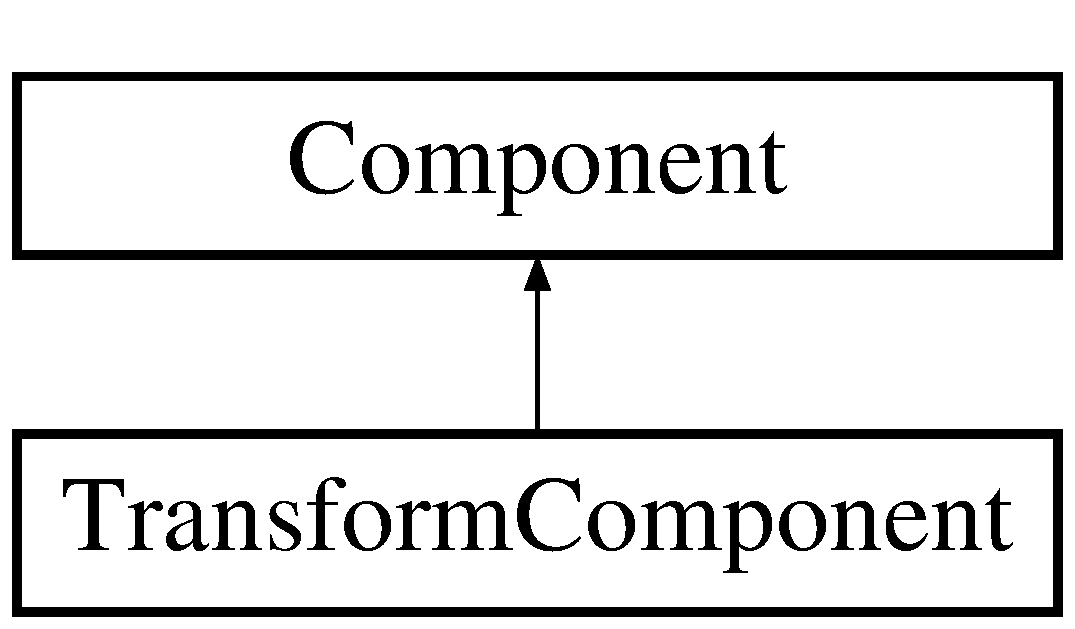
\includegraphics[height=2.000000cm]{class_transform_component}
\end{center}
\end{figure}
\subsection*{Public Member Functions}
\begin{DoxyCompactItemize}
\item 
\mbox{\hyperlink{class_transform_component_ace1cf2d7d2a7468e9cb3eb0ce382f446}{Transform\+Component}} ()
\item 
\mbox{\hyperlink{class_transform_component_a01037615eda19c3bbb51c99094839574}{Transform\+Component}} (const glm\+::vec3 \&pos)
\item 
\mbox{\hyperlink{class_transform_component_a05ce9d2b5a350a5d8d67ce6b323818d4}{Transform\+Component}} (const glm\+::vec3 \&pos, const glm\+::quat \&orient)
\item 
\mbox{\hyperlink{class_transform_component_aa823162adc73870484409dcdb8cc95f3}{Transform\+Component}} (const glm\+::vec3 \&pos, const glm\+::quat \&orient, const glm\+::vec3 \&\mbox{\hyperlink{class_transform_component_a4b04c6a025c6be6bd0b9400827ee2291}{scale}})
\item 
void \mbox{\hyperlink{class_transform_component_ab763f5af77fcb5eee0e725c219901fa3}{On\+Update}} (float dt) override
\item 
void \mbox{\hyperlink{class_transform_component_ac250c4b7e47e639d0f8693d04c9b5051}{On\+Message}} (const std\+::string m) override
\item 
const glm\+::vec3 \& \mbox{\hyperlink{class_transform_component_a1f236ca0fb57ccb2a5e1238502a880ac}{position}} () const
\item 
const glm\+::quat \& \mbox{\hyperlink{class_transform_component_a7655d65aee0cb5dc459e8f632c80a6d1}{orientation}} () const
\item 
const glm\+::vec3 \& \mbox{\hyperlink{class_transform_component_a4b04c6a025c6be6bd0b9400827ee2291}{scale}} () const
\item 
glm\+::mat4 \mbox{\hyperlink{class_transform_component_a5fc531fdaba497dfb2013edce34cb094}{get\+Model\+Matrix}} ()
\item 
void \mbox{\hyperlink{class_transform_component_af6ff15b431e0959b26714037f4b5e5e9}{translate}} (const glm\+::vec3 \&v)
\item 
void \mbox{\hyperlink{class_transform_component_af495b5a63ba61ac9f67170ecf30769ac}{translate}} (float x, float y, float z)
\item 
void \mbox{\hyperlink{class_transform_component_a54f3f0e7924028bb32279aac3938a149}{rotate}} (float angle, const glm\+::vec3 \&axis)
\item 
void \mbox{\hyperlink{class_transform_component_a7c97e7f1e9924b811319acb73accde72}{rotate}} (float angle, float x, float y, float z)
\item 
void \mbox{\hyperlink{class_transform_component_a45483b2f5f38819ad0db6fcfe0f0ded8}{scale\+Up}} (const glm\+::vec3 \&v)
\item 
void \mbox{\hyperlink{class_transform_component_a161374892f674b2e6d34bcaeb66a2a28}{scale\+Up}} (float x, float y, float z)
\item 
void \mbox{\hyperlink{class_transform_component_ae32c6f3f18b81fc712629fb689d61252}{yaw}} (float angle)
\item 
void \mbox{\hyperlink{class_transform_component_ad363ec339461bde470fcc50103d12ba7}{pitch}} (float angle)
\item 
void \mbox{\hyperlink{class_transform_component_ae38356794f70a3838b7c690d3bb0bef7}{roll}} (float angle)
\end{DoxyCompactItemize}
\subsection*{Public Attributes}
\begin{DoxyCompactItemize}
\item 
glm\+::quat \mbox{\hyperlink{class_transform_component_a70f27f66f621e0e52e96e40ec168ede2}{m\+\_\+orientation}}
\end{DoxyCompactItemize}
\subsection*{Protected Attributes}
\begin{DoxyCompactItemize}
\item 
glm\+::vec3 \mbox{\hyperlink{class_transform_component_a5a441b52ff5f18d940e3351e35868481}{m\+\_\+position}}
\item 
glm\+::vec3 \mbox{\hyperlink{class_transform_component_a50d168d6290b29a66b21ce576fa44d59}{m\+\_\+scale}}
\end{DoxyCompactItemize}


\subsection{Detailed Description}
\textbackslash{} class \mbox{\hyperlink{class_this}{This}} component will allow for a game object to be positioned within the game world. 

\subsection{Constructor \& Destructor Documentation}
\mbox{\Hypertarget{class_transform_component_ace1cf2d7d2a7468e9cb3eb0ce382f446}\label{class_transform_component_ace1cf2d7d2a7468e9cb3eb0ce382f446}} 
\index{Transform\+Component@{Transform\+Component}!Transform\+Component@{Transform\+Component}}
\index{Transform\+Component@{Transform\+Component}!Transform\+Component@{Transform\+Component}}
\subsubsection{\texorpdfstring{Transform\+Component()}{TransformComponent()}\hspace{0.1cm}{\footnotesize\ttfamily [1/4]}}
{\footnotesize\ttfamily Transform\+Component\+::\+Transform\+Component (\begin{DoxyParamCaption}{ }\end{DoxyParamCaption})\hspace{0.3cm}{\ttfamily [inline]}}

Constructor \mbox{\Hypertarget{class_transform_component_a01037615eda19c3bbb51c99094839574}\label{class_transform_component_a01037615eda19c3bbb51c99094839574}} 
\index{Transform\+Component@{Transform\+Component}!Transform\+Component@{Transform\+Component}}
\index{Transform\+Component@{Transform\+Component}!Transform\+Component@{Transform\+Component}}
\subsubsection{\texorpdfstring{Transform\+Component()}{TransformComponent()}\hspace{0.1cm}{\footnotesize\ttfamily [2/4]}}
{\footnotesize\ttfamily Transform\+Component\+::\+Transform\+Component (\begin{DoxyParamCaption}\item[{const glm\+::vec3 \&}]{pos }\end{DoxyParamCaption})\hspace{0.3cm}{\ttfamily [inline]}}

Constructor Param One \+: \mbox{\hyperlink{class_the}{The}} position in world space for the connected game object. \mbox{\Hypertarget{class_transform_component_a05ce9d2b5a350a5d8d67ce6b323818d4}\label{class_transform_component_a05ce9d2b5a350a5d8d67ce6b323818d4}} 
\index{Transform\+Component@{Transform\+Component}!Transform\+Component@{Transform\+Component}}
\index{Transform\+Component@{Transform\+Component}!Transform\+Component@{Transform\+Component}}
\subsubsection{\texorpdfstring{Transform\+Component()}{TransformComponent()}\hspace{0.1cm}{\footnotesize\ttfamily [3/4]}}
{\footnotesize\ttfamily Transform\+Component\+::\+Transform\+Component (\begin{DoxyParamCaption}\item[{const glm\+::vec3 \&}]{pos,  }\item[{const glm\+::quat \&}]{orient }\end{DoxyParamCaption})\hspace{0.3cm}{\ttfamily [inline]}}

Constructor Param One \+: \mbox{\hyperlink{class_the}{The}} position in world space for the connected game object. Param Two \+: \mbox{\hyperlink{class_the}{The}} direction the game object is facing. \mbox{\Hypertarget{class_transform_component_aa823162adc73870484409dcdb8cc95f3}\label{class_transform_component_aa823162adc73870484409dcdb8cc95f3}} 
\index{Transform\+Component@{Transform\+Component}!Transform\+Component@{Transform\+Component}}
\index{Transform\+Component@{Transform\+Component}!Transform\+Component@{Transform\+Component}}
\subsubsection{\texorpdfstring{Transform\+Component()}{TransformComponent()}\hspace{0.1cm}{\footnotesize\ttfamily [4/4]}}
{\footnotesize\ttfamily Transform\+Component\+::\+Transform\+Component (\begin{DoxyParamCaption}\item[{const glm\+::vec3 \&}]{pos,  }\item[{const glm\+::quat \&}]{orient,  }\item[{const glm\+::vec3 \&}]{scale }\end{DoxyParamCaption})\hspace{0.3cm}{\ttfamily [inline]}}

Constructor Param One \+: \mbox{\hyperlink{class_the}{The}} position in world space for the connected game object. Param Two \+: \mbox{\hyperlink{class_the}{The}} direction the game object is facing. Param Three \+: \mbox{\hyperlink{class_the}{The}} scaled size of the game object. 

\subsection{Member Function Documentation}
\mbox{\Hypertarget{class_transform_component_a5fc531fdaba497dfb2013edce34cb094}\label{class_transform_component_a5fc531fdaba497dfb2013edce34cb094}} 
\index{Transform\+Component@{Transform\+Component}!get\+Model\+Matrix@{get\+Model\+Matrix}}
\index{get\+Model\+Matrix@{get\+Model\+Matrix}!Transform\+Component@{Transform\+Component}}
\subsubsection{\texorpdfstring{get\+Model\+Matrix()}{getModelMatrix()}}
{\footnotesize\ttfamily glm\+::mat4 Transform\+Component\+::get\+Model\+Matrix (\begin{DoxyParamCaption}{ }\end{DoxyParamCaption})\hspace{0.3cm}{\ttfamily [inline]}}

Get\+Model\+Matrix \+: \mbox{\hyperlink{class_this}{This}} will use the current transform data to form a complete model matrix allowing for the game object to be drawn. \mbox{\Hypertarget{class_transform_component_ac250c4b7e47e639d0f8693d04c9b5051}\label{class_transform_component_ac250c4b7e47e639d0f8693d04c9b5051}} 
\index{Transform\+Component@{Transform\+Component}!On\+Message@{On\+Message}}
\index{On\+Message@{On\+Message}!Transform\+Component@{Transform\+Component}}
\subsubsection{\texorpdfstring{On\+Message()}{OnMessage()}}
{\footnotesize\ttfamily void Transform\+Component\+::\+On\+Message (\begin{DoxyParamCaption}\item[{const std\+::string}]{m }\end{DoxyParamCaption})\hspace{0.3cm}{\ttfamily [inline]}, {\ttfamily [override]}, {\ttfamily [virtual]}}

On\+Message \+: \mbox{\hyperlink{class_this}{This}} will allow for the component to respond to a key press. 

Implements \mbox{\hyperlink{class_component_a1a880fe5e212cd7ef8241e220660417d}{Component}}.

\mbox{\Hypertarget{class_transform_component_ab763f5af77fcb5eee0e725c219901fa3}\label{class_transform_component_ab763f5af77fcb5eee0e725c219901fa3}} 
\index{Transform\+Component@{Transform\+Component}!On\+Update@{On\+Update}}
\index{On\+Update@{On\+Update}!Transform\+Component@{Transform\+Component}}
\subsubsection{\texorpdfstring{On\+Update()}{OnUpdate()}}
{\footnotesize\ttfamily void Transform\+Component\+::\+On\+Update (\begin{DoxyParamCaption}\item[{float}]{dt }\end{DoxyParamCaption})\hspace{0.3cm}{\ttfamily [inline]}, {\ttfamily [override]}, {\ttfamily [virtual]}}

On\+Update \+: \mbox{\hyperlink{class_this}{This}} will be used to update this component. 

Implements \mbox{\hyperlink{class_component_ab71d7f4b6d8792287a9b0c9e045acbe0}{Component}}.

\mbox{\Hypertarget{class_transform_component_a7655d65aee0cb5dc459e8f632c80a6d1}\label{class_transform_component_a7655d65aee0cb5dc459e8f632c80a6d1}} 
\index{Transform\+Component@{Transform\+Component}!orientation@{orientation}}
\index{orientation@{orientation}!Transform\+Component@{Transform\+Component}}
\subsubsection{\texorpdfstring{orientation()}{orientation()}}
{\footnotesize\ttfamily const glm\+::quat\& Transform\+Component\+::orientation (\begin{DoxyParamCaption}{ }\end{DoxyParamCaption}) const\hspace{0.3cm}{\ttfamily [inline]}}

Orientation \+: \mbox{\hyperlink{class_this}{This}} will return the current direction the game object is facing. \mbox{\Hypertarget{class_transform_component_ad363ec339461bde470fcc50103d12ba7}\label{class_transform_component_ad363ec339461bde470fcc50103d12ba7}} 
\index{Transform\+Component@{Transform\+Component}!pitch@{pitch}}
\index{pitch@{pitch}!Transform\+Component@{Transform\+Component}}
\subsubsection{\texorpdfstring{pitch()}{pitch()}}
{\footnotesize\ttfamily void Transform\+Component\+::pitch (\begin{DoxyParamCaption}\item[{float}]{angle }\end{DoxyParamCaption})\hspace{0.3cm}{\ttfamily [inline]}}

Pitch \+: \mbox{\hyperlink{class_this}{This}} will rotate the game object by the angle around the Y-\/\+Axis. Param One \+: \mbox{\hyperlink{class_the}{The}} angle of which to rotate by. \mbox{\Hypertarget{class_transform_component_a1f236ca0fb57ccb2a5e1238502a880ac}\label{class_transform_component_a1f236ca0fb57ccb2a5e1238502a880ac}} 
\index{Transform\+Component@{Transform\+Component}!position@{position}}
\index{position@{position}!Transform\+Component@{Transform\+Component}}
\subsubsection{\texorpdfstring{position()}{position()}}
{\footnotesize\ttfamily const glm\+::vec3\& Transform\+Component\+::position (\begin{DoxyParamCaption}{ }\end{DoxyParamCaption}) const\hspace{0.3cm}{\ttfamily [inline]}}

Position \+: \mbox{\hyperlink{class_this}{This}} will be used to return the value of position. \mbox{\Hypertarget{class_transform_component_ae38356794f70a3838b7c690d3bb0bef7}\label{class_transform_component_ae38356794f70a3838b7c690d3bb0bef7}} 
\index{Transform\+Component@{Transform\+Component}!roll@{roll}}
\index{roll@{roll}!Transform\+Component@{Transform\+Component}}
\subsubsection{\texorpdfstring{roll()}{roll()}}
{\footnotesize\ttfamily void Transform\+Component\+::roll (\begin{DoxyParamCaption}\item[{float}]{angle }\end{DoxyParamCaption})\hspace{0.3cm}{\ttfamily [inline]}}

Roll \+: \mbox{\hyperlink{class_this}{This}} will rotate the game object by the angle around the X-\/\+Axis. Param One \+: \mbox{\hyperlink{class_the}{The}} angle of which to rotate by. \mbox{\Hypertarget{class_transform_component_a54f3f0e7924028bb32279aac3938a149}\label{class_transform_component_a54f3f0e7924028bb32279aac3938a149}} 
\index{Transform\+Component@{Transform\+Component}!rotate@{rotate}}
\index{rotate@{rotate}!Transform\+Component@{Transform\+Component}}
\subsubsection{\texorpdfstring{rotate()}{rotate()}\hspace{0.1cm}{\footnotesize\ttfamily [1/2]}}
{\footnotesize\ttfamily void Transform\+Component\+::rotate (\begin{DoxyParamCaption}\item[{float}]{angle,  }\item[{const glm\+::vec3 \&}]{axis }\end{DoxyParamCaption})\hspace{0.3cm}{\ttfamily [inline]}}

Rotate \+: \mbox{\hyperlink{class_this}{This}} will rotate the game object around a single axis. Param One \+: \mbox{\hyperlink{class_the}{The}} angle of whic to rotate by. Param Two \+: \mbox{\hyperlink{class_the}{The}} fixed axix to rotate the object around. \mbox{\Hypertarget{class_transform_component_a7c97e7f1e9924b811319acb73accde72}\label{class_transform_component_a7c97e7f1e9924b811319acb73accde72}} 
\index{Transform\+Component@{Transform\+Component}!rotate@{rotate}}
\index{rotate@{rotate}!Transform\+Component@{Transform\+Component}}
\subsubsection{\texorpdfstring{rotate()}{rotate()}\hspace{0.1cm}{\footnotesize\ttfamily [2/2]}}
{\footnotesize\ttfamily void Transform\+Component\+::rotate (\begin{DoxyParamCaption}\item[{float}]{angle,  }\item[{float}]{x,  }\item[{float}]{y,  }\item[{float}]{z }\end{DoxyParamCaption})\hspace{0.3cm}{\ttfamily [inline]}}

Rotate \+: \mbox{\hyperlink{class_this}{This}} will rotate the game object around a single axis. Param One \+: \mbox{\hyperlink{class_the}{The}} angle of whic to rotate by. Param Two \+: \mbox{\hyperlink{class_the}{The}} X for the fixed axix to rotate the object around. Param Three \+: \+: \mbox{\hyperlink{class_the}{The}} Y for the fixed axix to rotate the object around. Param Four \+: \mbox{\hyperlink{class_the}{The}} Z for the fixed axix to rotate the object around. \mbox{\Hypertarget{class_transform_component_a4b04c6a025c6be6bd0b9400827ee2291}\label{class_transform_component_a4b04c6a025c6be6bd0b9400827ee2291}} 
\index{Transform\+Component@{Transform\+Component}!scale@{scale}}
\index{scale@{scale}!Transform\+Component@{Transform\+Component}}
\subsubsection{\texorpdfstring{scale()}{scale()}}
{\footnotesize\ttfamily const glm\+::vec3\& Transform\+Component\+::scale (\begin{DoxyParamCaption}{ }\end{DoxyParamCaption}) const\hspace{0.3cm}{\ttfamily [inline]}}

Scale \+: \mbox{\hyperlink{class_this}{This}} will return the current scale factor for the game object. \mbox{\Hypertarget{class_transform_component_a45483b2f5f38819ad0db6fcfe0f0ded8}\label{class_transform_component_a45483b2f5f38819ad0db6fcfe0f0ded8}} 
\index{Transform\+Component@{Transform\+Component}!scale\+Up@{scale\+Up}}
\index{scale\+Up@{scale\+Up}!Transform\+Component@{Transform\+Component}}
\subsubsection{\texorpdfstring{scale\+Up()}{scaleUp()}\hspace{0.1cm}{\footnotesize\ttfamily [1/2]}}
{\footnotesize\ttfamily void Transform\+Component\+::scale\+Up (\begin{DoxyParamCaption}\item[{const glm\+::vec3 \&}]{v }\end{DoxyParamCaption})\hspace{0.3cm}{\ttfamily [inline]}}

Scale\+Up \+: \mbox{\hyperlink{class_this}{This}} will increate the scale of the game object by \textquotesingle{}v\textquotesingle{}. Param One \+: A set of value of which to scale the object by. \mbox{\Hypertarget{class_transform_component_a161374892f674b2e6d34bcaeb66a2a28}\label{class_transform_component_a161374892f674b2e6d34bcaeb66a2a28}} 
\index{Transform\+Component@{Transform\+Component}!scale\+Up@{scale\+Up}}
\index{scale\+Up@{scale\+Up}!Transform\+Component@{Transform\+Component}}
\subsubsection{\texorpdfstring{scale\+Up()}{scaleUp()}\hspace{0.1cm}{\footnotesize\ttfamily [2/2]}}
{\footnotesize\ttfamily void Transform\+Component\+::scale\+Up (\begin{DoxyParamCaption}\item[{float}]{x,  }\item[{float}]{y,  }\item[{float}]{z }\end{DoxyParamCaption})\hspace{0.3cm}{\ttfamily [inline]}}

Scale\+Up \+: \mbox{\hyperlink{class_this}{This}} will increate the scale of the game object by \textquotesingle{}v\textquotesingle{}. Param One \+: \mbox{\hyperlink{class_the}{The}} value of which to scale the object in the X axis. Param Two \+: \mbox{\hyperlink{class_the}{The}} value of which to scale the object in the Y axis. Param Three \+: \mbox{\hyperlink{class_the}{The}} value of which to scale the object in the Z axis. \mbox{\Hypertarget{class_transform_component_af6ff15b431e0959b26714037f4b5e5e9}\label{class_transform_component_af6ff15b431e0959b26714037f4b5e5e9}} 
\index{Transform\+Component@{Transform\+Component}!translate@{translate}}
\index{translate@{translate}!Transform\+Component@{Transform\+Component}}
\subsubsection{\texorpdfstring{translate()}{translate()}\hspace{0.1cm}{\footnotesize\ttfamily [1/2]}}
{\footnotesize\ttfamily void Transform\+Component\+::translate (\begin{DoxyParamCaption}\item[{const glm\+::vec3 \&}]{v }\end{DoxyParamCaption})\hspace{0.3cm}{\ttfamily [inline]}}

Translate \+: \mbox{\hyperlink{class_this}{This}} will move the connected game object by the value of \textquotesingle{}v\textquotesingle{} Param One \+: a set of coordinate of which to move the object by. \mbox{\Hypertarget{class_transform_component_af495b5a63ba61ac9f67170ecf30769ac}\label{class_transform_component_af495b5a63ba61ac9f67170ecf30769ac}} 
\index{Transform\+Component@{Transform\+Component}!translate@{translate}}
\index{translate@{translate}!Transform\+Component@{Transform\+Component}}
\subsubsection{\texorpdfstring{translate()}{translate()}\hspace{0.1cm}{\footnotesize\ttfamily [2/2]}}
{\footnotesize\ttfamily void Transform\+Component\+::translate (\begin{DoxyParamCaption}\item[{float}]{x,  }\item[{float}]{y,  }\item[{float}]{z }\end{DoxyParamCaption})\hspace{0.3cm}{\ttfamily [inline]}}

Translate \+: \mbox{\hyperlink{class_this}{This}} will move the game objtect by an x, y, z vlaue. Param One \+: \mbox{\hyperlink{class_the}{The}} X value to move. Param Two \+: \mbox{\hyperlink{class_the}{The}} Y vlaue to move. Param Three \+: \mbox{\hyperlink{class_the}{The}} Z value to move. \mbox{\Hypertarget{class_transform_component_ae32c6f3f18b81fc712629fb689d61252}\label{class_transform_component_ae32c6f3f18b81fc712629fb689d61252}} 
\index{Transform\+Component@{Transform\+Component}!yaw@{yaw}}
\index{yaw@{yaw}!Transform\+Component@{Transform\+Component}}
\subsubsection{\texorpdfstring{yaw()}{yaw()}}
{\footnotesize\ttfamily void Transform\+Component\+::yaw (\begin{DoxyParamCaption}\item[{float}]{angle }\end{DoxyParamCaption})\hspace{0.3cm}{\ttfamily [inline]}}

Yaw \+: \mbox{\hyperlink{class_this}{This}} will rotate the game object by the angle around the Z-\/\+Axis. Param One \+: \mbox{\hyperlink{class_the}{The}} angle of which to rotate by. 

\subsection{Member Data Documentation}
\mbox{\Hypertarget{class_transform_component_a70f27f66f621e0e52e96e40ec168ede2}\label{class_transform_component_a70f27f66f621e0e52e96e40ec168ede2}} 
\index{Transform\+Component@{Transform\+Component}!m\+\_\+orientation@{m\+\_\+orientation}}
\index{m\+\_\+orientation@{m\+\_\+orientation}!Transform\+Component@{Transform\+Component}}
\subsubsection{\texorpdfstring{m\+\_\+orientation}{m\_orientation}}
{\footnotesize\ttfamily glm\+::quat Transform\+Component\+::m\+\_\+orientation}

\mbox{\Hypertarget{class_transform_component_a5a441b52ff5f18d940e3351e35868481}\label{class_transform_component_a5a441b52ff5f18d940e3351e35868481}} 
\index{Transform\+Component@{Transform\+Component}!m\+\_\+position@{m\+\_\+position}}
\index{m\+\_\+position@{m\+\_\+position}!Transform\+Component@{Transform\+Component}}
\subsubsection{\texorpdfstring{m\+\_\+position}{m\_position}}
{\footnotesize\ttfamily glm\+::vec3 Transform\+Component\+::m\+\_\+position\hspace{0.3cm}{\ttfamily [protected]}}

\mbox{\Hypertarget{class_transform_component_a50d168d6290b29a66b21ce576fa44d59}\label{class_transform_component_a50d168d6290b29a66b21ce576fa44d59}} 
\index{Transform\+Component@{Transform\+Component}!m\+\_\+scale@{m\+\_\+scale}}
\index{m\+\_\+scale@{m\+\_\+scale}!Transform\+Component@{Transform\+Component}}
\subsubsection{\texorpdfstring{m\+\_\+scale}{m\_scale}}
{\footnotesize\ttfamily glm\+::vec3 Transform\+Component\+::m\+\_\+scale\hspace{0.3cm}{\ttfamily [protected]}}



The documentation for this class was generated from the following file\+:\begin{DoxyCompactItemize}
\item 
Game\+Engine/include/\mbox{\hyperlink{_transform_component_8h}{Transform\+Component.\+h}}\end{DoxyCompactItemize}

\hypertarget{class_used}{}\section{Used Class Reference}
\label{class_used}\index{Used@{Used}}


\subsection{Detailed Description}
the player. 

The documentation for this class was generated from the following file\+:\begin{DoxyCompactItemize}
\item 
Game\+Engine/include/\mbox{\hyperlink{_input_handler_8h}{Input\+Handler.\+h}}\end{DoxyCompactItemize}

\hypertarget{struct_vertex}{}\section{Vertex Struct Reference}
\label{struct_vertex}\index{Vertex@{Vertex}}


{\ttfamily \#include $<$Mesh.\+h$>$}

\subsection*{Public Attributes}
\begin{DoxyCompactItemize}
\item 
glm\+::vec3 \mbox{\hyperlink{struct_vertex_a030819fdc241743bbd3e180a6b132ed3}{position}}
\item 
glm\+::vec3 \mbox{\hyperlink{struct_vertex_a3aa35fe84025ecf1acccb5f65f5577fd}{normal}}
\item 
glm\+::vec2 \mbox{\hyperlink{struct_vertex_a03ba1fdd25400383cd40bd2153d08ef1}{texture\+Coords}}
\end{DoxyCompactItemize}


\subsection{Member Data Documentation}
\mbox{\Hypertarget{struct_vertex_a3aa35fe84025ecf1acccb5f65f5577fd}\label{struct_vertex_a3aa35fe84025ecf1acccb5f65f5577fd}} 
\index{Vertex@{Vertex}!normal@{normal}}
\index{normal@{normal}!Vertex@{Vertex}}
\subsubsection{\texorpdfstring{normal}{normal}}
{\footnotesize\ttfamily glm\+::vec3 Vertex\+::normal}

\mbox{\Hypertarget{struct_vertex_a030819fdc241743bbd3e180a6b132ed3}\label{struct_vertex_a030819fdc241743bbd3e180a6b132ed3}} 
\index{Vertex@{Vertex}!position@{position}}
\index{position@{position}!Vertex@{Vertex}}
\subsubsection{\texorpdfstring{position}{position}}
{\footnotesize\ttfamily glm\+::vec3 Vertex\+::position}

\mbox{\Hypertarget{struct_vertex_a03ba1fdd25400383cd40bd2153d08ef1}\label{struct_vertex_a03ba1fdd25400383cd40bd2153d08ef1}} 
\index{Vertex@{Vertex}!texture\+Coords@{texture\+Coords}}
\index{texture\+Coords@{texture\+Coords}!Vertex@{Vertex}}
\subsubsection{\texorpdfstring{texture\+Coords}{textureCoords}}
{\footnotesize\ttfamily glm\+::vec2 Vertex\+::texture\+Coords}



The documentation for this struct was generated from the following file\+:\begin{DoxyCompactItemize}
\item 
Game\+Engine/include/\mbox{\hyperlink{_mesh_8h}{Mesh.\+h}}\end{DoxyCompactItemize}

\chapter{File Documentation}
\hypertarget{_camera_8h}{}\section{Game\+Engine/include/\+Camera.h File Reference}
\label{_camera_8h}\index{Game\+Engine/include/\+Camera.\+h@{Game\+Engine/include/\+Camera.\+h}}
{\ttfamily \#include $<$glm/glm.\+hpp$>$}\newline
{\ttfamily \#include $<$glm/gtc/matrix\+\_\+transform.\+hpp$>$}\newline
{\ttfamily \#include $<$glm/gtc/type\+\_\+ptr.\+hpp$>$}\newline
{\ttfamily \#include $<$glm/gtx/quaternion.\+hpp$>$}\newline
\subsection*{Classes}
\begin{DoxyCompactItemize}
\item 
class \mbox{\hyperlink{class_camera}{Camera}}
\end{DoxyCompactItemize}
\subsection*{Macros}
\begin{DoxyCompactItemize}
\item 
\#define \mbox{\hyperlink{_camera_8h_abd75661fe7969e19439052a5f69ba5d1}{G\+L\+M\+\_\+\+E\+N\+A\+B\+L\+E\+\_\+\+E\+X\+P\+E\+R\+I\+M\+E\+N\+T\+AL}}
\end{DoxyCompactItemize}


\subsection{Macro Definition Documentation}
\mbox{\Hypertarget{_camera_8h_abd75661fe7969e19439052a5f69ba5d1}\label{_camera_8h_abd75661fe7969e19439052a5f69ba5d1}} 
\index{Camera.\+h@{Camera.\+h}!G\+L\+M\+\_\+\+E\+N\+A\+B\+L\+E\+\_\+\+E\+X\+P\+E\+R\+I\+M\+E\+N\+T\+AL@{G\+L\+M\+\_\+\+E\+N\+A\+B\+L\+E\+\_\+\+E\+X\+P\+E\+R\+I\+M\+E\+N\+T\+AL}}
\index{G\+L\+M\+\_\+\+E\+N\+A\+B\+L\+E\+\_\+\+E\+X\+P\+E\+R\+I\+M\+E\+N\+T\+AL@{G\+L\+M\+\_\+\+E\+N\+A\+B\+L\+E\+\_\+\+E\+X\+P\+E\+R\+I\+M\+E\+N\+T\+AL}!Camera.\+h@{Camera.\+h}}
\subsubsection{\texorpdfstring{G\+L\+M\+\_\+\+E\+N\+A\+B\+L\+E\+\_\+\+E\+X\+P\+E\+R\+I\+M\+E\+N\+T\+AL}{GLM\_ENABLE\_EXPERIMENTAL}}
{\footnotesize\ttfamily \#define G\+L\+M\+\_\+\+E\+N\+A\+B\+L\+E\+\_\+\+E\+X\+P\+E\+R\+I\+M\+E\+N\+T\+AL}


\hypertarget{_camera_component_8h}{}\section{Game\+Engine/include/\+Camera\+Component.h File Reference}
\label{_camera_component_8h}\index{Game\+Engine/include/\+Camera\+Component.\+h@{Game\+Engine/include/\+Camera\+Component.\+h}}
{\ttfamily \#include \char`\"{}Component.\+h\char`\"{}}\newline
{\ttfamily \#include \char`\"{}Game\+Object.\+h\char`\"{}}\newline
{\ttfamily \#include \char`\"{}Camera.\+h\char`\"{}}\newline
\subsection*{Classes}
\begin{DoxyCompactItemize}
\item 
class \mbox{\hyperlink{class_camera_component}{Camera\+Component}}
\end{DoxyCompactItemize}
\subsection*{Macros}
\begin{DoxyCompactItemize}
\item 
\#define \mbox{\hyperlink{_camera_component_8h_aa1445031ea657765e5caa3d1236d54f2}{R\+O\+T\+A\+T\+I\+O\+N\+\_\+\+V\+A\+L\+UE}}~0.\+005f
\end{DoxyCompactItemize}
\subsection*{Enumerations}
\begin{DoxyCompactItemize}
\item 
enum \mbox{\hyperlink{_camera_component_8h_ab07ecb557631c59d8b7ec9c3db110dd5}{camera\+Type}} \{ \mbox{\hyperlink{_camera_component_8h_ab07ecb557631c59d8b7ec9c3db110dd5aa9e95148c5a271e009cbee071b3fdaa9}{static\+Camera}} = 0x300, 
\mbox{\hyperlink{_camera_component_8h_ab07ecb557631c59d8b7ec9c3db110dd5a75322cf4d7e797fe57f13e689154bf89}{third\+Person\+Camera}} = 0x400, 
\mbox{\hyperlink{_camera_component_8h_ab07ecb557631c59d8b7ec9c3db110dd5a5998f09ea3884c99259a52a8a00db0bb}{first\+Person\+Camera}} = 0x500
 \}
\end{DoxyCompactItemize}


\subsection{Macro Definition Documentation}
\mbox{\Hypertarget{_camera_component_8h_aa1445031ea657765e5caa3d1236d54f2}\label{_camera_component_8h_aa1445031ea657765e5caa3d1236d54f2}} 
\index{Camera\+Component.\+h@{Camera\+Component.\+h}!R\+O\+T\+A\+T\+I\+O\+N\+\_\+\+V\+A\+L\+UE@{R\+O\+T\+A\+T\+I\+O\+N\+\_\+\+V\+A\+L\+UE}}
\index{R\+O\+T\+A\+T\+I\+O\+N\+\_\+\+V\+A\+L\+UE@{R\+O\+T\+A\+T\+I\+O\+N\+\_\+\+V\+A\+L\+UE}!Camera\+Component.\+h@{Camera\+Component.\+h}}
\subsubsection{\texorpdfstring{R\+O\+T\+A\+T\+I\+O\+N\+\_\+\+V\+A\+L\+UE}{ROTATION\_VALUE}}
{\footnotesize\ttfamily \#define R\+O\+T\+A\+T\+I\+O\+N\+\_\+\+V\+A\+L\+UE~0.\+005f}



\subsection{Enumeration Type Documentation}
\mbox{\Hypertarget{_camera_component_8h_ab07ecb557631c59d8b7ec9c3db110dd5}\label{_camera_component_8h_ab07ecb557631c59d8b7ec9c3db110dd5}} 
\index{Camera\+Component.\+h@{Camera\+Component.\+h}!camera\+Type@{camera\+Type}}
\index{camera\+Type@{camera\+Type}!Camera\+Component.\+h@{Camera\+Component.\+h}}
\subsubsection{\texorpdfstring{camera\+Type}{cameraType}}
{\footnotesize\ttfamily enum \mbox{\hyperlink{_camera_component_8h_ab07ecb557631c59d8b7ec9c3db110dd5}{camera\+Type}}}

\begin{DoxyEnumFields}{Enumerator}
\raisebox{\heightof{T}}[0pt][0pt]{\index{static\+Camera@{static\+Camera}!Camera\+Component.\+h@{Camera\+Component.\+h}}\index{Camera\+Component.\+h@{Camera\+Component.\+h}!static\+Camera@{static\+Camera}}}\mbox{\Hypertarget{_camera_component_8h_ab07ecb557631c59d8b7ec9c3db110dd5aa9e95148c5a271e009cbee071b3fdaa9}\label{_camera_component_8h_ab07ecb557631c59d8b7ec9c3db110dd5aa9e95148c5a271e009cbee071b3fdaa9}} 
static\+Camera&\\
\hline

\raisebox{\heightof{T}}[0pt][0pt]{\index{third\+Person\+Camera@{third\+Person\+Camera}!Camera\+Component.\+h@{Camera\+Component.\+h}}\index{Camera\+Component.\+h@{Camera\+Component.\+h}!third\+Person\+Camera@{third\+Person\+Camera}}}\mbox{\Hypertarget{_camera_component_8h_ab07ecb557631c59d8b7ec9c3db110dd5a75322cf4d7e797fe57f13e689154bf89}\label{_camera_component_8h_ab07ecb557631c59d8b7ec9c3db110dd5a75322cf4d7e797fe57f13e689154bf89}} 
third\+Person\+Camera&\\
\hline

\raisebox{\heightof{T}}[0pt][0pt]{\index{first\+Person\+Camera@{first\+Person\+Camera}!Camera\+Component.\+h@{Camera\+Component.\+h}}\index{Camera\+Component.\+h@{Camera\+Component.\+h}!first\+Person\+Camera@{first\+Person\+Camera}}}\mbox{\Hypertarget{_camera_component_8h_ab07ecb557631c59d8b7ec9c3db110dd5a5998f09ea3884c99259a52a8a00db0bb}\label{_camera_component_8h_ab07ecb557631c59d8b7ec9c3db110dd5a5998f09ea3884c99259a52a8a00db0bb}} 
first\+Person\+Camera&\\
\hline

\end{DoxyEnumFields}

\hypertarget{_colour_component_8h}{}\section{Game\+Engine/include/\+Colour\+Component.h File Reference}
\label{_colour_component_8h}\index{Game\+Engine/include/\+Colour\+Component.\+h@{Game\+Engine/include/\+Colour\+Component.\+h}}
{\ttfamily \#include \char`\"{}Component.\+h\char`\"{}}\newline
\subsection*{Classes}
\begin{DoxyCompactItemize}
\item 
class \mbox{\hyperlink{class_colour_component}{Colour\+Component}}
\item 
class \mbox{\hyperlink{class_red_component}{Red\+Component}}
\item 
class \mbox{\hyperlink{class_green_component}{Green\+Component}}
\item 
class \mbox{\hyperlink{class_blue_component}{Blue\+Component}}
\end{DoxyCompactItemize}
\subsection*{Macros}
\begin{DoxyCompactItemize}
\item 
\#define \mbox{\hyperlink{_colour_component_8h_a64a0af262d0d872f48330da6157cf022}{C\+O\+L\+O\+U\+R\+\_\+\+A\+D\+J\+U\+S\+T\+M\+E\+N\+T\+\_\+\+V\+A\+L\+UE}}~0.\+001f
\end{DoxyCompactItemize}


\subsection{Macro Definition Documentation}
\mbox{\Hypertarget{_colour_component_8h_a64a0af262d0d872f48330da6157cf022}\label{_colour_component_8h_a64a0af262d0d872f48330da6157cf022}} 
\index{Colour\+Component.\+h@{Colour\+Component.\+h}!C\+O\+L\+O\+U\+R\+\_\+\+A\+D\+J\+U\+S\+T\+M\+E\+N\+T\+\_\+\+V\+A\+L\+UE@{C\+O\+L\+O\+U\+R\+\_\+\+A\+D\+J\+U\+S\+T\+M\+E\+N\+T\+\_\+\+V\+A\+L\+UE}}
\index{C\+O\+L\+O\+U\+R\+\_\+\+A\+D\+J\+U\+S\+T\+M\+E\+N\+T\+\_\+\+V\+A\+L\+UE@{C\+O\+L\+O\+U\+R\+\_\+\+A\+D\+J\+U\+S\+T\+M\+E\+N\+T\+\_\+\+V\+A\+L\+UE}!Colour\+Component.\+h@{Colour\+Component.\+h}}
\subsubsection{\texorpdfstring{C\+O\+L\+O\+U\+R\+\_\+\+A\+D\+J\+U\+S\+T\+M\+E\+N\+T\+\_\+\+V\+A\+L\+UE}{COLOUR\_ADJUSTMENT\_VALUE}}
{\footnotesize\ttfamily \#define C\+O\+L\+O\+U\+R\+\_\+\+A\+D\+J\+U\+S\+T\+M\+E\+N\+T\+\_\+\+V\+A\+L\+UE~0.\+001f}


\hypertarget{_component_8h}{}\section{Game\+Engine/include/\+Component.h File Reference}
\label{_component_8h}\index{Game\+Engine/include/\+Component.\+h@{Game\+Engine/include/\+Component.\+h}}
{\ttfamily \#include $<$string$>$}\newline
\subsection*{Classes}
\begin{DoxyCompactItemize}
\item 
class \mbox{\hyperlink{class_component}{Component}}
\end{DoxyCompactItemize}

\hypertarget{_game_8h}{}\section{Game\+Engine/include/\+Game.h File Reference}
\label{_game_8h}\index{Game\+Engine/include/\+Game.\+h@{Game\+Engine/include/\+Game.\+h}}
{\ttfamily \#include $<$G\+L\+A\+D/glad.\+h$>$}\newline
{\ttfamily \#include $<$G\+L\+F\+W/glfw3.\+h$>$}\newline
{\ttfamily \#include \char`\"{}I\+Engine\+Core.\+h\char`\"{}}\newline
{\ttfamily \#include \char`\"{}Input\+Handler.\+h\char`\"{}}\newline
{\ttfamily \#include \char`\"{}Game\+Object.\+h\char`\"{}}\newline
{\ttfamily \#include \char`\"{}Camera.\+h\char`\"{}}\newline
{\ttfamily \#include \char`\"{}Scene.\+h\char`\"{}}\newline
{\ttfamily \#include \char`\"{}Renderer.\+h\char`\"{}}\newline
{\ttfamily \#include \char`\"{}Game\+Manager.\+h\char`\"{}}\newline
\subsection*{Classes}
\begin{DoxyCompactItemize}
\item 
class \mbox{\hyperlink{class_game}{Game}}
\end{DoxyCompactItemize}

\hypertarget{_game_manager_8h}{}\section{Game\+Engine/include/\+Game\+Manager.h File Reference}
\label{_game_manager_8h}\index{Game\+Engine/include/\+Game\+Manager.\+h@{Game\+Engine/include/\+Game\+Manager.\+h}}
{\ttfamily \#include \char`\"{}Game\+Object.\+h\char`\"{}}\newline
{\ttfamily \#include \char`\"{}Transform\+Component.\+h\char`\"{}}\newline
{\ttfamily \#include \char`\"{}Move\+Component.\+h\char`\"{}}\newline
{\ttfamily \#include \char`\"{}Camera\+Component.\+h\char`\"{}}\newline
{\ttfamily \#include \char`\"{}Model.\+h\char`\"{}}\newline
{\ttfamily \#include \char`\"{}Model\+Component.\+h\char`\"{}}\newline
\subsection*{Classes}
\begin{DoxyCompactItemize}
\item 
class \mbox{\hyperlink{class_game_manager}{Game\+Manager}}
\end{DoxyCompactItemize}

\hypertarget{_game_object_8h}{}\section{Game\+Engine/include/\+Game\+Object.h File Reference}
\label{_game_object_8h}\index{Game\+Engine/include/\+Game\+Object.\+h@{Game\+Engine/include/\+Game\+Object.\+h}}
{\ttfamily \#include $<$unordered\+\_\+map$>$}\newline
{\ttfamily \#include $<$typeindex$>$}\newline
{\ttfamily \#include \char`\"{}Component.\+h\char`\"{}}\newline
\subsection*{Classes}
\begin{DoxyCompactItemize}
\item 
class \mbox{\hyperlink{class_game_object}{Game\+Object}}
\end{DoxyCompactItemize}

\hypertarget{_g_l_f_w___engine_core_8h}{}\section{Game\+Engine/include/\+G\+L\+F\+W\+\_\+\+Engine\+Core.h File Reference}
\label{_g_l_f_w___engine_core_8h}\index{Game\+Engine/include/\+G\+L\+F\+W\+\_\+\+Engine\+Core.\+h@{Game\+Engine/include/\+G\+L\+F\+W\+\_\+\+Engine\+Core.\+h}}
{\ttfamily \#include \char`\"{}I\+Engine\+Core.\+h\char`\"{}}\newline
{\ttfamily \#include $<$G\+L\+A\+D/glad.\+h$>$}\newline
{\ttfamily \#include $<$G\+L\+F\+W/glfw3.\+h$>$}\newline
{\ttfamily \#include $<$vector$>$}\newline
{\ttfamily \#include $<$glm/mat4x4.\+hpp$>$}\newline
{\ttfamily \#include \char`\"{}Camera.\+h\char`\"{}}\newline
{\ttfamily \#include \char`\"{}Model.\+h\char`\"{}}\newline
\subsection*{Classes}
\begin{DoxyCompactItemize}
\item 
class \mbox{\hyperlink{class_g_l_f_w___engine_core}{G\+L\+F\+W\+\_\+\+Engine\+Core}}
\end{DoxyCompactItemize}

\hypertarget{_i_engine_core_8h}{}\section{Game\+Engine/include/\+I\+Engine\+Core.h File Reference}
\label{_i_engine_core_8h}\index{Game\+Engine/include/\+I\+Engine\+Core.\+h@{Game\+Engine/include/\+I\+Engine\+Core.\+h}}
{\ttfamily \#include $<$string$>$}\newline
{\ttfamily \#include $<$iostream$>$}\newline
{\ttfamily \#include $<$glm/mat4x4.\+hpp$>$}\newline
{\ttfamily \#include \char`\"{}Model.\+h\char`\"{}}\newline
\subsection*{Classes}
\begin{DoxyCompactItemize}
\item 
class \mbox{\hyperlink{class_i_engine_core}{I\+Engine\+Core}}
\end{DoxyCompactItemize}

\hypertarget{_input_handler_8h}{}\section{Game\+Engine/include/\+Input\+Handler.h File Reference}
\label{_input_handler_8h}\index{Game\+Engine/include/\+Input\+Handler.\+h@{Game\+Engine/include/\+Input\+Handler.\+h}}
{\ttfamily \#include $<$map$>$}\newline
{\ttfamily \#include $<$vector$>$}\newline
{\ttfamily \#include $<$fstream$>$}\newline
{\ttfamily \#include $<$iostream$>$}\newline
{\ttfamily \#include $<$sstream$>$}\newline
{\ttfamily \#include \char`\"{}Game\+Object.\+h\char`\"{}}\newline
{\ttfamily \#include \char`\"{}Game\+Manager.\+h\char`\"{}}\newline
{\ttfamily \#include \char`\"{}Transform\+Component.\+h\char`\"{}}\newline
{\ttfamily \#include \char`\"{}Move\+Component.\+h\char`\"{}}\newline
\subsection*{Classes}
\begin{DoxyCompactItemize}
\item 
class \mbox{\hyperlink{class_input_command}{Input\+Command}}
\item 
class \mbox{\hyperlink{class_rot_left}{Rot\+Left}}
\item 
class \mbox{\hyperlink{class_rot_right}{Rot\+Right}}
\item 
class \mbox{\hyperlink{class_move_forward}{Move\+Forward}}
\item 
class \mbox{\hyperlink{class_move_backward}{Move\+Backward}}
\item 
class \mbox{\hyperlink{class_move_left}{Move\+Left}}
\item 
class \mbox{\hyperlink{class_move_right}{Move\+Right}}
\item 
class \mbox{\hyperlink{class_next_camera}{Next\+Camera}}
\item 
struct \mbox{\hyperlink{struct_input_handler}{Input\+Handler}}
\end{DoxyCompactItemize}

\hypertarget{_mesh_8h}{}\section{Game\+Engine/include/\+Mesh.h File Reference}
\label{_mesh_8h}\index{Game\+Engine/include/\+Mesh.\+h@{Game\+Engine/include/\+Mesh.\+h}}
{\ttfamily \#include $<$glad/glad.\+h$>$}\newline
{\ttfamily \#include $<$assimp/\+Importer.\+hpp$>$}\newline
{\ttfamily \#include $<$glm/glm.\+hpp$>$}\newline
{\ttfamily \#include $<$glm/gtc/matrix\+\_\+transform.\+hpp$>$}\newline
{\ttfamily \#include $<$string$>$}\newline
{\ttfamily \#include $<$vector$>$}\newline
\subsection*{Classes}
\begin{DoxyCompactItemize}
\item 
struct \mbox{\hyperlink{struct_vertex}{Vertex}}
\item 
struct \mbox{\hyperlink{struct_texture}{Texture}}
\item 
class \mbox{\hyperlink{class_mesh}{Mesh}}
\end{DoxyCompactItemize}

\hypertarget{_model_8h}{}\section{Game\+Engine/include/\+Model.h File Reference}
\label{_model_8h}\index{Game\+Engine/include/\+Model.\+h@{Game\+Engine/include/\+Model.\+h}}
{\ttfamily \#include $<$string$>$}\newline
{\ttfamily \#include $<$vector$>$}\newline
{\ttfamily \#include \char`\"{}Mesh.\+h\char`\"{}}\newline
{\ttfamily \#include $<$assimp/\+Importer.\+hpp$>$}\newline
{\ttfamily \#include $<$assimp/scene.\+h$>$}\newline
\subsection*{Classes}
\begin{DoxyCompactItemize}
\item 
class \mbox{\hyperlink{class_model}{Model}}
\end{DoxyCompactItemize}

\hypertarget{_model_component_8h}{}\section{Game\+Engine/include/\+Model\+Component.h File Reference}
\label{_model_component_8h}\index{Game\+Engine/include/\+Model\+Component.\+h@{Game\+Engine/include/\+Model\+Component.\+h}}
{\ttfamily \#include \char`\"{}Component.\+h\char`\"{}}\newline
{\ttfamily \#include \char`\"{}Model.\+h\char`\"{}}\newline
\subsection*{Classes}
\begin{DoxyCompactItemize}
\item 
class \mbox{\hyperlink{class_model_component}{Model\+Component}}
\end{DoxyCompactItemize}

\hypertarget{_move_component_8h}{}\section{Game\+Engine/include/\+Move\+Component.h File Reference}
\label{_move_component_8h}\index{Game\+Engine/include/\+Move\+Component.\+h@{Game\+Engine/include/\+Move\+Component.\+h}}
{\ttfamily \#include $<$iostream$>$}\newline
{\ttfamily \#include \char`\"{}Component.\+h\char`\"{}}\newline
{\ttfamily \#include \char`\"{}Game\+Object.\+h\char`\"{}}\newline
{\ttfamily \#include \char`\"{}Transform\+Component.\+h\char`\"{}}\newline
{\ttfamily \#include \char`\"{}Camera\+Component.\+h\char`\"{}}\newline
\subsection*{Classes}
\begin{DoxyCompactItemize}
\item 
class \mbox{\hyperlink{class_move_component}{Move\+Component}}
\end{DoxyCompactItemize}
\subsection*{Macros}
\begin{DoxyCompactItemize}
\item 
\#define \mbox{\hyperlink{_move_component_8h_a2c9925d0e86e81bbc05e0140452c1744}{T\+R\+A\+N\+S\+L\+A\+T\+E\+\_\+\+V\+A\+L\+UE}}~0.\+01f
\item 
\#define \mbox{\hyperlink{_move_component_8h_aa1445031ea657765e5caa3d1236d54f2}{R\+O\+T\+A\+T\+I\+O\+N\+\_\+\+V\+A\+L\+UE}}~0.\+002f
\end{DoxyCompactItemize}


\subsection{Macro Definition Documentation}
\mbox{\Hypertarget{_move_component_8h_aa1445031ea657765e5caa3d1236d54f2}\label{_move_component_8h_aa1445031ea657765e5caa3d1236d54f2}} 
\index{Move\+Component.\+h@{Move\+Component.\+h}!R\+O\+T\+A\+T\+I\+O\+N\+\_\+\+V\+A\+L\+UE@{R\+O\+T\+A\+T\+I\+O\+N\+\_\+\+V\+A\+L\+UE}}
\index{R\+O\+T\+A\+T\+I\+O\+N\+\_\+\+V\+A\+L\+UE@{R\+O\+T\+A\+T\+I\+O\+N\+\_\+\+V\+A\+L\+UE}!Move\+Component.\+h@{Move\+Component.\+h}}
\subsubsection{\texorpdfstring{R\+O\+T\+A\+T\+I\+O\+N\+\_\+\+V\+A\+L\+UE}{ROTATION\_VALUE}}
{\footnotesize\ttfamily \#define R\+O\+T\+A\+T\+I\+O\+N\+\_\+\+V\+A\+L\+UE~0.\+002f}

\mbox{\Hypertarget{_move_component_8h_a2c9925d0e86e81bbc05e0140452c1744}\label{_move_component_8h_a2c9925d0e86e81bbc05e0140452c1744}} 
\index{Move\+Component.\+h@{Move\+Component.\+h}!T\+R\+A\+N\+S\+L\+A\+T\+E\+\_\+\+V\+A\+L\+UE@{T\+R\+A\+N\+S\+L\+A\+T\+E\+\_\+\+V\+A\+L\+UE}}
\index{T\+R\+A\+N\+S\+L\+A\+T\+E\+\_\+\+V\+A\+L\+UE@{T\+R\+A\+N\+S\+L\+A\+T\+E\+\_\+\+V\+A\+L\+UE}!Move\+Component.\+h@{Move\+Component.\+h}}
\subsubsection{\texorpdfstring{T\+R\+A\+N\+S\+L\+A\+T\+E\+\_\+\+V\+A\+L\+UE}{TRANSLATE\_VALUE}}
{\footnotesize\ttfamily \#define T\+R\+A\+N\+S\+L\+A\+T\+E\+\_\+\+V\+A\+L\+UE~0.\+01f}


\hypertarget{_renderer_8h}{}\section{Game\+Engine/include/\+Renderer.h File Reference}
\label{_renderer_8h}\index{Game\+Engine/include/\+Renderer.\+h@{Game\+Engine/include/\+Renderer.\+h}}
{\ttfamily \#include \char`\"{}I\+Engine\+Core.\+h\char`\"{}}\newline
{\ttfamily \#include \char`\"{}Game\+Object.\+h\char`\"{}}\newline
{\ttfamily \#include \char`\"{}Model\+Component.\+h\char`\"{}}\newline
{\ttfamily \#include \char`\"{}Transform\+Component.\+h\char`\"{}}\newline
\subsection*{Classes}
\begin{DoxyCompactItemize}
\item 
class \mbox{\hyperlink{class_renderer}{Renderer}}
\end{DoxyCompactItemize}

\hypertarget{_scene_8h}{}\section{Game\+Engine/include/\+Scene.h File Reference}
\label{_scene_8h}\index{Game\+Engine/include/\+Scene.\+h@{Game\+Engine/include/\+Scene.\+h}}
{\ttfamily \#include $<$json/json.\+h$>$}\newline
{\ttfamily \#include $<$fstream$>$}\newline
{\ttfamily \#include $<$sstream$>$}\newline
{\ttfamily \#include \char`\"{}I\+Engine\+Core.\+h\char`\"{}}\newline
{\ttfamily \#include \char`\"{}Game\+Object.\+h\char`\"{}}\newline
{\ttfamily \#include \char`\"{}Model.\+h\char`\"{}}\newline
{\ttfamily \#include \char`\"{}Transform\+Component.\+h\char`\"{}}\newline
{\ttfamily \#include \char`\"{}Model\+Component.\+h\char`\"{}}\newline
{\ttfamily \#include \char`\"{}Move\+Component.\+h\char`\"{}}\newline
\subsection*{Classes}
\begin{DoxyCompactItemize}
\item 
class \mbox{\hyperlink{class_scene}{Scene}}
\end{DoxyCompactItemize}

\hypertarget{stb__image_8h}{}\section{Game\+Engine/include/stb\+\_\+image.h File Reference}
\label{stb__image_8h}\index{Game\+Engine/include/stb\+\_\+image.\+h@{Game\+Engine/include/stb\+\_\+image.\+h}}
{\ttfamily \#include $<$stdio.\+h$>$}\newline
\subsection*{Classes}
\begin{DoxyCompactItemize}
\item 
struct \mbox{\hyperlink{structstbi__io__callbacks}{stbi\+\_\+io\+\_\+callbacks}}
\end{DoxyCompactItemize}
\subsection*{Macros}
\begin{DoxyCompactItemize}
\item 
\#define \mbox{\hyperlink{stb__image_8h_aed6cd14a3bf678808c4c179e808866aa}{S\+T\+B\+I\+\_\+\+V\+E\+R\+S\+I\+ON}}~1
\item 
\#define \mbox{\hyperlink{stb__image_8h_a2d9ec9850cd12aefe7641b456266a4c2}{S\+T\+B\+I\+D\+EF}}~extern
\end{DoxyCompactItemize}
\subsection*{Typedefs}
\begin{DoxyCompactItemize}
\item 
typedef unsigned char \mbox{\hyperlink{stb__image_8h_a28eb51a1512ce382ee50f20e1d04d50d}{stbi\+\_\+uc}}
\item 
typedef unsigned short \mbox{\hyperlink{stb__image_8h_a648037d4c55689328ba08c8f5d293df2}{stbi\+\_\+us}}
\end{DoxyCompactItemize}
\subsection*{Enumerations}
\begin{DoxyCompactItemize}
\item 
enum \{ \newline
\mbox{\hyperlink{stb__image_8h_a06fc87d81c62e9abb8790b6e5713c55ba0177ac2c5002f4f251bb766d41752029}{S\+T\+B\+I\+\_\+default}} = 0, 
\mbox{\hyperlink{stb__image_8h_a06fc87d81c62e9abb8790b6e5713c55bad1eb95ca1fa7706bf732bf35a0ed40aa}{S\+T\+B\+I\+\_\+grey}} = 1, 
\mbox{\hyperlink{stb__image_8h_a06fc87d81c62e9abb8790b6e5713c55baf5829d16d4cca6077465c5abd346e2f8}{S\+T\+B\+I\+\_\+grey\+\_\+alpha}} = 2, 
\mbox{\hyperlink{stb__image_8h_a06fc87d81c62e9abb8790b6e5713c55baa59123e5d0af25f9b1539f5cf1facddf}{S\+T\+B\+I\+\_\+rgb}} = 3, 
\newline
\mbox{\hyperlink{stb__image_8h_a06fc87d81c62e9abb8790b6e5713c55baa7b1af0c9f0310c3ada2aa29a32de293}{S\+T\+B\+I\+\_\+rgb\+\_\+alpha}} = 4
 \}
\end{DoxyCompactItemize}
\subsection*{Functions}
\begin{DoxyCompactItemize}
\item 
\mbox{\hyperlink{stb__image_8h_a2d9ec9850cd12aefe7641b456266a4c2}{S\+T\+B\+I\+D\+EF}} \mbox{\hyperlink{stb__image_8h_a28eb51a1512ce382ee50f20e1d04d50d}{stbi\+\_\+uc}} $\ast$ \mbox{\hyperlink{stb__image_8h_acae25d31bfae29d75482f07fecf2935f}{stbi\+\_\+load\+\_\+from\+\_\+memory}} (\mbox{\hyperlink{stb__image_8h_a28eb51a1512ce382ee50f20e1d04d50d}{stbi\+\_\+uc}} const $\ast$buffer, int len, int $\ast$x, int $\ast$y, int $\ast$channels\+\_\+in\+\_\+file, int desired\+\_\+channels)
\item 
\mbox{\hyperlink{stb__image_8h_a2d9ec9850cd12aefe7641b456266a4c2}{S\+T\+B\+I\+D\+EF}} \mbox{\hyperlink{stb__image_8h_a28eb51a1512ce382ee50f20e1d04d50d}{stbi\+\_\+uc}} $\ast$ \mbox{\hyperlink{stb__image_8h_a95ebc5c42c1a753200be8d465e933af7}{stbi\+\_\+load\+\_\+from\+\_\+callbacks}} (\mbox{\hyperlink{structstbi__io__callbacks}{stbi\+\_\+io\+\_\+callbacks}} const $\ast$clbk, void $\ast$user, int $\ast$x, int $\ast$y, int $\ast$channels\+\_\+in\+\_\+file, int desired\+\_\+channels)
\item 
\mbox{\hyperlink{stb__image_8h_a2d9ec9850cd12aefe7641b456266a4c2}{S\+T\+B\+I\+D\+EF}} \mbox{\hyperlink{stb__image_8h_a28eb51a1512ce382ee50f20e1d04d50d}{stbi\+\_\+uc}} $\ast$ \mbox{\hyperlink{stb__image_8h_aefdc7387857a14894bbf321e9ea4f048}{stbi\+\_\+load}} (char const $\ast$filename, int $\ast$x, int $\ast$y, int $\ast$channels\+\_\+in\+\_\+file, int desired\+\_\+channels)
\item 
\mbox{\hyperlink{stb__image_8h_a2d9ec9850cd12aefe7641b456266a4c2}{S\+T\+B\+I\+D\+EF}} \mbox{\hyperlink{stb__image_8h_a28eb51a1512ce382ee50f20e1d04d50d}{stbi\+\_\+uc}} $\ast$ \mbox{\hyperlink{stb__image_8h_aa9994764695597161e8f3776e97caa99}{stbi\+\_\+load\+\_\+from\+\_\+file}} (F\+I\+LE $\ast$f, int $\ast$x, int $\ast$y, int $\ast$channels\+\_\+in\+\_\+file, int desired\+\_\+channels)
\item 
\mbox{\hyperlink{stb__image_8h_a2d9ec9850cd12aefe7641b456266a4c2}{S\+T\+B\+I\+D\+EF}} \mbox{\hyperlink{stb__image_8h_a648037d4c55689328ba08c8f5d293df2}{stbi\+\_\+us}} $\ast$ \mbox{\hyperlink{stb__image_8h_ad30fd870ed2138ce8f38c9dd29b2f76a}{stbi\+\_\+load\+\_\+16\+\_\+from\+\_\+memory}} (\mbox{\hyperlink{stb__image_8h_a28eb51a1512ce382ee50f20e1d04d50d}{stbi\+\_\+uc}} const $\ast$buffer, int len, int $\ast$x, int $\ast$y, int $\ast$channels\+\_\+in\+\_\+file, int desired\+\_\+channels)
\item 
\mbox{\hyperlink{stb__image_8h_a2d9ec9850cd12aefe7641b456266a4c2}{S\+T\+B\+I\+D\+EF}} \mbox{\hyperlink{stb__image_8h_a648037d4c55689328ba08c8f5d293df2}{stbi\+\_\+us}} $\ast$ \mbox{\hyperlink{stb__image_8h_a82bcc0957b6a4ebfdfa3d7f04fbaed18}{stbi\+\_\+load\+\_\+16\+\_\+from\+\_\+callbacks}} (\mbox{\hyperlink{structstbi__io__callbacks}{stbi\+\_\+io\+\_\+callbacks}} const $\ast$clbk, void $\ast$user, int $\ast$x, int $\ast$y, int $\ast$channels\+\_\+in\+\_\+file, int desired\+\_\+channels)
\item 
\mbox{\hyperlink{stb__image_8h_a2d9ec9850cd12aefe7641b456266a4c2}{S\+T\+B\+I\+D\+EF}} \mbox{\hyperlink{stb__image_8h_a648037d4c55689328ba08c8f5d293df2}{stbi\+\_\+us}} $\ast$ \mbox{\hyperlink{stb__image_8h_a8a58b6bcd805afa1bdb14f988dd37fee}{stbi\+\_\+load\+\_\+16}} (char const $\ast$filename, int $\ast$x, int $\ast$y, int $\ast$channels\+\_\+in\+\_\+file, int desired\+\_\+channels)
\item 
\mbox{\hyperlink{stb__image_8h_a2d9ec9850cd12aefe7641b456266a4c2}{S\+T\+B\+I\+D\+EF}} \mbox{\hyperlink{stb__image_8h_a648037d4c55689328ba08c8f5d293df2}{stbi\+\_\+us}} $\ast$ \mbox{\hyperlink{stb__image_8h_a9ca2591f0987284129e82bf9dbcf7c6c}{stbi\+\_\+load\+\_\+from\+\_\+file\+\_\+16}} (F\+I\+LE $\ast$f, int $\ast$x, int $\ast$y, int $\ast$channels\+\_\+in\+\_\+file, int desired\+\_\+channels)
\item 
\mbox{\hyperlink{stb__image_8h_a2d9ec9850cd12aefe7641b456266a4c2}{S\+T\+B\+I\+D\+EF}} float $\ast$ \mbox{\hyperlink{stb__image_8h_a5d47fb76ce1e34eb0729ad932c9c48e2}{stbi\+\_\+loadf\+\_\+from\+\_\+memory}} (\mbox{\hyperlink{stb__image_8h_a28eb51a1512ce382ee50f20e1d04d50d}{stbi\+\_\+uc}} const $\ast$buffer, int len, int $\ast$x, int $\ast$y, int $\ast$channels\+\_\+in\+\_\+file, int desired\+\_\+channels)
\item 
\mbox{\hyperlink{stb__image_8h_a2d9ec9850cd12aefe7641b456266a4c2}{S\+T\+B\+I\+D\+EF}} float $\ast$ \mbox{\hyperlink{stb__image_8h_a6e7fd261af79ecef2208df3a6cc806bb}{stbi\+\_\+loadf\+\_\+from\+\_\+callbacks}} (\mbox{\hyperlink{structstbi__io__callbacks}{stbi\+\_\+io\+\_\+callbacks}} const $\ast$clbk, void $\ast$user, int $\ast$x, int $\ast$y, int $\ast$channels\+\_\+in\+\_\+file, int desired\+\_\+channels)
\item 
\mbox{\hyperlink{stb__image_8h_a2d9ec9850cd12aefe7641b456266a4c2}{S\+T\+B\+I\+D\+EF}} float $\ast$ \mbox{\hyperlink{stb__image_8h_af4f17acd30945a75901fdc022f90575f}{stbi\+\_\+loadf}} (char const $\ast$filename, int $\ast$x, int $\ast$y, int $\ast$channels\+\_\+in\+\_\+file, int desired\+\_\+channels)
\item 
\mbox{\hyperlink{stb__image_8h_a2d9ec9850cd12aefe7641b456266a4c2}{S\+T\+B\+I\+D\+EF}} float $\ast$ \mbox{\hyperlink{stb__image_8h_ace82446ecd7b5c760cde062179660f46}{stbi\+\_\+loadf\+\_\+from\+\_\+file}} (F\+I\+LE $\ast$f, int $\ast$x, int $\ast$y, int $\ast$channels\+\_\+in\+\_\+file, int desired\+\_\+channels)
\item 
\mbox{\hyperlink{stb__image_8h_a2d9ec9850cd12aefe7641b456266a4c2}{S\+T\+B\+I\+D\+EF}} void \mbox{\hyperlink{stb__image_8h_ab18889e43518d6b4421b705782bb1b5e}{stbi\+\_\+hdr\+\_\+to\+\_\+ldr\+\_\+gamma}} (float gamma)
\item 
\mbox{\hyperlink{stb__image_8h_a2d9ec9850cd12aefe7641b456266a4c2}{S\+T\+B\+I\+D\+EF}} void \mbox{\hyperlink{stb__image_8h_ae21cc1184eeb5cc814699f1ed62c5258}{stbi\+\_\+hdr\+\_\+to\+\_\+ldr\+\_\+scale}} (float scale)
\item 
\mbox{\hyperlink{stb__image_8h_a2d9ec9850cd12aefe7641b456266a4c2}{S\+T\+B\+I\+D\+EF}} void \mbox{\hyperlink{stb__image_8h_a1feccdcf726dcc6b5502e3efa85b7dbb}{stbi\+\_\+ldr\+\_\+to\+\_\+hdr\+\_\+gamma}} (float gamma)
\item 
\mbox{\hyperlink{stb__image_8h_a2d9ec9850cd12aefe7641b456266a4c2}{S\+T\+B\+I\+D\+EF}} void \mbox{\hyperlink{stb__image_8h_af946583656a362a316b40c0421c20561}{stbi\+\_\+ldr\+\_\+to\+\_\+hdr\+\_\+scale}} (float scale)
\item 
\mbox{\hyperlink{stb__image_8h_a2d9ec9850cd12aefe7641b456266a4c2}{S\+T\+B\+I\+D\+EF}} int \mbox{\hyperlink{stb__image_8h_af0e94f316fe1848f632517ca3c11d077}{stbi\+\_\+is\+\_\+hdr\+\_\+from\+\_\+callbacks}} (\mbox{\hyperlink{structstbi__io__callbacks}{stbi\+\_\+io\+\_\+callbacks}} const $\ast$clbk, void $\ast$user)
\item 
\mbox{\hyperlink{stb__image_8h_a2d9ec9850cd12aefe7641b456266a4c2}{S\+T\+B\+I\+D\+EF}} int \mbox{\hyperlink{stb__image_8h_a5cbc6f5cbb3b2d0d87ee959fcee9d23e}{stbi\+\_\+is\+\_\+hdr\+\_\+from\+\_\+memory}} (\mbox{\hyperlink{stb__image_8h_a28eb51a1512ce382ee50f20e1d04d50d}{stbi\+\_\+uc}} const $\ast$buffer, int len)
\item 
\mbox{\hyperlink{stb__image_8h_a2d9ec9850cd12aefe7641b456266a4c2}{S\+T\+B\+I\+D\+EF}} int \mbox{\hyperlink{stb__image_8h_ae70f9a302f7e87fd971075e7f758d55c}{stbi\+\_\+is\+\_\+hdr}} (char const $\ast$filename)
\item 
\mbox{\hyperlink{stb__image_8h_a2d9ec9850cd12aefe7641b456266a4c2}{S\+T\+B\+I\+D\+EF}} int \mbox{\hyperlink{stb__image_8h_aaf10d41631e1e9214fde1688bdbd8524}{stbi\+\_\+is\+\_\+hdr\+\_\+from\+\_\+file}} (F\+I\+LE $\ast$f)
\item 
\mbox{\hyperlink{stb__image_8h_a2d9ec9850cd12aefe7641b456266a4c2}{S\+T\+B\+I\+D\+EF}} const char $\ast$ \mbox{\hyperlink{stb__image_8h_aa874b3ba909f3281d499894909678336}{stbi\+\_\+failure\+\_\+reason}} (void)
\item 
\mbox{\hyperlink{stb__image_8h_a2d9ec9850cd12aefe7641b456266a4c2}{S\+T\+B\+I\+D\+EF}} void \mbox{\hyperlink{stb__image_8h_ad3e11bb44412a7ba348acfbad09caacb}{stbi\+\_\+image\+\_\+free}} (void $\ast$retval\+\_\+from\+\_\+stbi\+\_\+load)
\item 
\mbox{\hyperlink{stb__image_8h_a2d9ec9850cd12aefe7641b456266a4c2}{S\+T\+B\+I\+D\+EF}} int \mbox{\hyperlink{stb__image_8h_acfef077febce3bc3f1f339de478f3315}{stbi\+\_\+info\+\_\+from\+\_\+memory}} (\mbox{\hyperlink{stb__image_8h_a28eb51a1512ce382ee50f20e1d04d50d}{stbi\+\_\+uc}} const $\ast$buffer, int len, int $\ast$x, int $\ast$y, int $\ast$comp)
\item 
\mbox{\hyperlink{stb__image_8h_a2d9ec9850cd12aefe7641b456266a4c2}{S\+T\+B\+I\+D\+EF}} int \mbox{\hyperlink{stb__image_8h_a86291c64cb663f41a34647d5e1abf363}{stbi\+\_\+info\+\_\+from\+\_\+callbacks}} (\mbox{\hyperlink{structstbi__io__callbacks}{stbi\+\_\+io\+\_\+callbacks}} const $\ast$clbk, void $\ast$user, int $\ast$x, int $\ast$y, int $\ast$comp)
\item 
\mbox{\hyperlink{stb__image_8h_a2d9ec9850cd12aefe7641b456266a4c2}{S\+T\+B\+I\+D\+EF}} int \mbox{\hyperlink{stb__image_8h_aede708cca1304520b2afcf4d5eb61d70}{stbi\+\_\+info}} (char const $\ast$filename, int $\ast$x, int $\ast$y, int $\ast$comp)
\item 
\mbox{\hyperlink{stb__image_8h_a2d9ec9850cd12aefe7641b456266a4c2}{S\+T\+B\+I\+D\+EF}} int \mbox{\hyperlink{stb__image_8h_a28abedef4a0a93909332080df6be0021}{stbi\+\_\+info\+\_\+from\+\_\+file}} (F\+I\+LE $\ast$f, int $\ast$x, int $\ast$y, int $\ast$comp)
\item 
\mbox{\hyperlink{stb__image_8h_a2d9ec9850cd12aefe7641b456266a4c2}{S\+T\+B\+I\+D\+EF}} void \mbox{\hyperlink{stb__image_8h_a3f02e0053e1c8d08a3ed436e6a82c7c9}{stbi\+\_\+set\+\_\+unpremultiply\+\_\+on\+\_\+load}} (int flag\+\_\+true\+\_\+if\+\_\+should\+\_\+unpremultiply)
\item 
\mbox{\hyperlink{stb__image_8h_a2d9ec9850cd12aefe7641b456266a4c2}{S\+T\+B\+I\+D\+EF}} void \mbox{\hyperlink{stb__image_8h_a23525ef2b882f3de426b47ecf8d9151b}{stbi\+\_\+convert\+\_\+iphone\+\_\+png\+\_\+to\+\_\+rgb}} (int flag\+\_\+true\+\_\+if\+\_\+should\+\_\+convert)
\item 
\mbox{\hyperlink{stb__image_8h_a2d9ec9850cd12aefe7641b456266a4c2}{S\+T\+B\+I\+D\+EF}} void \mbox{\hyperlink{stb__image_8h_ab89c177fc52f1bb2dc1c05e48129a0a4}{stbi\+\_\+set\+\_\+flip\+\_\+vertically\+\_\+on\+\_\+load}} (int flag\+\_\+true\+\_\+if\+\_\+should\+\_\+flip)
\item 
\mbox{\hyperlink{stb__image_8h_a2d9ec9850cd12aefe7641b456266a4c2}{S\+T\+B\+I\+D\+EF}} char $\ast$ \mbox{\hyperlink{stb__image_8h_aaaa17a529bec51403cc23dc2e7c36d79}{stbi\+\_\+zlib\+\_\+decode\+\_\+malloc\+\_\+guesssize}} (const char $\ast$buffer, int len, int initial\+\_\+size, int $\ast$outlen)
\item 
\mbox{\hyperlink{stb__image_8h_a2d9ec9850cd12aefe7641b456266a4c2}{S\+T\+B\+I\+D\+EF}} char $\ast$ \mbox{\hyperlink{stb__image_8h_a038b0e741859a482b8b9d60167e54d27}{stbi\+\_\+zlib\+\_\+decode\+\_\+malloc\+\_\+guesssize\+\_\+headerflag}} (const char $\ast$buffer, int len, int initial\+\_\+size, int $\ast$outlen, int parse\+\_\+header)
\item 
\mbox{\hyperlink{stb__image_8h_a2d9ec9850cd12aefe7641b456266a4c2}{S\+T\+B\+I\+D\+EF}} char $\ast$ \mbox{\hyperlink{stb__image_8h_a4919b67b12e0e3acc5301f185ca77e2e}{stbi\+\_\+zlib\+\_\+decode\+\_\+malloc}} (const char $\ast$buffer, int len, int $\ast$outlen)
\item 
\mbox{\hyperlink{stb__image_8h_a2d9ec9850cd12aefe7641b456266a4c2}{S\+T\+B\+I\+D\+EF}} int \mbox{\hyperlink{stb__image_8h_ae8447830c49bc17f8491e12c1f0ded48}{stbi\+\_\+zlib\+\_\+decode\+\_\+buffer}} (char $\ast$obuffer, int olen, const char $\ast$ibuffer, int ilen)
\item 
\mbox{\hyperlink{stb__image_8h_a2d9ec9850cd12aefe7641b456266a4c2}{S\+T\+B\+I\+D\+EF}} char $\ast$ \mbox{\hyperlink{stb__image_8h_a7fbd65c83495f13f22469fe493775739}{stbi\+\_\+zlib\+\_\+decode\+\_\+noheader\+\_\+malloc}} (const char $\ast$buffer, int len, int $\ast$outlen)
\item 
\mbox{\hyperlink{stb__image_8h_a2d9ec9850cd12aefe7641b456266a4c2}{S\+T\+B\+I\+D\+EF}} int \mbox{\hyperlink{stb__image_8h_a0d12efc011adfff7521f3b924feb0b0e}{stbi\+\_\+zlib\+\_\+decode\+\_\+noheader\+\_\+buffer}} (char $\ast$obuffer, int olen, const char $\ast$ibuffer, int ilen)
\end{DoxyCompactItemize}


\subsection{Macro Definition Documentation}
\mbox{\Hypertarget{stb__image_8h_aed6cd14a3bf678808c4c179e808866aa}\label{stb__image_8h_aed6cd14a3bf678808c4c179e808866aa}} 
\index{stb\+\_\+image.\+h@{stb\+\_\+image.\+h}!S\+T\+B\+I\+\_\+\+V\+E\+R\+S\+I\+ON@{S\+T\+B\+I\+\_\+\+V\+E\+R\+S\+I\+ON}}
\index{S\+T\+B\+I\+\_\+\+V\+E\+R\+S\+I\+ON@{S\+T\+B\+I\+\_\+\+V\+E\+R\+S\+I\+ON}!stb\+\_\+image.\+h@{stb\+\_\+image.\+h}}
\subsubsection{\texorpdfstring{S\+T\+B\+I\+\_\+\+V\+E\+R\+S\+I\+ON}{STBI\_VERSION}}
{\footnotesize\ttfamily \#define S\+T\+B\+I\+\_\+\+V\+E\+R\+S\+I\+ON~1}

\mbox{\Hypertarget{stb__image_8h_a2d9ec9850cd12aefe7641b456266a4c2}\label{stb__image_8h_a2d9ec9850cd12aefe7641b456266a4c2}} 
\index{stb\+\_\+image.\+h@{stb\+\_\+image.\+h}!S\+T\+B\+I\+D\+EF@{S\+T\+B\+I\+D\+EF}}
\index{S\+T\+B\+I\+D\+EF@{S\+T\+B\+I\+D\+EF}!stb\+\_\+image.\+h@{stb\+\_\+image.\+h}}
\subsubsection{\texorpdfstring{S\+T\+B\+I\+D\+EF}{STBIDEF}}
{\footnotesize\ttfamily \#define S\+T\+B\+I\+D\+EF~extern}



\subsection{Typedef Documentation}
\mbox{\Hypertarget{stb__image_8h_a28eb51a1512ce382ee50f20e1d04d50d}\label{stb__image_8h_a28eb51a1512ce382ee50f20e1d04d50d}} 
\index{stb\+\_\+image.\+h@{stb\+\_\+image.\+h}!stbi\+\_\+uc@{stbi\+\_\+uc}}
\index{stbi\+\_\+uc@{stbi\+\_\+uc}!stb\+\_\+image.\+h@{stb\+\_\+image.\+h}}
\subsubsection{\texorpdfstring{stbi\+\_\+uc}{stbi\_uc}}
{\footnotesize\ttfamily typedef unsigned char \mbox{\hyperlink{stb__image_8h_a28eb51a1512ce382ee50f20e1d04d50d}{stbi\+\_\+uc}}}

\mbox{\Hypertarget{stb__image_8h_a648037d4c55689328ba08c8f5d293df2}\label{stb__image_8h_a648037d4c55689328ba08c8f5d293df2}} 
\index{stb\+\_\+image.\+h@{stb\+\_\+image.\+h}!stbi\+\_\+us@{stbi\+\_\+us}}
\index{stbi\+\_\+us@{stbi\+\_\+us}!stb\+\_\+image.\+h@{stb\+\_\+image.\+h}}
\subsubsection{\texorpdfstring{stbi\+\_\+us}{stbi\_us}}
{\footnotesize\ttfamily typedef unsigned short \mbox{\hyperlink{stb__image_8h_a648037d4c55689328ba08c8f5d293df2}{stbi\+\_\+us}}}



\subsection{Enumeration Type Documentation}
\mbox{\Hypertarget{stb__image_8h_a06fc87d81c62e9abb8790b6e5713c55b}\label{stb__image_8h_a06fc87d81c62e9abb8790b6e5713c55b}} 
\subsubsection{\texorpdfstring{anonymous enum}{anonymous enum}}
{\footnotesize\ttfamily anonymous enum}

\begin{DoxyEnumFields}{Enumerator}
\raisebox{\heightof{T}}[0pt][0pt]{\index{S\+T\+B\+I\+\_\+default@{S\+T\+B\+I\+\_\+default}!stb\+\_\+image.\+h@{stb\+\_\+image.\+h}}\index{stb\+\_\+image.\+h@{stb\+\_\+image.\+h}!S\+T\+B\+I\+\_\+default@{S\+T\+B\+I\+\_\+default}}}\mbox{\Hypertarget{stb__image_8h_a06fc87d81c62e9abb8790b6e5713c55ba0177ac2c5002f4f251bb766d41752029}\label{stb__image_8h_a06fc87d81c62e9abb8790b6e5713c55ba0177ac2c5002f4f251bb766d41752029}} 
S\+T\+B\+I\+\_\+default&\\
\hline

\raisebox{\heightof{T}}[0pt][0pt]{\index{S\+T\+B\+I\+\_\+grey@{S\+T\+B\+I\+\_\+grey}!stb\+\_\+image.\+h@{stb\+\_\+image.\+h}}\index{stb\+\_\+image.\+h@{stb\+\_\+image.\+h}!S\+T\+B\+I\+\_\+grey@{S\+T\+B\+I\+\_\+grey}}}\mbox{\Hypertarget{stb__image_8h_a06fc87d81c62e9abb8790b6e5713c55bad1eb95ca1fa7706bf732bf35a0ed40aa}\label{stb__image_8h_a06fc87d81c62e9abb8790b6e5713c55bad1eb95ca1fa7706bf732bf35a0ed40aa}} 
S\+T\+B\+I\+\_\+grey&\\
\hline

\raisebox{\heightof{T}}[0pt][0pt]{\index{S\+T\+B\+I\+\_\+grey\+\_\+alpha@{S\+T\+B\+I\+\_\+grey\+\_\+alpha}!stb\+\_\+image.\+h@{stb\+\_\+image.\+h}}\index{stb\+\_\+image.\+h@{stb\+\_\+image.\+h}!S\+T\+B\+I\+\_\+grey\+\_\+alpha@{S\+T\+B\+I\+\_\+grey\+\_\+alpha}}}\mbox{\Hypertarget{stb__image_8h_a06fc87d81c62e9abb8790b6e5713c55baf5829d16d4cca6077465c5abd346e2f8}\label{stb__image_8h_a06fc87d81c62e9abb8790b6e5713c55baf5829d16d4cca6077465c5abd346e2f8}} 
S\+T\+B\+I\+\_\+grey\+\_\+alpha&\\
\hline

\raisebox{\heightof{T}}[0pt][0pt]{\index{S\+T\+B\+I\+\_\+rgb@{S\+T\+B\+I\+\_\+rgb}!stb\+\_\+image.\+h@{stb\+\_\+image.\+h}}\index{stb\+\_\+image.\+h@{stb\+\_\+image.\+h}!S\+T\+B\+I\+\_\+rgb@{S\+T\+B\+I\+\_\+rgb}}}\mbox{\Hypertarget{stb__image_8h_a06fc87d81c62e9abb8790b6e5713c55baa59123e5d0af25f9b1539f5cf1facddf}\label{stb__image_8h_a06fc87d81c62e9abb8790b6e5713c55baa59123e5d0af25f9b1539f5cf1facddf}} 
S\+T\+B\+I\+\_\+rgb&\\
\hline

\raisebox{\heightof{T}}[0pt][0pt]{\index{S\+T\+B\+I\+\_\+rgb\+\_\+alpha@{S\+T\+B\+I\+\_\+rgb\+\_\+alpha}!stb\+\_\+image.\+h@{stb\+\_\+image.\+h}}\index{stb\+\_\+image.\+h@{stb\+\_\+image.\+h}!S\+T\+B\+I\+\_\+rgb\+\_\+alpha@{S\+T\+B\+I\+\_\+rgb\+\_\+alpha}}}\mbox{\Hypertarget{stb__image_8h_a06fc87d81c62e9abb8790b6e5713c55baa7b1af0c9f0310c3ada2aa29a32de293}\label{stb__image_8h_a06fc87d81c62e9abb8790b6e5713c55baa7b1af0c9f0310c3ada2aa29a32de293}} 
S\+T\+B\+I\+\_\+rgb\+\_\+alpha&\\
\hline

\end{DoxyEnumFields}


\subsection{Function Documentation}
\mbox{\Hypertarget{stb__image_8h_a23525ef2b882f3de426b47ecf8d9151b}\label{stb__image_8h_a23525ef2b882f3de426b47ecf8d9151b}} 
\index{stb\+\_\+image.\+h@{stb\+\_\+image.\+h}!stbi\+\_\+convert\+\_\+iphone\+\_\+png\+\_\+to\+\_\+rgb@{stbi\+\_\+convert\+\_\+iphone\+\_\+png\+\_\+to\+\_\+rgb}}
\index{stbi\+\_\+convert\+\_\+iphone\+\_\+png\+\_\+to\+\_\+rgb@{stbi\+\_\+convert\+\_\+iphone\+\_\+png\+\_\+to\+\_\+rgb}!stb\+\_\+image.\+h@{stb\+\_\+image.\+h}}
\subsubsection{\texorpdfstring{stbi\+\_\+convert\+\_\+iphone\+\_\+png\+\_\+to\+\_\+rgb()}{stbi\_convert\_iphone\_png\_to\_rgb()}}
{\footnotesize\ttfamily \mbox{\hyperlink{stb__image_8h_a2d9ec9850cd12aefe7641b456266a4c2}{S\+T\+B\+I\+D\+EF}} void stbi\+\_\+convert\+\_\+iphone\+\_\+png\+\_\+to\+\_\+rgb (\begin{DoxyParamCaption}\item[{int}]{flag\+\_\+true\+\_\+if\+\_\+should\+\_\+convert }\end{DoxyParamCaption})}

\mbox{\Hypertarget{stb__image_8h_aa874b3ba909f3281d499894909678336}\label{stb__image_8h_aa874b3ba909f3281d499894909678336}} 
\index{stb\+\_\+image.\+h@{stb\+\_\+image.\+h}!stbi\+\_\+failure\+\_\+reason@{stbi\+\_\+failure\+\_\+reason}}
\index{stbi\+\_\+failure\+\_\+reason@{stbi\+\_\+failure\+\_\+reason}!stb\+\_\+image.\+h@{stb\+\_\+image.\+h}}
\subsubsection{\texorpdfstring{stbi\+\_\+failure\+\_\+reason()}{stbi\_failure\_reason()}}
{\footnotesize\ttfamily \mbox{\hyperlink{stb__image_8h_a2d9ec9850cd12aefe7641b456266a4c2}{S\+T\+B\+I\+D\+EF}} const char$\ast$ stbi\+\_\+failure\+\_\+reason (\begin{DoxyParamCaption}\item[{void}]{ }\end{DoxyParamCaption})}

\mbox{\Hypertarget{stb__image_8h_ab18889e43518d6b4421b705782bb1b5e}\label{stb__image_8h_ab18889e43518d6b4421b705782bb1b5e}} 
\index{stb\+\_\+image.\+h@{stb\+\_\+image.\+h}!stbi\+\_\+hdr\+\_\+to\+\_\+ldr\+\_\+gamma@{stbi\+\_\+hdr\+\_\+to\+\_\+ldr\+\_\+gamma}}
\index{stbi\+\_\+hdr\+\_\+to\+\_\+ldr\+\_\+gamma@{stbi\+\_\+hdr\+\_\+to\+\_\+ldr\+\_\+gamma}!stb\+\_\+image.\+h@{stb\+\_\+image.\+h}}
\subsubsection{\texorpdfstring{stbi\+\_\+hdr\+\_\+to\+\_\+ldr\+\_\+gamma()}{stbi\_hdr\_to\_ldr\_gamma()}}
{\footnotesize\ttfamily \mbox{\hyperlink{stb__image_8h_a2d9ec9850cd12aefe7641b456266a4c2}{S\+T\+B\+I\+D\+EF}} void stbi\+\_\+hdr\+\_\+to\+\_\+ldr\+\_\+gamma (\begin{DoxyParamCaption}\item[{float}]{gamma }\end{DoxyParamCaption})}

\mbox{\Hypertarget{stb__image_8h_ae21cc1184eeb5cc814699f1ed62c5258}\label{stb__image_8h_ae21cc1184eeb5cc814699f1ed62c5258}} 
\index{stb\+\_\+image.\+h@{stb\+\_\+image.\+h}!stbi\+\_\+hdr\+\_\+to\+\_\+ldr\+\_\+scale@{stbi\+\_\+hdr\+\_\+to\+\_\+ldr\+\_\+scale}}
\index{stbi\+\_\+hdr\+\_\+to\+\_\+ldr\+\_\+scale@{stbi\+\_\+hdr\+\_\+to\+\_\+ldr\+\_\+scale}!stb\+\_\+image.\+h@{stb\+\_\+image.\+h}}
\subsubsection{\texorpdfstring{stbi\+\_\+hdr\+\_\+to\+\_\+ldr\+\_\+scale()}{stbi\_hdr\_to\_ldr\_scale()}}
{\footnotesize\ttfamily \mbox{\hyperlink{stb__image_8h_a2d9ec9850cd12aefe7641b456266a4c2}{S\+T\+B\+I\+D\+EF}} void stbi\+\_\+hdr\+\_\+to\+\_\+ldr\+\_\+scale (\begin{DoxyParamCaption}\item[{float}]{scale }\end{DoxyParamCaption})}

\mbox{\Hypertarget{stb__image_8h_ad3e11bb44412a7ba348acfbad09caacb}\label{stb__image_8h_ad3e11bb44412a7ba348acfbad09caacb}} 
\index{stb\+\_\+image.\+h@{stb\+\_\+image.\+h}!stbi\+\_\+image\+\_\+free@{stbi\+\_\+image\+\_\+free}}
\index{stbi\+\_\+image\+\_\+free@{stbi\+\_\+image\+\_\+free}!stb\+\_\+image.\+h@{stb\+\_\+image.\+h}}
\subsubsection{\texorpdfstring{stbi\+\_\+image\+\_\+free()}{stbi\_image\_free()}}
{\footnotesize\ttfamily \mbox{\hyperlink{stb__image_8h_a2d9ec9850cd12aefe7641b456266a4c2}{S\+T\+B\+I\+D\+EF}} void stbi\+\_\+image\+\_\+free (\begin{DoxyParamCaption}\item[{void $\ast$}]{retval\+\_\+from\+\_\+stbi\+\_\+load }\end{DoxyParamCaption})}

\mbox{\Hypertarget{stb__image_8h_aede708cca1304520b2afcf4d5eb61d70}\label{stb__image_8h_aede708cca1304520b2afcf4d5eb61d70}} 
\index{stb\+\_\+image.\+h@{stb\+\_\+image.\+h}!stbi\+\_\+info@{stbi\+\_\+info}}
\index{stbi\+\_\+info@{stbi\+\_\+info}!stb\+\_\+image.\+h@{stb\+\_\+image.\+h}}
\subsubsection{\texorpdfstring{stbi\+\_\+info()}{stbi\_info()}}
{\footnotesize\ttfamily \mbox{\hyperlink{stb__image_8h_a2d9ec9850cd12aefe7641b456266a4c2}{S\+T\+B\+I\+D\+EF}} int stbi\+\_\+info (\begin{DoxyParamCaption}\item[{char const $\ast$}]{filename,  }\item[{int $\ast$}]{x,  }\item[{int $\ast$}]{y,  }\item[{int $\ast$}]{comp }\end{DoxyParamCaption})}

\mbox{\Hypertarget{stb__image_8h_a86291c64cb663f41a34647d5e1abf363}\label{stb__image_8h_a86291c64cb663f41a34647d5e1abf363}} 
\index{stb\+\_\+image.\+h@{stb\+\_\+image.\+h}!stbi\+\_\+info\+\_\+from\+\_\+callbacks@{stbi\+\_\+info\+\_\+from\+\_\+callbacks}}
\index{stbi\+\_\+info\+\_\+from\+\_\+callbacks@{stbi\+\_\+info\+\_\+from\+\_\+callbacks}!stb\+\_\+image.\+h@{stb\+\_\+image.\+h}}
\subsubsection{\texorpdfstring{stbi\+\_\+info\+\_\+from\+\_\+callbacks()}{stbi\_info\_from\_callbacks()}}
{\footnotesize\ttfamily \mbox{\hyperlink{stb__image_8h_a2d9ec9850cd12aefe7641b456266a4c2}{S\+T\+B\+I\+D\+EF}} int stbi\+\_\+info\+\_\+from\+\_\+callbacks (\begin{DoxyParamCaption}\item[{\mbox{\hyperlink{structstbi__io__callbacks}{stbi\+\_\+io\+\_\+callbacks}} const $\ast$}]{clbk,  }\item[{void $\ast$}]{user,  }\item[{int $\ast$}]{x,  }\item[{int $\ast$}]{y,  }\item[{int $\ast$}]{comp }\end{DoxyParamCaption})}

\mbox{\Hypertarget{stb__image_8h_a28abedef4a0a93909332080df6be0021}\label{stb__image_8h_a28abedef4a0a93909332080df6be0021}} 
\index{stb\+\_\+image.\+h@{stb\+\_\+image.\+h}!stbi\+\_\+info\+\_\+from\+\_\+file@{stbi\+\_\+info\+\_\+from\+\_\+file}}
\index{stbi\+\_\+info\+\_\+from\+\_\+file@{stbi\+\_\+info\+\_\+from\+\_\+file}!stb\+\_\+image.\+h@{stb\+\_\+image.\+h}}
\subsubsection{\texorpdfstring{stbi\+\_\+info\+\_\+from\+\_\+file()}{stbi\_info\_from\_file()}}
{\footnotesize\ttfamily \mbox{\hyperlink{stb__image_8h_a2d9ec9850cd12aefe7641b456266a4c2}{S\+T\+B\+I\+D\+EF}} int stbi\+\_\+info\+\_\+from\+\_\+file (\begin{DoxyParamCaption}\item[{F\+I\+LE $\ast$}]{f,  }\item[{int $\ast$}]{x,  }\item[{int $\ast$}]{y,  }\item[{int $\ast$}]{comp }\end{DoxyParamCaption})}

\mbox{\Hypertarget{stb__image_8h_acfef077febce3bc3f1f339de478f3315}\label{stb__image_8h_acfef077febce3bc3f1f339de478f3315}} 
\index{stb\+\_\+image.\+h@{stb\+\_\+image.\+h}!stbi\+\_\+info\+\_\+from\+\_\+memory@{stbi\+\_\+info\+\_\+from\+\_\+memory}}
\index{stbi\+\_\+info\+\_\+from\+\_\+memory@{stbi\+\_\+info\+\_\+from\+\_\+memory}!stb\+\_\+image.\+h@{stb\+\_\+image.\+h}}
\subsubsection{\texorpdfstring{stbi\+\_\+info\+\_\+from\+\_\+memory()}{stbi\_info\_from\_memory()}}
{\footnotesize\ttfamily \mbox{\hyperlink{stb__image_8h_a2d9ec9850cd12aefe7641b456266a4c2}{S\+T\+B\+I\+D\+EF}} int stbi\+\_\+info\+\_\+from\+\_\+memory (\begin{DoxyParamCaption}\item[{\mbox{\hyperlink{stb__image_8h_a28eb51a1512ce382ee50f20e1d04d50d}{stbi\+\_\+uc}} const $\ast$}]{buffer,  }\item[{int}]{len,  }\item[{int $\ast$}]{x,  }\item[{int $\ast$}]{y,  }\item[{int $\ast$}]{comp }\end{DoxyParamCaption})}

\mbox{\Hypertarget{stb__image_8h_ae70f9a302f7e87fd971075e7f758d55c}\label{stb__image_8h_ae70f9a302f7e87fd971075e7f758d55c}} 
\index{stb\+\_\+image.\+h@{stb\+\_\+image.\+h}!stbi\+\_\+is\+\_\+hdr@{stbi\+\_\+is\+\_\+hdr}}
\index{stbi\+\_\+is\+\_\+hdr@{stbi\+\_\+is\+\_\+hdr}!stb\+\_\+image.\+h@{stb\+\_\+image.\+h}}
\subsubsection{\texorpdfstring{stbi\+\_\+is\+\_\+hdr()}{stbi\_is\_hdr()}}
{\footnotesize\ttfamily \mbox{\hyperlink{stb__image_8h_a2d9ec9850cd12aefe7641b456266a4c2}{S\+T\+B\+I\+D\+EF}} int stbi\+\_\+is\+\_\+hdr (\begin{DoxyParamCaption}\item[{char const $\ast$}]{filename }\end{DoxyParamCaption})}

\mbox{\Hypertarget{stb__image_8h_af0e94f316fe1848f632517ca3c11d077}\label{stb__image_8h_af0e94f316fe1848f632517ca3c11d077}} 
\index{stb\+\_\+image.\+h@{stb\+\_\+image.\+h}!stbi\+\_\+is\+\_\+hdr\+\_\+from\+\_\+callbacks@{stbi\+\_\+is\+\_\+hdr\+\_\+from\+\_\+callbacks}}
\index{stbi\+\_\+is\+\_\+hdr\+\_\+from\+\_\+callbacks@{stbi\+\_\+is\+\_\+hdr\+\_\+from\+\_\+callbacks}!stb\+\_\+image.\+h@{stb\+\_\+image.\+h}}
\subsubsection{\texorpdfstring{stbi\+\_\+is\+\_\+hdr\+\_\+from\+\_\+callbacks()}{stbi\_is\_hdr\_from\_callbacks()}}
{\footnotesize\ttfamily \mbox{\hyperlink{stb__image_8h_a2d9ec9850cd12aefe7641b456266a4c2}{S\+T\+B\+I\+D\+EF}} int stbi\+\_\+is\+\_\+hdr\+\_\+from\+\_\+callbacks (\begin{DoxyParamCaption}\item[{\mbox{\hyperlink{structstbi__io__callbacks}{stbi\+\_\+io\+\_\+callbacks}} const $\ast$}]{clbk,  }\item[{void $\ast$}]{user }\end{DoxyParamCaption})}

\mbox{\Hypertarget{stb__image_8h_aaf10d41631e1e9214fde1688bdbd8524}\label{stb__image_8h_aaf10d41631e1e9214fde1688bdbd8524}} 
\index{stb\+\_\+image.\+h@{stb\+\_\+image.\+h}!stbi\+\_\+is\+\_\+hdr\+\_\+from\+\_\+file@{stbi\+\_\+is\+\_\+hdr\+\_\+from\+\_\+file}}
\index{stbi\+\_\+is\+\_\+hdr\+\_\+from\+\_\+file@{stbi\+\_\+is\+\_\+hdr\+\_\+from\+\_\+file}!stb\+\_\+image.\+h@{stb\+\_\+image.\+h}}
\subsubsection{\texorpdfstring{stbi\+\_\+is\+\_\+hdr\+\_\+from\+\_\+file()}{stbi\_is\_hdr\_from\_file()}}
{\footnotesize\ttfamily \mbox{\hyperlink{stb__image_8h_a2d9ec9850cd12aefe7641b456266a4c2}{S\+T\+B\+I\+D\+EF}} int stbi\+\_\+is\+\_\+hdr\+\_\+from\+\_\+file (\begin{DoxyParamCaption}\item[{F\+I\+LE $\ast$}]{f }\end{DoxyParamCaption})}

\mbox{\Hypertarget{stb__image_8h_a5cbc6f5cbb3b2d0d87ee959fcee9d23e}\label{stb__image_8h_a5cbc6f5cbb3b2d0d87ee959fcee9d23e}} 
\index{stb\+\_\+image.\+h@{stb\+\_\+image.\+h}!stbi\+\_\+is\+\_\+hdr\+\_\+from\+\_\+memory@{stbi\+\_\+is\+\_\+hdr\+\_\+from\+\_\+memory}}
\index{stbi\+\_\+is\+\_\+hdr\+\_\+from\+\_\+memory@{stbi\+\_\+is\+\_\+hdr\+\_\+from\+\_\+memory}!stb\+\_\+image.\+h@{stb\+\_\+image.\+h}}
\subsubsection{\texorpdfstring{stbi\+\_\+is\+\_\+hdr\+\_\+from\+\_\+memory()}{stbi\_is\_hdr\_from\_memory()}}
{\footnotesize\ttfamily \mbox{\hyperlink{stb__image_8h_a2d9ec9850cd12aefe7641b456266a4c2}{S\+T\+B\+I\+D\+EF}} int stbi\+\_\+is\+\_\+hdr\+\_\+from\+\_\+memory (\begin{DoxyParamCaption}\item[{\mbox{\hyperlink{stb__image_8h_a28eb51a1512ce382ee50f20e1d04d50d}{stbi\+\_\+uc}} const $\ast$}]{buffer,  }\item[{int}]{len }\end{DoxyParamCaption})}

\mbox{\Hypertarget{stb__image_8h_a1feccdcf726dcc6b5502e3efa85b7dbb}\label{stb__image_8h_a1feccdcf726dcc6b5502e3efa85b7dbb}} 
\index{stb\+\_\+image.\+h@{stb\+\_\+image.\+h}!stbi\+\_\+ldr\+\_\+to\+\_\+hdr\+\_\+gamma@{stbi\+\_\+ldr\+\_\+to\+\_\+hdr\+\_\+gamma}}
\index{stbi\+\_\+ldr\+\_\+to\+\_\+hdr\+\_\+gamma@{stbi\+\_\+ldr\+\_\+to\+\_\+hdr\+\_\+gamma}!stb\+\_\+image.\+h@{stb\+\_\+image.\+h}}
\subsubsection{\texorpdfstring{stbi\+\_\+ldr\+\_\+to\+\_\+hdr\+\_\+gamma()}{stbi\_ldr\_to\_hdr\_gamma()}}
{\footnotesize\ttfamily \mbox{\hyperlink{stb__image_8h_a2d9ec9850cd12aefe7641b456266a4c2}{S\+T\+B\+I\+D\+EF}} void stbi\+\_\+ldr\+\_\+to\+\_\+hdr\+\_\+gamma (\begin{DoxyParamCaption}\item[{float}]{gamma }\end{DoxyParamCaption})}

\mbox{\Hypertarget{stb__image_8h_af946583656a362a316b40c0421c20561}\label{stb__image_8h_af946583656a362a316b40c0421c20561}} 
\index{stb\+\_\+image.\+h@{stb\+\_\+image.\+h}!stbi\+\_\+ldr\+\_\+to\+\_\+hdr\+\_\+scale@{stbi\+\_\+ldr\+\_\+to\+\_\+hdr\+\_\+scale}}
\index{stbi\+\_\+ldr\+\_\+to\+\_\+hdr\+\_\+scale@{stbi\+\_\+ldr\+\_\+to\+\_\+hdr\+\_\+scale}!stb\+\_\+image.\+h@{stb\+\_\+image.\+h}}
\subsubsection{\texorpdfstring{stbi\+\_\+ldr\+\_\+to\+\_\+hdr\+\_\+scale()}{stbi\_ldr\_to\_hdr\_scale()}}
{\footnotesize\ttfamily \mbox{\hyperlink{stb__image_8h_a2d9ec9850cd12aefe7641b456266a4c2}{S\+T\+B\+I\+D\+EF}} void stbi\+\_\+ldr\+\_\+to\+\_\+hdr\+\_\+scale (\begin{DoxyParamCaption}\item[{float}]{scale }\end{DoxyParamCaption})}

\mbox{\Hypertarget{stb__image_8h_aefdc7387857a14894bbf321e9ea4f048}\label{stb__image_8h_aefdc7387857a14894bbf321e9ea4f048}} 
\index{stb\+\_\+image.\+h@{stb\+\_\+image.\+h}!stbi\+\_\+load@{stbi\+\_\+load}}
\index{stbi\+\_\+load@{stbi\+\_\+load}!stb\+\_\+image.\+h@{stb\+\_\+image.\+h}}
\subsubsection{\texorpdfstring{stbi\+\_\+load()}{stbi\_load()}}
{\footnotesize\ttfamily \mbox{\hyperlink{stb__image_8h_a2d9ec9850cd12aefe7641b456266a4c2}{S\+T\+B\+I\+D\+EF}} \mbox{\hyperlink{stb__image_8h_a28eb51a1512ce382ee50f20e1d04d50d}{stbi\+\_\+uc}}$\ast$ stbi\+\_\+load (\begin{DoxyParamCaption}\item[{char const $\ast$}]{filename,  }\item[{int $\ast$}]{x,  }\item[{int $\ast$}]{y,  }\item[{int $\ast$}]{channels\+\_\+in\+\_\+file,  }\item[{int}]{desired\+\_\+channels }\end{DoxyParamCaption})}

\mbox{\Hypertarget{stb__image_8h_a8a58b6bcd805afa1bdb14f988dd37fee}\label{stb__image_8h_a8a58b6bcd805afa1bdb14f988dd37fee}} 
\index{stb\+\_\+image.\+h@{stb\+\_\+image.\+h}!stbi\+\_\+load\+\_\+16@{stbi\+\_\+load\+\_\+16}}
\index{stbi\+\_\+load\+\_\+16@{stbi\+\_\+load\+\_\+16}!stb\+\_\+image.\+h@{stb\+\_\+image.\+h}}
\subsubsection{\texorpdfstring{stbi\+\_\+load\+\_\+16()}{stbi\_load\_16()}}
{\footnotesize\ttfamily \mbox{\hyperlink{stb__image_8h_a2d9ec9850cd12aefe7641b456266a4c2}{S\+T\+B\+I\+D\+EF}} \mbox{\hyperlink{stb__image_8h_a648037d4c55689328ba08c8f5d293df2}{stbi\+\_\+us}}$\ast$ stbi\+\_\+load\+\_\+16 (\begin{DoxyParamCaption}\item[{char const $\ast$}]{filename,  }\item[{int $\ast$}]{x,  }\item[{int $\ast$}]{y,  }\item[{int $\ast$}]{channels\+\_\+in\+\_\+file,  }\item[{int}]{desired\+\_\+channels }\end{DoxyParamCaption})}

\mbox{\Hypertarget{stb__image_8h_a82bcc0957b6a4ebfdfa3d7f04fbaed18}\label{stb__image_8h_a82bcc0957b6a4ebfdfa3d7f04fbaed18}} 
\index{stb\+\_\+image.\+h@{stb\+\_\+image.\+h}!stbi\+\_\+load\+\_\+16\+\_\+from\+\_\+callbacks@{stbi\+\_\+load\+\_\+16\+\_\+from\+\_\+callbacks}}
\index{stbi\+\_\+load\+\_\+16\+\_\+from\+\_\+callbacks@{stbi\+\_\+load\+\_\+16\+\_\+from\+\_\+callbacks}!stb\+\_\+image.\+h@{stb\+\_\+image.\+h}}
\subsubsection{\texorpdfstring{stbi\+\_\+load\+\_\+16\+\_\+from\+\_\+callbacks()}{stbi\_load\_16\_from\_callbacks()}}
{\footnotesize\ttfamily \mbox{\hyperlink{stb__image_8h_a2d9ec9850cd12aefe7641b456266a4c2}{S\+T\+B\+I\+D\+EF}} \mbox{\hyperlink{stb__image_8h_a648037d4c55689328ba08c8f5d293df2}{stbi\+\_\+us}}$\ast$ stbi\+\_\+load\+\_\+16\+\_\+from\+\_\+callbacks (\begin{DoxyParamCaption}\item[{\mbox{\hyperlink{structstbi__io__callbacks}{stbi\+\_\+io\+\_\+callbacks}} const $\ast$}]{clbk,  }\item[{void $\ast$}]{user,  }\item[{int $\ast$}]{x,  }\item[{int $\ast$}]{y,  }\item[{int $\ast$}]{channels\+\_\+in\+\_\+file,  }\item[{int}]{desired\+\_\+channels }\end{DoxyParamCaption})}

\mbox{\Hypertarget{stb__image_8h_ad30fd870ed2138ce8f38c9dd29b2f76a}\label{stb__image_8h_ad30fd870ed2138ce8f38c9dd29b2f76a}} 
\index{stb\+\_\+image.\+h@{stb\+\_\+image.\+h}!stbi\+\_\+load\+\_\+16\+\_\+from\+\_\+memory@{stbi\+\_\+load\+\_\+16\+\_\+from\+\_\+memory}}
\index{stbi\+\_\+load\+\_\+16\+\_\+from\+\_\+memory@{stbi\+\_\+load\+\_\+16\+\_\+from\+\_\+memory}!stb\+\_\+image.\+h@{stb\+\_\+image.\+h}}
\subsubsection{\texorpdfstring{stbi\+\_\+load\+\_\+16\+\_\+from\+\_\+memory()}{stbi\_load\_16\_from\_memory()}}
{\footnotesize\ttfamily \mbox{\hyperlink{stb__image_8h_a2d9ec9850cd12aefe7641b456266a4c2}{S\+T\+B\+I\+D\+EF}} \mbox{\hyperlink{stb__image_8h_a648037d4c55689328ba08c8f5d293df2}{stbi\+\_\+us}}$\ast$ stbi\+\_\+load\+\_\+16\+\_\+from\+\_\+memory (\begin{DoxyParamCaption}\item[{\mbox{\hyperlink{stb__image_8h_a28eb51a1512ce382ee50f20e1d04d50d}{stbi\+\_\+uc}} const $\ast$}]{buffer,  }\item[{int}]{len,  }\item[{int $\ast$}]{x,  }\item[{int $\ast$}]{y,  }\item[{int $\ast$}]{channels\+\_\+in\+\_\+file,  }\item[{int}]{desired\+\_\+channels }\end{DoxyParamCaption})}

\mbox{\Hypertarget{stb__image_8h_a95ebc5c42c1a753200be8d465e933af7}\label{stb__image_8h_a95ebc5c42c1a753200be8d465e933af7}} 
\index{stb\+\_\+image.\+h@{stb\+\_\+image.\+h}!stbi\+\_\+load\+\_\+from\+\_\+callbacks@{stbi\+\_\+load\+\_\+from\+\_\+callbacks}}
\index{stbi\+\_\+load\+\_\+from\+\_\+callbacks@{stbi\+\_\+load\+\_\+from\+\_\+callbacks}!stb\+\_\+image.\+h@{stb\+\_\+image.\+h}}
\subsubsection{\texorpdfstring{stbi\+\_\+load\+\_\+from\+\_\+callbacks()}{stbi\_load\_from\_callbacks()}}
{\footnotesize\ttfamily \mbox{\hyperlink{stb__image_8h_a2d9ec9850cd12aefe7641b456266a4c2}{S\+T\+B\+I\+D\+EF}} \mbox{\hyperlink{stb__image_8h_a28eb51a1512ce382ee50f20e1d04d50d}{stbi\+\_\+uc}}$\ast$ stbi\+\_\+load\+\_\+from\+\_\+callbacks (\begin{DoxyParamCaption}\item[{\mbox{\hyperlink{structstbi__io__callbacks}{stbi\+\_\+io\+\_\+callbacks}} const $\ast$}]{clbk,  }\item[{void $\ast$}]{user,  }\item[{int $\ast$}]{x,  }\item[{int $\ast$}]{y,  }\item[{int $\ast$}]{channels\+\_\+in\+\_\+file,  }\item[{int}]{desired\+\_\+channels }\end{DoxyParamCaption})}

\mbox{\Hypertarget{stb__image_8h_aa9994764695597161e8f3776e97caa99}\label{stb__image_8h_aa9994764695597161e8f3776e97caa99}} 
\index{stb\+\_\+image.\+h@{stb\+\_\+image.\+h}!stbi\+\_\+load\+\_\+from\+\_\+file@{stbi\+\_\+load\+\_\+from\+\_\+file}}
\index{stbi\+\_\+load\+\_\+from\+\_\+file@{stbi\+\_\+load\+\_\+from\+\_\+file}!stb\+\_\+image.\+h@{stb\+\_\+image.\+h}}
\subsubsection{\texorpdfstring{stbi\+\_\+load\+\_\+from\+\_\+file()}{stbi\_load\_from\_file()}}
{\footnotesize\ttfamily \mbox{\hyperlink{stb__image_8h_a2d9ec9850cd12aefe7641b456266a4c2}{S\+T\+B\+I\+D\+EF}} \mbox{\hyperlink{stb__image_8h_a28eb51a1512ce382ee50f20e1d04d50d}{stbi\+\_\+uc}}$\ast$ stbi\+\_\+load\+\_\+from\+\_\+file (\begin{DoxyParamCaption}\item[{F\+I\+LE $\ast$}]{f,  }\item[{int $\ast$}]{x,  }\item[{int $\ast$}]{y,  }\item[{int $\ast$}]{channels\+\_\+in\+\_\+file,  }\item[{int}]{desired\+\_\+channels }\end{DoxyParamCaption})}

\mbox{\Hypertarget{stb__image_8h_a9ca2591f0987284129e82bf9dbcf7c6c}\label{stb__image_8h_a9ca2591f0987284129e82bf9dbcf7c6c}} 
\index{stb\+\_\+image.\+h@{stb\+\_\+image.\+h}!stbi\+\_\+load\+\_\+from\+\_\+file\+\_\+16@{stbi\+\_\+load\+\_\+from\+\_\+file\+\_\+16}}
\index{stbi\+\_\+load\+\_\+from\+\_\+file\+\_\+16@{stbi\+\_\+load\+\_\+from\+\_\+file\+\_\+16}!stb\+\_\+image.\+h@{stb\+\_\+image.\+h}}
\subsubsection{\texorpdfstring{stbi\+\_\+load\+\_\+from\+\_\+file\+\_\+16()}{stbi\_load\_from\_file\_16()}}
{\footnotesize\ttfamily \mbox{\hyperlink{stb__image_8h_a2d9ec9850cd12aefe7641b456266a4c2}{S\+T\+B\+I\+D\+EF}} \mbox{\hyperlink{stb__image_8h_a648037d4c55689328ba08c8f5d293df2}{stbi\+\_\+us}}$\ast$ stbi\+\_\+load\+\_\+from\+\_\+file\+\_\+16 (\begin{DoxyParamCaption}\item[{F\+I\+LE $\ast$}]{f,  }\item[{int $\ast$}]{x,  }\item[{int $\ast$}]{y,  }\item[{int $\ast$}]{channels\+\_\+in\+\_\+file,  }\item[{int}]{desired\+\_\+channels }\end{DoxyParamCaption})}

\mbox{\Hypertarget{stb__image_8h_acae25d31bfae29d75482f07fecf2935f}\label{stb__image_8h_acae25d31bfae29d75482f07fecf2935f}} 
\index{stb\+\_\+image.\+h@{stb\+\_\+image.\+h}!stbi\+\_\+load\+\_\+from\+\_\+memory@{stbi\+\_\+load\+\_\+from\+\_\+memory}}
\index{stbi\+\_\+load\+\_\+from\+\_\+memory@{stbi\+\_\+load\+\_\+from\+\_\+memory}!stb\+\_\+image.\+h@{stb\+\_\+image.\+h}}
\subsubsection{\texorpdfstring{stbi\+\_\+load\+\_\+from\+\_\+memory()}{stbi\_load\_from\_memory()}}
{\footnotesize\ttfamily \mbox{\hyperlink{stb__image_8h_a2d9ec9850cd12aefe7641b456266a4c2}{S\+T\+B\+I\+D\+EF}} \mbox{\hyperlink{stb__image_8h_a28eb51a1512ce382ee50f20e1d04d50d}{stbi\+\_\+uc}}$\ast$ stbi\+\_\+load\+\_\+from\+\_\+memory (\begin{DoxyParamCaption}\item[{\mbox{\hyperlink{stb__image_8h_a28eb51a1512ce382ee50f20e1d04d50d}{stbi\+\_\+uc}} const $\ast$}]{buffer,  }\item[{int}]{len,  }\item[{int $\ast$}]{x,  }\item[{int $\ast$}]{y,  }\item[{int $\ast$}]{channels\+\_\+in\+\_\+file,  }\item[{int}]{desired\+\_\+channels }\end{DoxyParamCaption})}

\mbox{\Hypertarget{stb__image_8h_af4f17acd30945a75901fdc022f90575f}\label{stb__image_8h_af4f17acd30945a75901fdc022f90575f}} 
\index{stb\+\_\+image.\+h@{stb\+\_\+image.\+h}!stbi\+\_\+loadf@{stbi\+\_\+loadf}}
\index{stbi\+\_\+loadf@{stbi\+\_\+loadf}!stb\+\_\+image.\+h@{stb\+\_\+image.\+h}}
\subsubsection{\texorpdfstring{stbi\+\_\+loadf()}{stbi\_loadf()}}
{\footnotesize\ttfamily \mbox{\hyperlink{stb__image_8h_a2d9ec9850cd12aefe7641b456266a4c2}{S\+T\+B\+I\+D\+EF}} float$\ast$ stbi\+\_\+loadf (\begin{DoxyParamCaption}\item[{char const $\ast$}]{filename,  }\item[{int $\ast$}]{x,  }\item[{int $\ast$}]{y,  }\item[{int $\ast$}]{channels\+\_\+in\+\_\+file,  }\item[{int}]{desired\+\_\+channels }\end{DoxyParamCaption})}

\mbox{\Hypertarget{stb__image_8h_a6e7fd261af79ecef2208df3a6cc806bb}\label{stb__image_8h_a6e7fd261af79ecef2208df3a6cc806bb}} 
\index{stb\+\_\+image.\+h@{stb\+\_\+image.\+h}!stbi\+\_\+loadf\+\_\+from\+\_\+callbacks@{stbi\+\_\+loadf\+\_\+from\+\_\+callbacks}}
\index{stbi\+\_\+loadf\+\_\+from\+\_\+callbacks@{stbi\+\_\+loadf\+\_\+from\+\_\+callbacks}!stb\+\_\+image.\+h@{stb\+\_\+image.\+h}}
\subsubsection{\texorpdfstring{stbi\+\_\+loadf\+\_\+from\+\_\+callbacks()}{stbi\_loadf\_from\_callbacks()}}
{\footnotesize\ttfamily \mbox{\hyperlink{stb__image_8h_a2d9ec9850cd12aefe7641b456266a4c2}{S\+T\+B\+I\+D\+EF}} float$\ast$ stbi\+\_\+loadf\+\_\+from\+\_\+callbacks (\begin{DoxyParamCaption}\item[{\mbox{\hyperlink{structstbi__io__callbacks}{stbi\+\_\+io\+\_\+callbacks}} const $\ast$}]{clbk,  }\item[{void $\ast$}]{user,  }\item[{int $\ast$}]{x,  }\item[{int $\ast$}]{y,  }\item[{int $\ast$}]{channels\+\_\+in\+\_\+file,  }\item[{int}]{desired\+\_\+channels }\end{DoxyParamCaption})}

\mbox{\Hypertarget{stb__image_8h_ace82446ecd7b5c760cde062179660f46}\label{stb__image_8h_ace82446ecd7b5c760cde062179660f46}} 
\index{stb\+\_\+image.\+h@{stb\+\_\+image.\+h}!stbi\+\_\+loadf\+\_\+from\+\_\+file@{stbi\+\_\+loadf\+\_\+from\+\_\+file}}
\index{stbi\+\_\+loadf\+\_\+from\+\_\+file@{stbi\+\_\+loadf\+\_\+from\+\_\+file}!stb\+\_\+image.\+h@{stb\+\_\+image.\+h}}
\subsubsection{\texorpdfstring{stbi\+\_\+loadf\+\_\+from\+\_\+file()}{stbi\_loadf\_from\_file()}}
{\footnotesize\ttfamily \mbox{\hyperlink{stb__image_8h_a2d9ec9850cd12aefe7641b456266a4c2}{S\+T\+B\+I\+D\+EF}} float$\ast$ stbi\+\_\+loadf\+\_\+from\+\_\+file (\begin{DoxyParamCaption}\item[{F\+I\+LE $\ast$}]{f,  }\item[{int $\ast$}]{x,  }\item[{int $\ast$}]{y,  }\item[{int $\ast$}]{channels\+\_\+in\+\_\+file,  }\item[{int}]{desired\+\_\+channels }\end{DoxyParamCaption})}

\mbox{\Hypertarget{stb__image_8h_a5d47fb76ce1e34eb0729ad932c9c48e2}\label{stb__image_8h_a5d47fb76ce1e34eb0729ad932c9c48e2}} 
\index{stb\+\_\+image.\+h@{stb\+\_\+image.\+h}!stbi\+\_\+loadf\+\_\+from\+\_\+memory@{stbi\+\_\+loadf\+\_\+from\+\_\+memory}}
\index{stbi\+\_\+loadf\+\_\+from\+\_\+memory@{stbi\+\_\+loadf\+\_\+from\+\_\+memory}!stb\+\_\+image.\+h@{stb\+\_\+image.\+h}}
\subsubsection{\texorpdfstring{stbi\+\_\+loadf\+\_\+from\+\_\+memory()}{stbi\_loadf\_from\_memory()}}
{\footnotesize\ttfamily \mbox{\hyperlink{stb__image_8h_a2d9ec9850cd12aefe7641b456266a4c2}{S\+T\+B\+I\+D\+EF}} float$\ast$ stbi\+\_\+loadf\+\_\+from\+\_\+memory (\begin{DoxyParamCaption}\item[{\mbox{\hyperlink{stb__image_8h_a28eb51a1512ce382ee50f20e1d04d50d}{stbi\+\_\+uc}} const $\ast$}]{buffer,  }\item[{int}]{len,  }\item[{int $\ast$}]{x,  }\item[{int $\ast$}]{y,  }\item[{int $\ast$}]{channels\+\_\+in\+\_\+file,  }\item[{int}]{desired\+\_\+channels }\end{DoxyParamCaption})}

\mbox{\Hypertarget{stb__image_8h_ab89c177fc52f1bb2dc1c05e48129a0a4}\label{stb__image_8h_ab89c177fc52f1bb2dc1c05e48129a0a4}} 
\index{stb\+\_\+image.\+h@{stb\+\_\+image.\+h}!stbi\+\_\+set\+\_\+flip\+\_\+vertically\+\_\+on\+\_\+load@{stbi\+\_\+set\+\_\+flip\+\_\+vertically\+\_\+on\+\_\+load}}
\index{stbi\+\_\+set\+\_\+flip\+\_\+vertically\+\_\+on\+\_\+load@{stbi\+\_\+set\+\_\+flip\+\_\+vertically\+\_\+on\+\_\+load}!stb\+\_\+image.\+h@{stb\+\_\+image.\+h}}
\subsubsection{\texorpdfstring{stbi\+\_\+set\+\_\+flip\+\_\+vertically\+\_\+on\+\_\+load()}{stbi\_set\_flip\_vertically\_on\_load()}}
{\footnotesize\ttfamily \mbox{\hyperlink{stb__image_8h_a2d9ec9850cd12aefe7641b456266a4c2}{S\+T\+B\+I\+D\+EF}} void stbi\+\_\+set\+\_\+flip\+\_\+vertically\+\_\+on\+\_\+load (\begin{DoxyParamCaption}\item[{int}]{flag\+\_\+true\+\_\+if\+\_\+should\+\_\+flip }\end{DoxyParamCaption})}

\mbox{\Hypertarget{stb__image_8h_a3f02e0053e1c8d08a3ed436e6a82c7c9}\label{stb__image_8h_a3f02e0053e1c8d08a3ed436e6a82c7c9}} 
\index{stb\+\_\+image.\+h@{stb\+\_\+image.\+h}!stbi\+\_\+set\+\_\+unpremultiply\+\_\+on\+\_\+load@{stbi\+\_\+set\+\_\+unpremultiply\+\_\+on\+\_\+load}}
\index{stbi\+\_\+set\+\_\+unpremultiply\+\_\+on\+\_\+load@{stbi\+\_\+set\+\_\+unpremultiply\+\_\+on\+\_\+load}!stb\+\_\+image.\+h@{stb\+\_\+image.\+h}}
\subsubsection{\texorpdfstring{stbi\+\_\+set\+\_\+unpremultiply\+\_\+on\+\_\+load()}{stbi\_set\_unpremultiply\_on\_load()}}
{\footnotesize\ttfamily \mbox{\hyperlink{stb__image_8h_a2d9ec9850cd12aefe7641b456266a4c2}{S\+T\+B\+I\+D\+EF}} void stbi\+\_\+set\+\_\+unpremultiply\+\_\+on\+\_\+load (\begin{DoxyParamCaption}\item[{int}]{flag\+\_\+true\+\_\+if\+\_\+should\+\_\+unpremultiply }\end{DoxyParamCaption})}

\mbox{\Hypertarget{stb__image_8h_ae8447830c49bc17f8491e12c1f0ded48}\label{stb__image_8h_ae8447830c49bc17f8491e12c1f0ded48}} 
\index{stb\+\_\+image.\+h@{stb\+\_\+image.\+h}!stbi\+\_\+zlib\+\_\+decode\+\_\+buffer@{stbi\+\_\+zlib\+\_\+decode\+\_\+buffer}}
\index{stbi\+\_\+zlib\+\_\+decode\+\_\+buffer@{stbi\+\_\+zlib\+\_\+decode\+\_\+buffer}!stb\+\_\+image.\+h@{stb\+\_\+image.\+h}}
\subsubsection{\texorpdfstring{stbi\+\_\+zlib\+\_\+decode\+\_\+buffer()}{stbi\_zlib\_decode\_buffer()}}
{\footnotesize\ttfamily \mbox{\hyperlink{stb__image_8h_a2d9ec9850cd12aefe7641b456266a4c2}{S\+T\+B\+I\+D\+EF}} int stbi\+\_\+zlib\+\_\+decode\+\_\+buffer (\begin{DoxyParamCaption}\item[{char $\ast$}]{obuffer,  }\item[{int}]{olen,  }\item[{const char $\ast$}]{ibuffer,  }\item[{int}]{ilen }\end{DoxyParamCaption})}

\mbox{\Hypertarget{stb__image_8h_a4919b67b12e0e3acc5301f185ca77e2e}\label{stb__image_8h_a4919b67b12e0e3acc5301f185ca77e2e}} 
\index{stb\+\_\+image.\+h@{stb\+\_\+image.\+h}!stbi\+\_\+zlib\+\_\+decode\+\_\+malloc@{stbi\+\_\+zlib\+\_\+decode\+\_\+malloc}}
\index{stbi\+\_\+zlib\+\_\+decode\+\_\+malloc@{stbi\+\_\+zlib\+\_\+decode\+\_\+malloc}!stb\+\_\+image.\+h@{stb\+\_\+image.\+h}}
\subsubsection{\texorpdfstring{stbi\+\_\+zlib\+\_\+decode\+\_\+malloc()}{stbi\_zlib\_decode\_malloc()}}
{\footnotesize\ttfamily \mbox{\hyperlink{stb__image_8h_a2d9ec9850cd12aefe7641b456266a4c2}{S\+T\+B\+I\+D\+EF}} char$\ast$ stbi\+\_\+zlib\+\_\+decode\+\_\+malloc (\begin{DoxyParamCaption}\item[{const char $\ast$}]{buffer,  }\item[{int}]{len,  }\item[{int $\ast$}]{outlen }\end{DoxyParamCaption})}

\mbox{\Hypertarget{stb__image_8h_aaaa17a529bec51403cc23dc2e7c36d79}\label{stb__image_8h_aaaa17a529bec51403cc23dc2e7c36d79}} 
\index{stb\+\_\+image.\+h@{stb\+\_\+image.\+h}!stbi\+\_\+zlib\+\_\+decode\+\_\+malloc\+\_\+guesssize@{stbi\+\_\+zlib\+\_\+decode\+\_\+malloc\+\_\+guesssize}}
\index{stbi\+\_\+zlib\+\_\+decode\+\_\+malloc\+\_\+guesssize@{stbi\+\_\+zlib\+\_\+decode\+\_\+malloc\+\_\+guesssize}!stb\+\_\+image.\+h@{stb\+\_\+image.\+h}}
\subsubsection{\texorpdfstring{stbi\+\_\+zlib\+\_\+decode\+\_\+malloc\+\_\+guesssize()}{stbi\_zlib\_decode\_malloc\_guesssize()}}
{\footnotesize\ttfamily \mbox{\hyperlink{stb__image_8h_a2d9ec9850cd12aefe7641b456266a4c2}{S\+T\+B\+I\+D\+EF}} char$\ast$ stbi\+\_\+zlib\+\_\+decode\+\_\+malloc\+\_\+guesssize (\begin{DoxyParamCaption}\item[{const char $\ast$}]{buffer,  }\item[{int}]{len,  }\item[{int}]{initial\+\_\+size,  }\item[{int $\ast$}]{outlen }\end{DoxyParamCaption})}

\mbox{\Hypertarget{stb__image_8h_a038b0e741859a482b8b9d60167e54d27}\label{stb__image_8h_a038b0e741859a482b8b9d60167e54d27}} 
\index{stb\+\_\+image.\+h@{stb\+\_\+image.\+h}!stbi\+\_\+zlib\+\_\+decode\+\_\+malloc\+\_\+guesssize\+\_\+headerflag@{stbi\+\_\+zlib\+\_\+decode\+\_\+malloc\+\_\+guesssize\+\_\+headerflag}}
\index{stbi\+\_\+zlib\+\_\+decode\+\_\+malloc\+\_\+guesssize\+\_\+headerflag@{stbi\+\_\+zlib\+\_\+decode\+\_\+malloc\+\_\+guesssize\+\_\+headerflag}!stb\+\_\+image.\+h@{stb\+\_\+image.\+h}}
\subsubsection{\texorpdfstring{stbi\+\_\+zlib\+\_\+decode\+\_\+malloc\+\_\+guesssize\+\_\+headerflag()}{stbi\_zlib\_decode\_malloc\_guesssize\_headerflag()}}
{\footnotesize\ttfamily \mbox{\hyperlink{stb__image_8h_a2d9ec9850cd12aefe7641b456266a4c2}{S\+T\+B\+I\+D\+EF}} char$\ast$ stbi\+\_\+zlib\+\_\+decode\+\_\+malloc\+\_\+guesssize\+\_\+headerflag (\begin{DoxyParamCaption}\item[{const char $\ast$}]{buffer,  }\item[{int}]{len,  }\item[{int}]{initial\+\_\+size,  }\item[{int $\ast$}]{outlen,  }\item[{int}]{parse\+\_\+header }\end{DoxyParamCaption})}

\mbox{\Hypertarget{stb__image_8h_a0d12efc011adfff7521f3b924feb0b0e}\label{stb__image_8h_a0d12efc011adfff7521f3b924feb0b0e}} 
\index{stb\+\_\+image.\+h@{stb\+\_\+image.\+h}!stbi\+\_\+zlib\+\_\+decode\+\_\+noheader\+\_\+buffer@{stbi\+\_\+zlib\+\_\+decode\+\_\+noheader\+\_\+buffer}}
\index{stbi\+\_\+zlib\+\_\+decode\+\_\+noheader\+\_\+buffer@{stbi\+\_\+zlib\+\_\+decode\+\_\+noheader\+\_\+buffer}!stb\+\_\+image.\+h@{stb\+\_\+image.\+h}}
\subsubsection{\texorpdfstring{stbi\+\_\+zlib\+\_\+decode\+\_\+noheader\+\_\+buffer()}{stbi\_zlib\_decode\_noheader\_buffer()}}
{\footnotesize\ttfamily \mbox{\hyperlink{stb__image_8h_a2d9ec9850cd12aefe7641b456266a4c2}{S\+T\+B\+I\+D\+EF}} int stbi\+\_\+zlib\+\_\+decode\+\_\+noheader\+\_\+buffer (\begin{DoxyParamCaption}\item[{char $\ast$}]{obuffer,  }\item[{int}]{olen,  }\item[{const char $\ast$}]{ibuffer,  }\item[{int}]{ilen }\end{DoxyParamCaption})}

\mbox{\Hypertarget{stb__image_8h_a7fbd65c83495f13f22469fe493775739}\label{stb__image_8h_a7fbd65c83495f13f22469fe493775739}} 
\index{stb\+\_\+image.\+h@{stb\+\_\+image.\+h}!stbi\+\_\+zlib\+\_\+decode\+\_\+noheader\+\_\+malloc@{stbi\+\_\+zlib\+\_\+decode\+\_\+noheader\+\_\+malloc}}
\index{stbi\+\_\+zlib\+\_\+decode\+\_\+noheader\+\_\+malloc@{stbi\+\_\+zlib\+\_\+decode\+\_\+noheader\+\_\+malloc}!stb\+\_\+image.\+h@{stb\+\_\+image.\+h}}
\subsubsection{\texorpdfstring{stbi\+\_\+zlib\+\_\+decode\+\_\+noheader\+\_\+malloc()}{stbi\_zlib\_decode\_noheader\_malloc()}}
{\footnotesize\ttfamily \mbox{\hyperlink{stb__image_8h_a2d9ec9850cd12aefe7641b456266a4c2}{S\+T\+B\+I\+D\+EF}} char$\ast$ stbi\+\_\+zlib\+\_\+decode\+\_\+noheader\+\_\+malloc (\begin{DoxyParamCaption}\item[{const char $\ast$}]{buffer,  }\item[{int}]{len,  }\item[{int $\ast$}]{outlen }\end{DoxyParamCaption})}


\hypertarget{_transform_component_8h}{}\section{Game\+Engine/include/\+Transform\+Component.h File Reference}
\label{_transform_component_8h}\index{Game\+Engine/include/\+Transform\+Component.\+h@{Game\+Engine/include/\+Transform\+Component.\+h}}
{\ttfamily \#include \char`\"{}Component.\+h\char`\"{}}\newline
{\ttfamily \#include $<$glm/glm.\+hpp$>$}\newline
{\ttfamily \#include $<$glm/gtc/matrix\+\_\+transform.\+hpp$>$}\newline
{\ttfamily \#include $<$glm/gtc/type\+\_\+ptr.\+hpp$>$}\newline
{\ttfamily \#include $<$glm/mat4x4.\+hpp$>$}\newline
\subsection*{Classes}
\begin{DoxyCompactItemize}
\item 
class \mbox{\hyperlink{class_transform_component}{Transform\+Component}}
\end{DoxyCompactItemize}

%--- End generated contents ---

% Index
\backmatter
\newpage
\phantomsection
\clearemptydoublepage
\addcontentsline{toc}{chapter}{Index}
\printindex

\end{document}
